% !TeX spellcheck = en-US
% adjust to 16:9 for displays. you can just use \documentclass[handout]{ctexbeamer} for notes

\documentclass[aspectratio=169]{beamer}
\usepackage{booktabs}
\usepackage{svg}
\usepackage{listings}
\usepackage{fontawesome}
\usepackage{xcolor}
\usepackage{bookmark}
\usepackage{longtable}
\usepackage[style=authortitle-comp,backend=bibtex]{biblatex}
\usecolortheme{seagull}
\setbeamertemplate{sidebar right}{}
\setbeamertemplate{footline}{%
	\hfill\usebeamertemplate***{navigation symbols}
    \hspace{1cm}\insertframenumber{}/\inserttotalframenumber}

    \newcommand{\red}[1]{{\color{red}{#1}}}
    \newcommand{\blue}[1]{{\color{blue}{#1}}}

    \lstset{
        basicstyle=\ttfamily,
        numbers=left,
        keywordstyle=\color[rgb]{0.13,0.29,0.53}\bfseries,
        stringstyle=\color[rgb]{0.31,0.60,0.02},
        commentstyle=\color[rgb]{0.56,0.35,0.01}\itshape,
        numberstyle=\footnotesize,
        stepnumber=1,
        numbersep=5pt,
        backgroundcolor=\color[RGB]{248,248,248},
        showspaces=false,
        showstringspaces=false,
        showtabs=false,
        tabsize=2,
        captionpos=b,
        breaklines=true,
        breakatwhitespace=true,
        breakautoindent=true,
        escapeinside={\%*}{*)},
        linewidth=\textwidth,
        basewidth=0.5em,
    }

\title{Understanding, Detecting and Localizing Partial Failures in Large System Software\footfullcite{lou2020understanding}}
\date{\today}

\addbibresource{ref.bib}

\begin{document}

\begin{frame}
    \titlepage
\end{frame}

\begin{frame}{Overview}
    \tableofcontents
\end{frame}

\section{Problem definition}

\begin{frame}
    \frametitle{What is a Partial Failure?}
    \framesubtitle{An Example}
    \begin{center}
        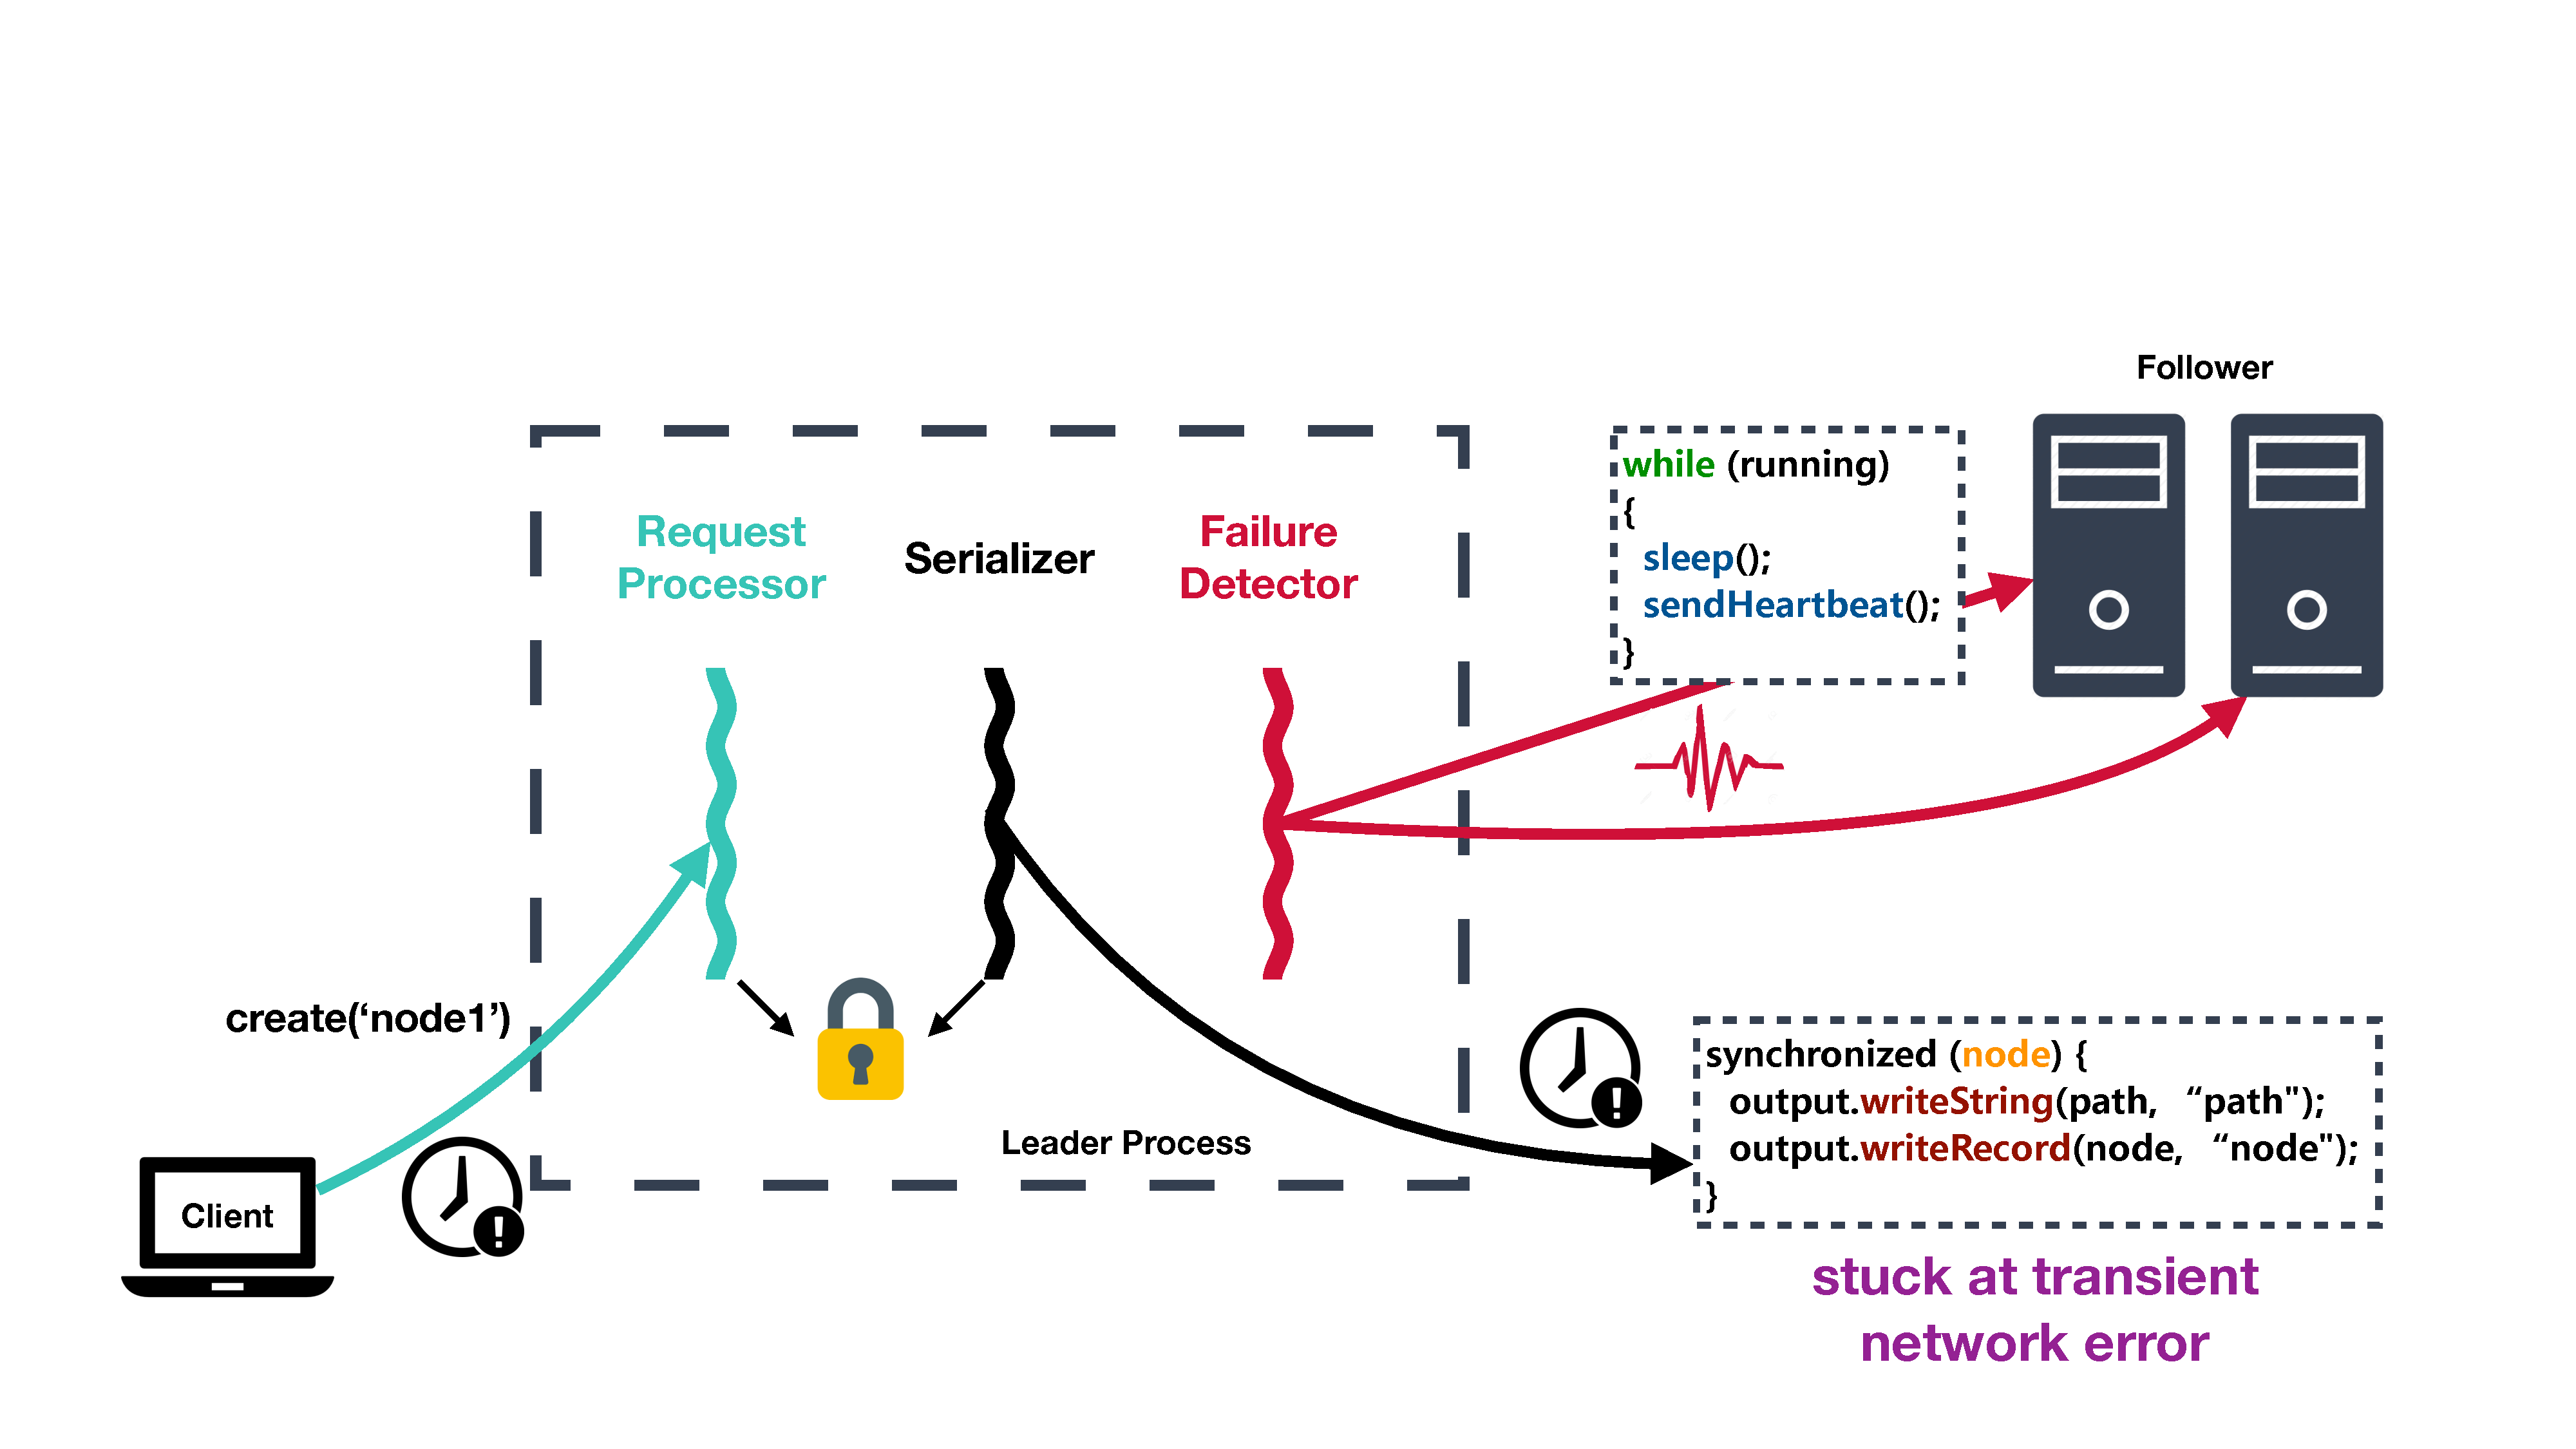
\includegraphics[width=\textwidth]{fig/example1.pdf}
    \end{center}
\end{frame}

\begin{frame}
    \frametitle{What is a Partial Failure?}
    \begin{definition}
        A partial failure is, in a process $\pi$ to be when a fault \textbf{does not} crash $\pi$ but causes safety or liveness violation or severe slowness for some functionality $R_f \subsetneq  R$

    \end{definition}
    \textbf{Scope:} In this paper, we will specify the partial failure at the \red{process} granularity instead of \blue{service}.
    \begin{center}
        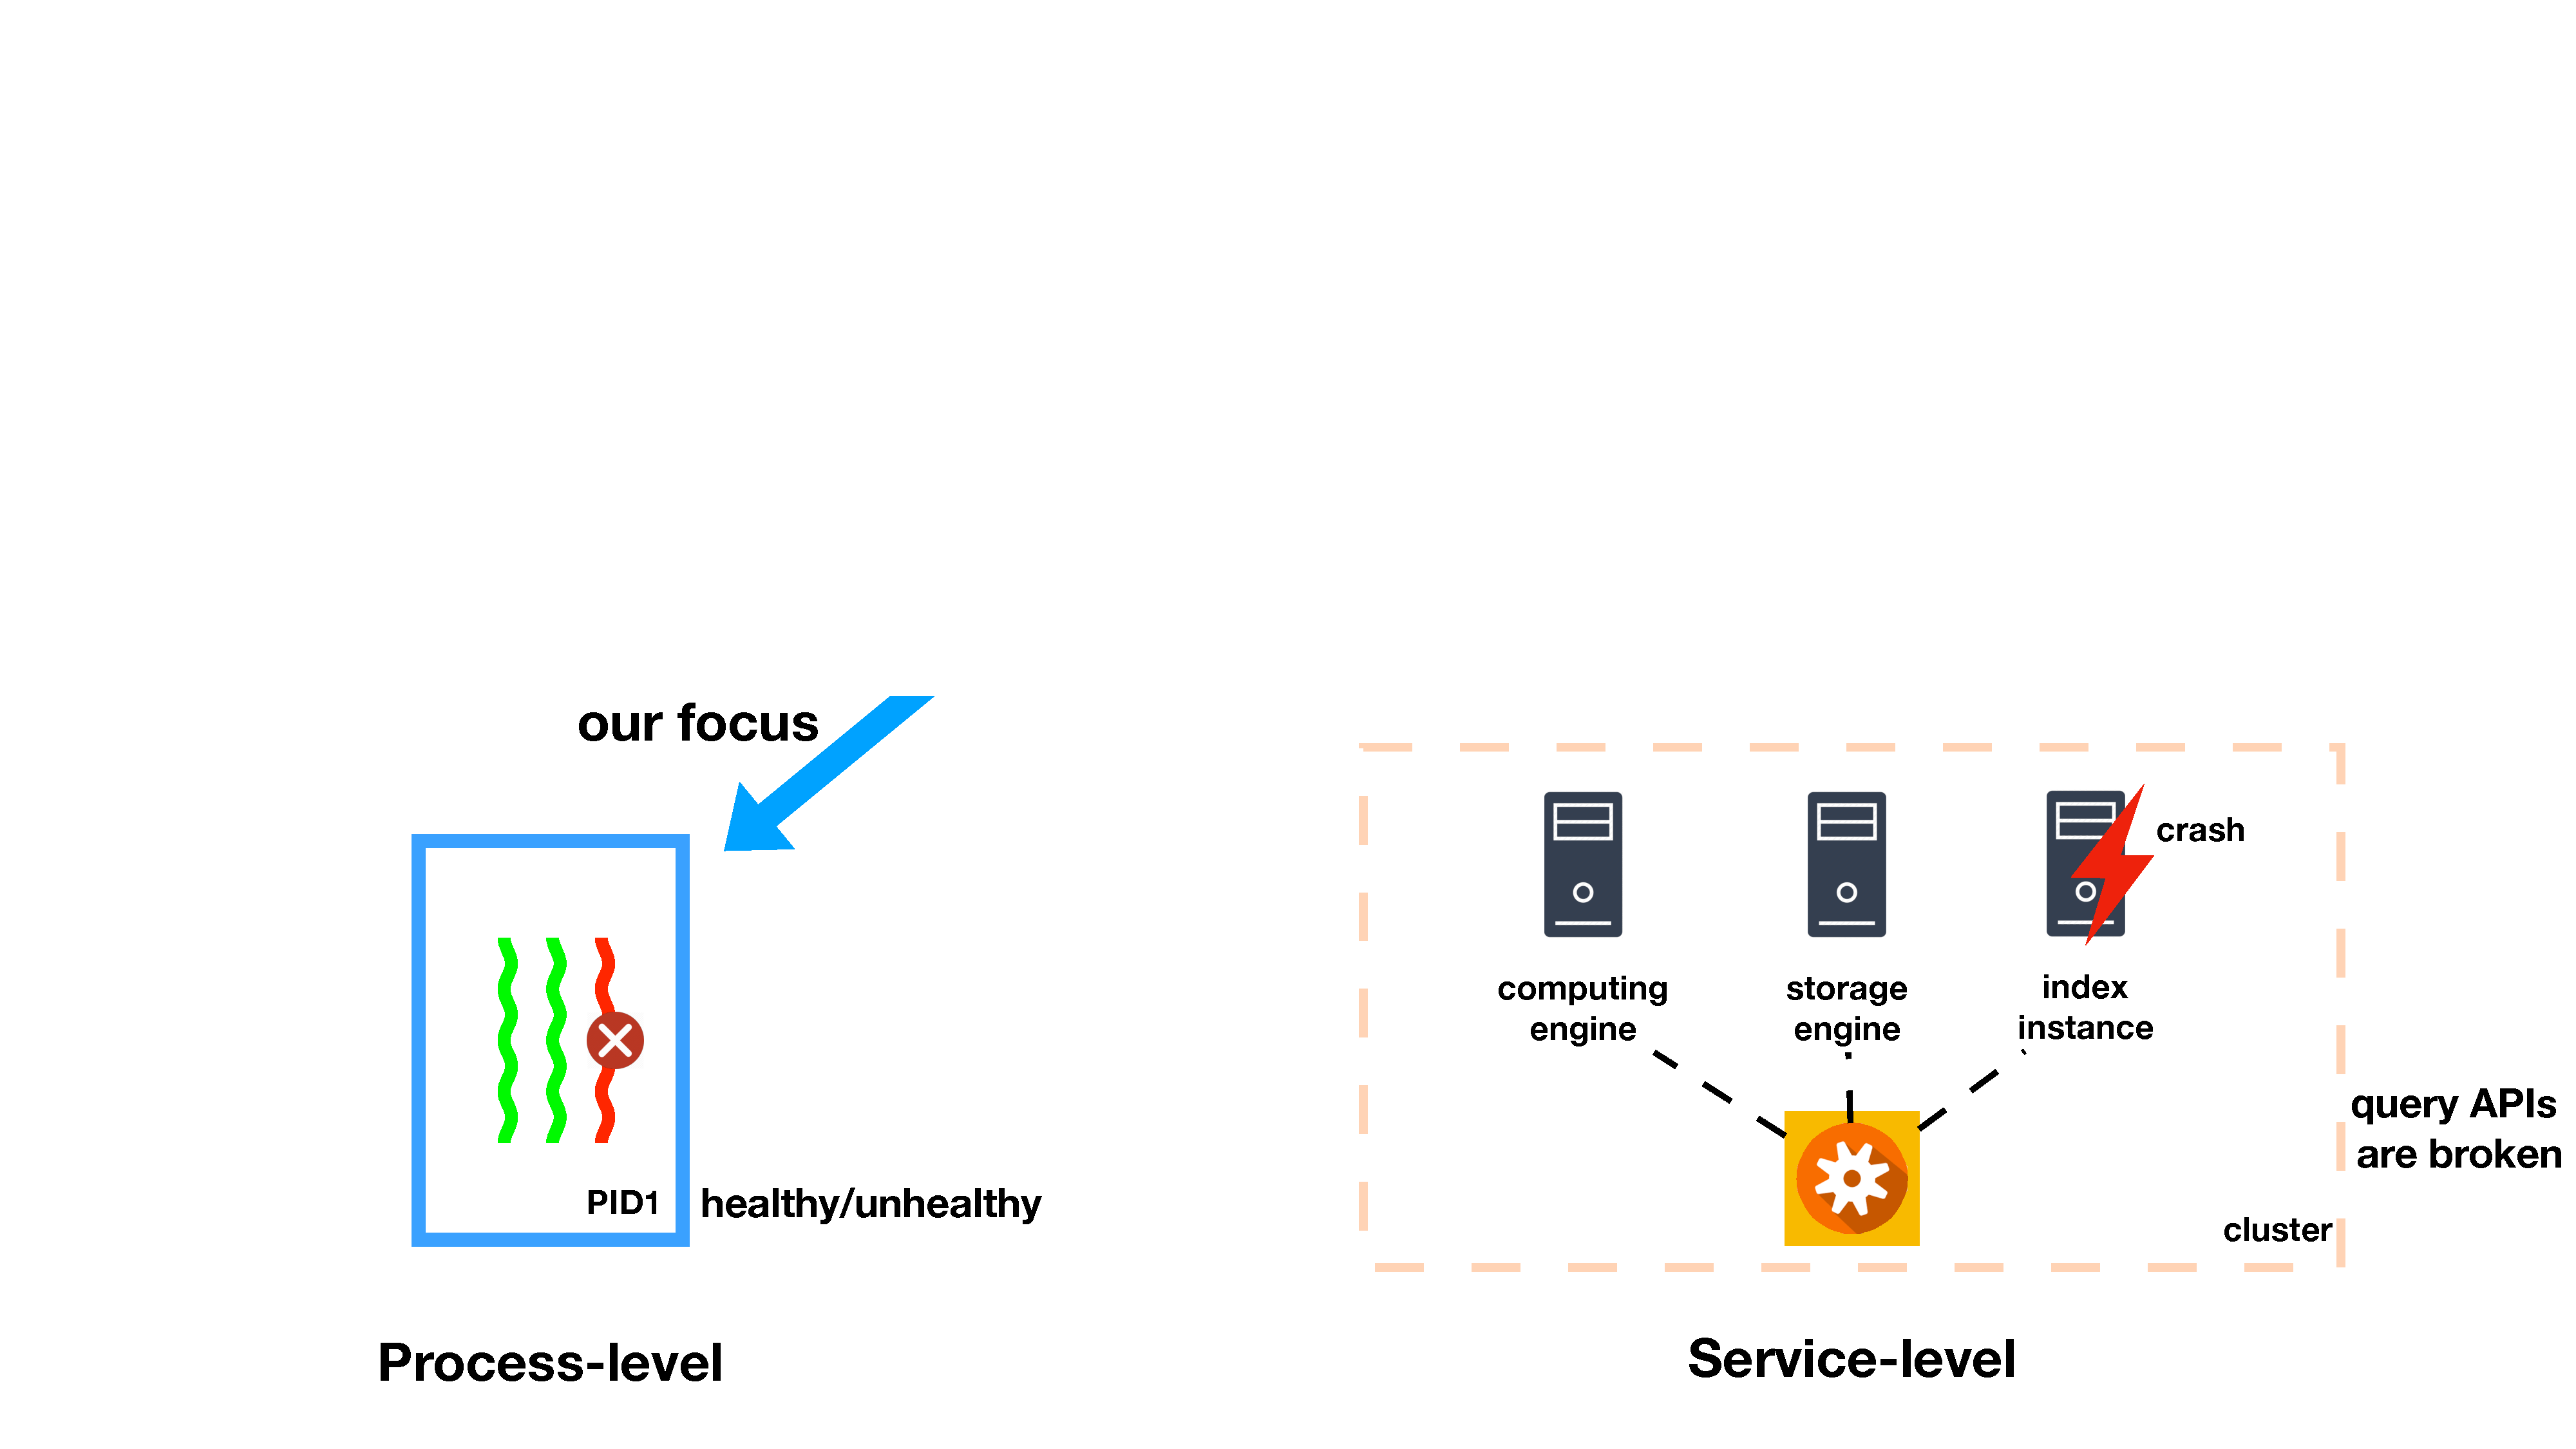
\includegraphics[width=.9\textwidth]{fig/level}
    \end{center}
\end{frame}

\section{Case Study}
\begin{frame}
    \frametitle{Study methodology}
    \begin{block}{\textbf{100 partial failure cases from five large, widely-used software systems}}
        \begin{itemize}
            \item Crawl all bug tickets tagged with critical priorities in the official
                  bug trackers
            \item Filter tickets from testing and randomly
                  sample the remaining failures tickets.
        \end{itemize}
    \end{block}

    Interestingly, \red{54\%} of them occur in the most recent \red{three} years’ software
    releases \textit{(average lifespan of all systems is \red{9} years)}
    \begin{center}
        \begin{tabular}{c|c|c|c|c}
            \toprule
            Software  & Language & Cases & Versions           & Date Range            \\
            \midrule
            ZooKeeper & Java     & 20    & 17 (3.2.1–3.5.3)   & 12/01/2009–08/28/2018 \\
            Cassandra & Java     & 20    & 19 (0.7.4–3.0.13)  & 04/22/2011–08/31/2017 \\
            HDFS      & Java     & 20    & 14 (0.20.1–3.1.0)  & 10/29/2009–08/06/2018 \\
            Apache    & C        & 20    & 16 (2.0.40–2.4.29) & 08/02/2002–03/20/2018 \\
            Mesos     & C++      & 20    & 11 (0.11.0–1.7.0)  & 04/08/2013–12/28/2018 \\
            \bottomrule
        \end{tabular}
    \end{center}
\end{frame}

\subsection{Findings}

\begin{frame}
    \frametitle{Finding 1: Root Causes are \red{Diverse}}
    \framesubtitle{Root cause distribution}
    \begin{block}{\textbf{\red{No} single uniformed or dominating root cause}\footnote{UE: uncaught error; IB: indefinite blocking; EH: buggy error handling;
                DD: deadlock; PB: performance bug; LE: logic error; IL: infinite loop; RL: resource leak.}}
        Top three (total \red{48\%}) root cause types are \blue{uncaught errors},\blue{indefinite blocking}, and \blue{buggy error handling}
    \end{block}

    \begin{center}
        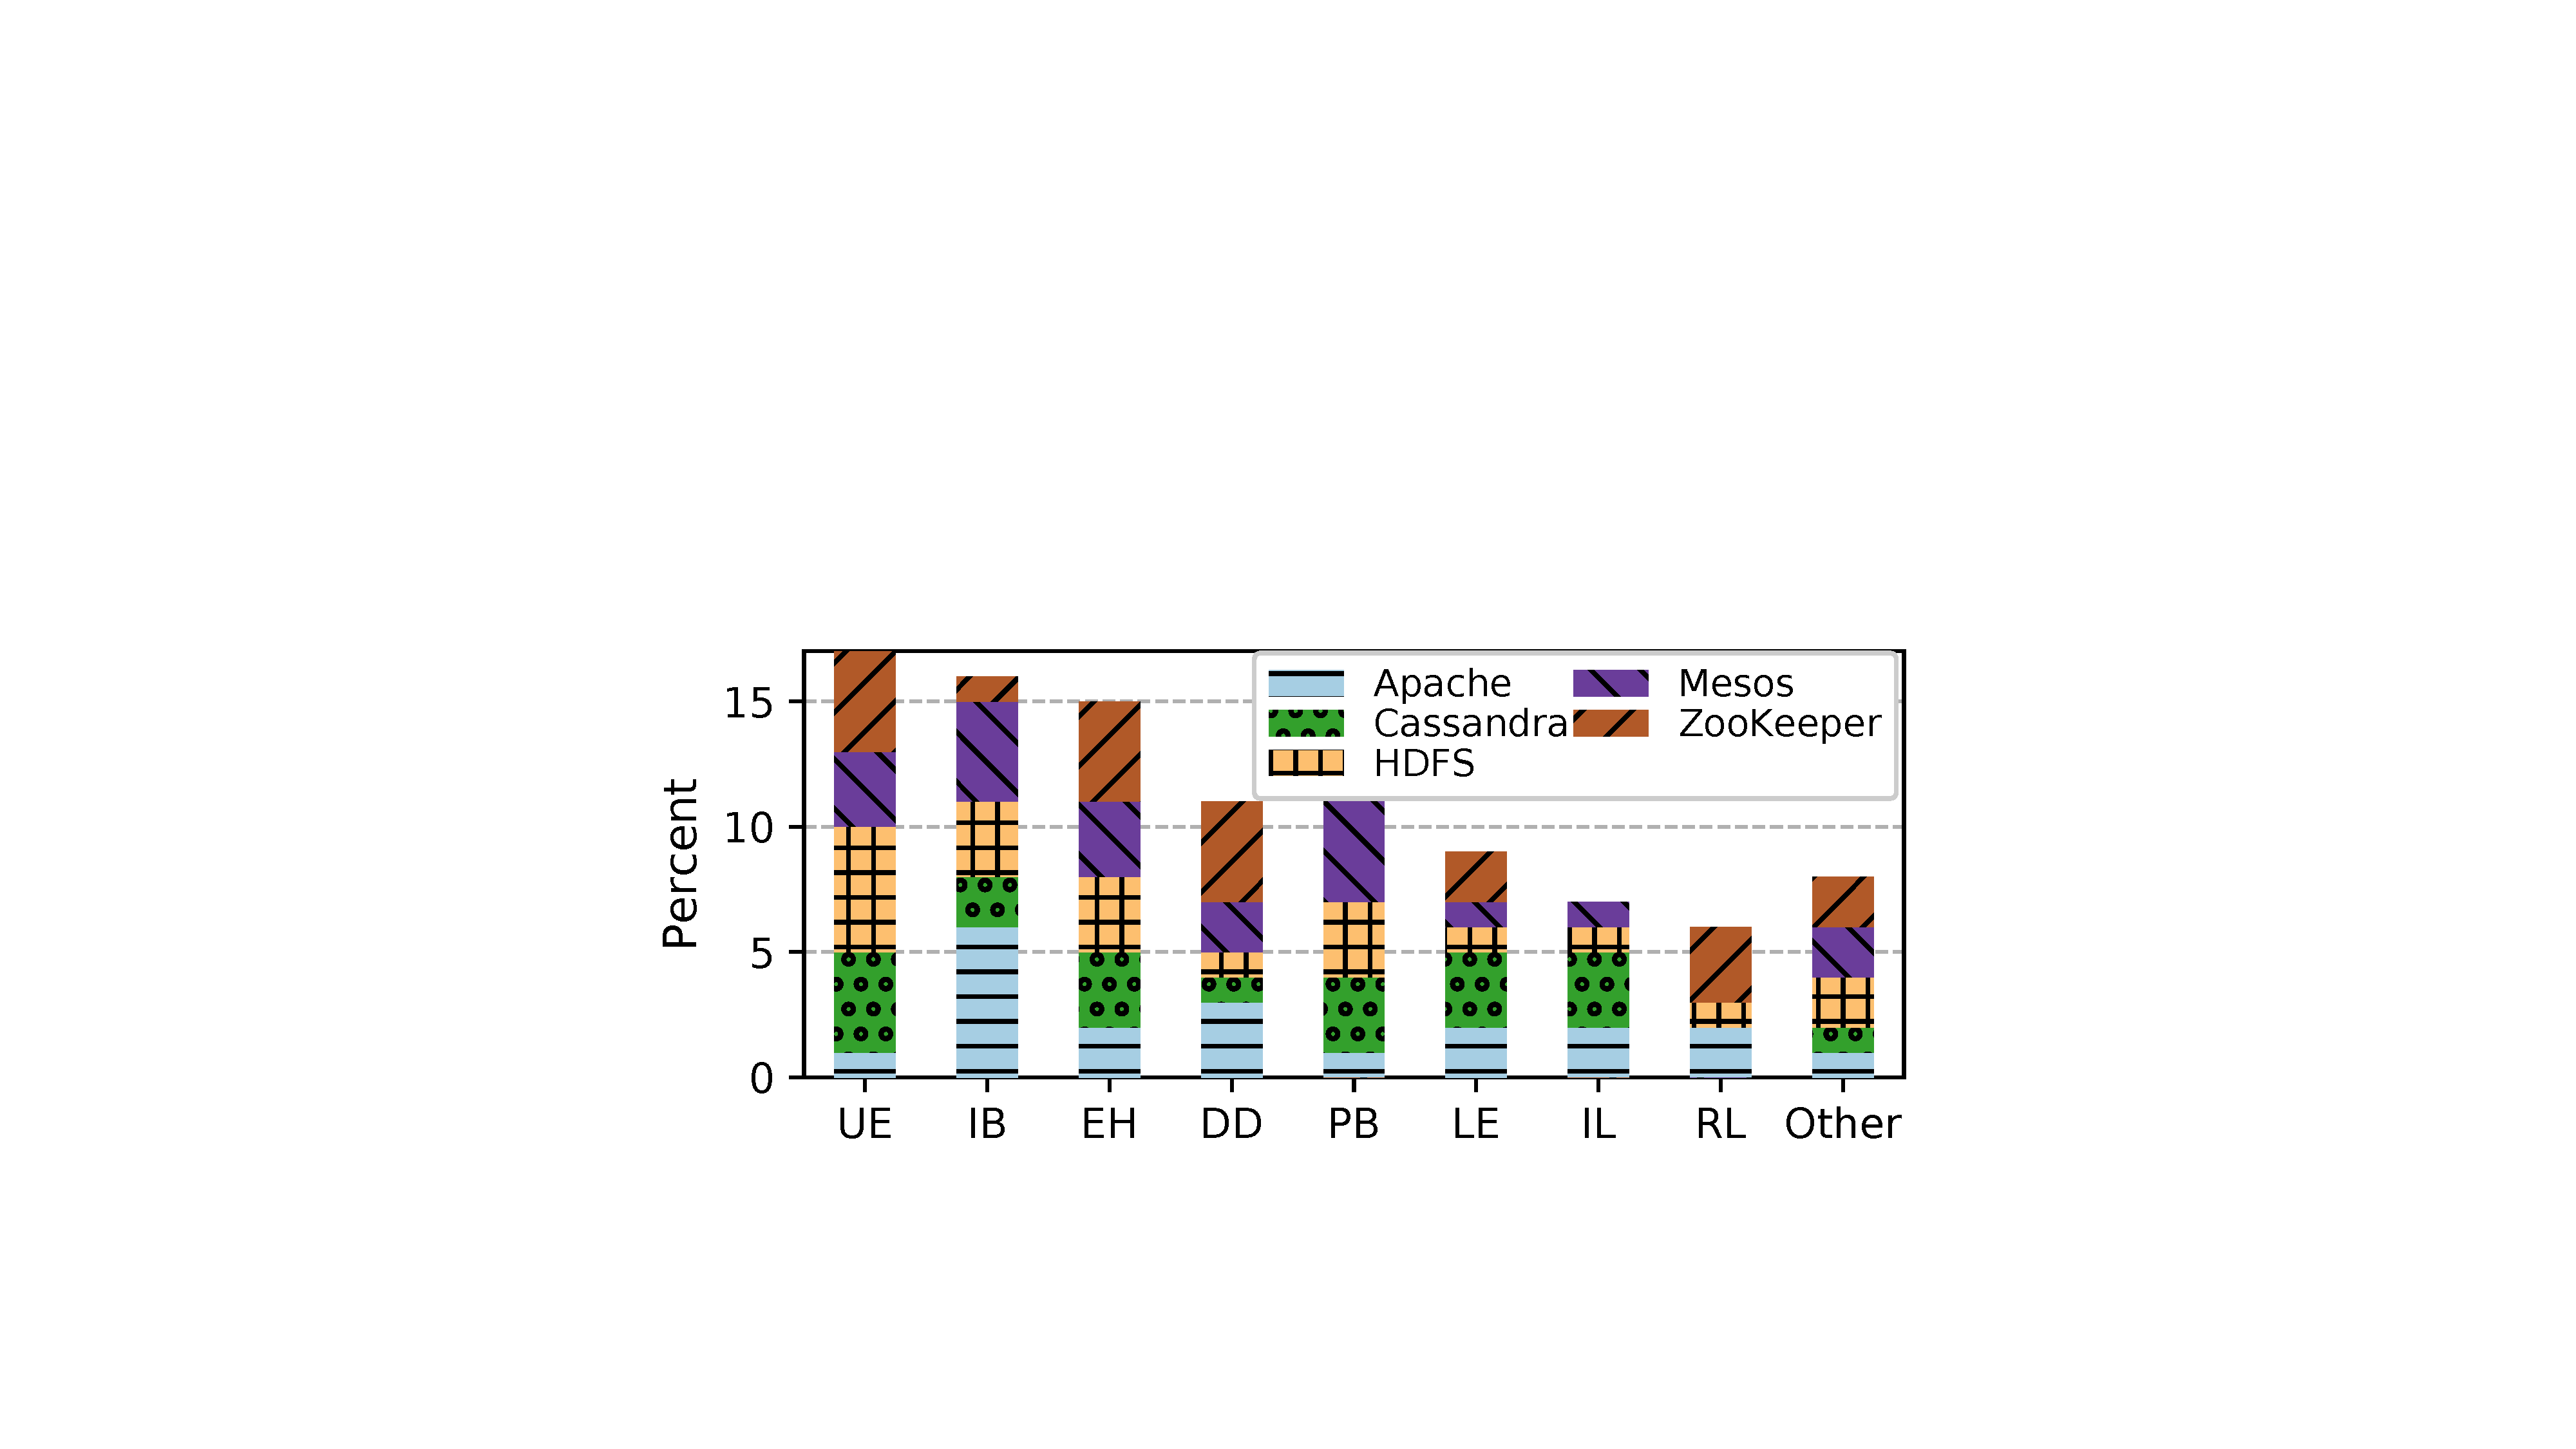
\includegraphics[width=.75\textwidth]{fig/root-cause}
    \end{center}
\end{frame}

\begin{frame}
    \frametitle{Finding 2: Nearly Half Cases Cause \red{Stuck} Issues}
    \framesubtitle{Consequence}
    Nearly half (\red{48\%}) of the partial failures cause some functionality to be \textit{\red{stuck}}.
    \begin{center}
        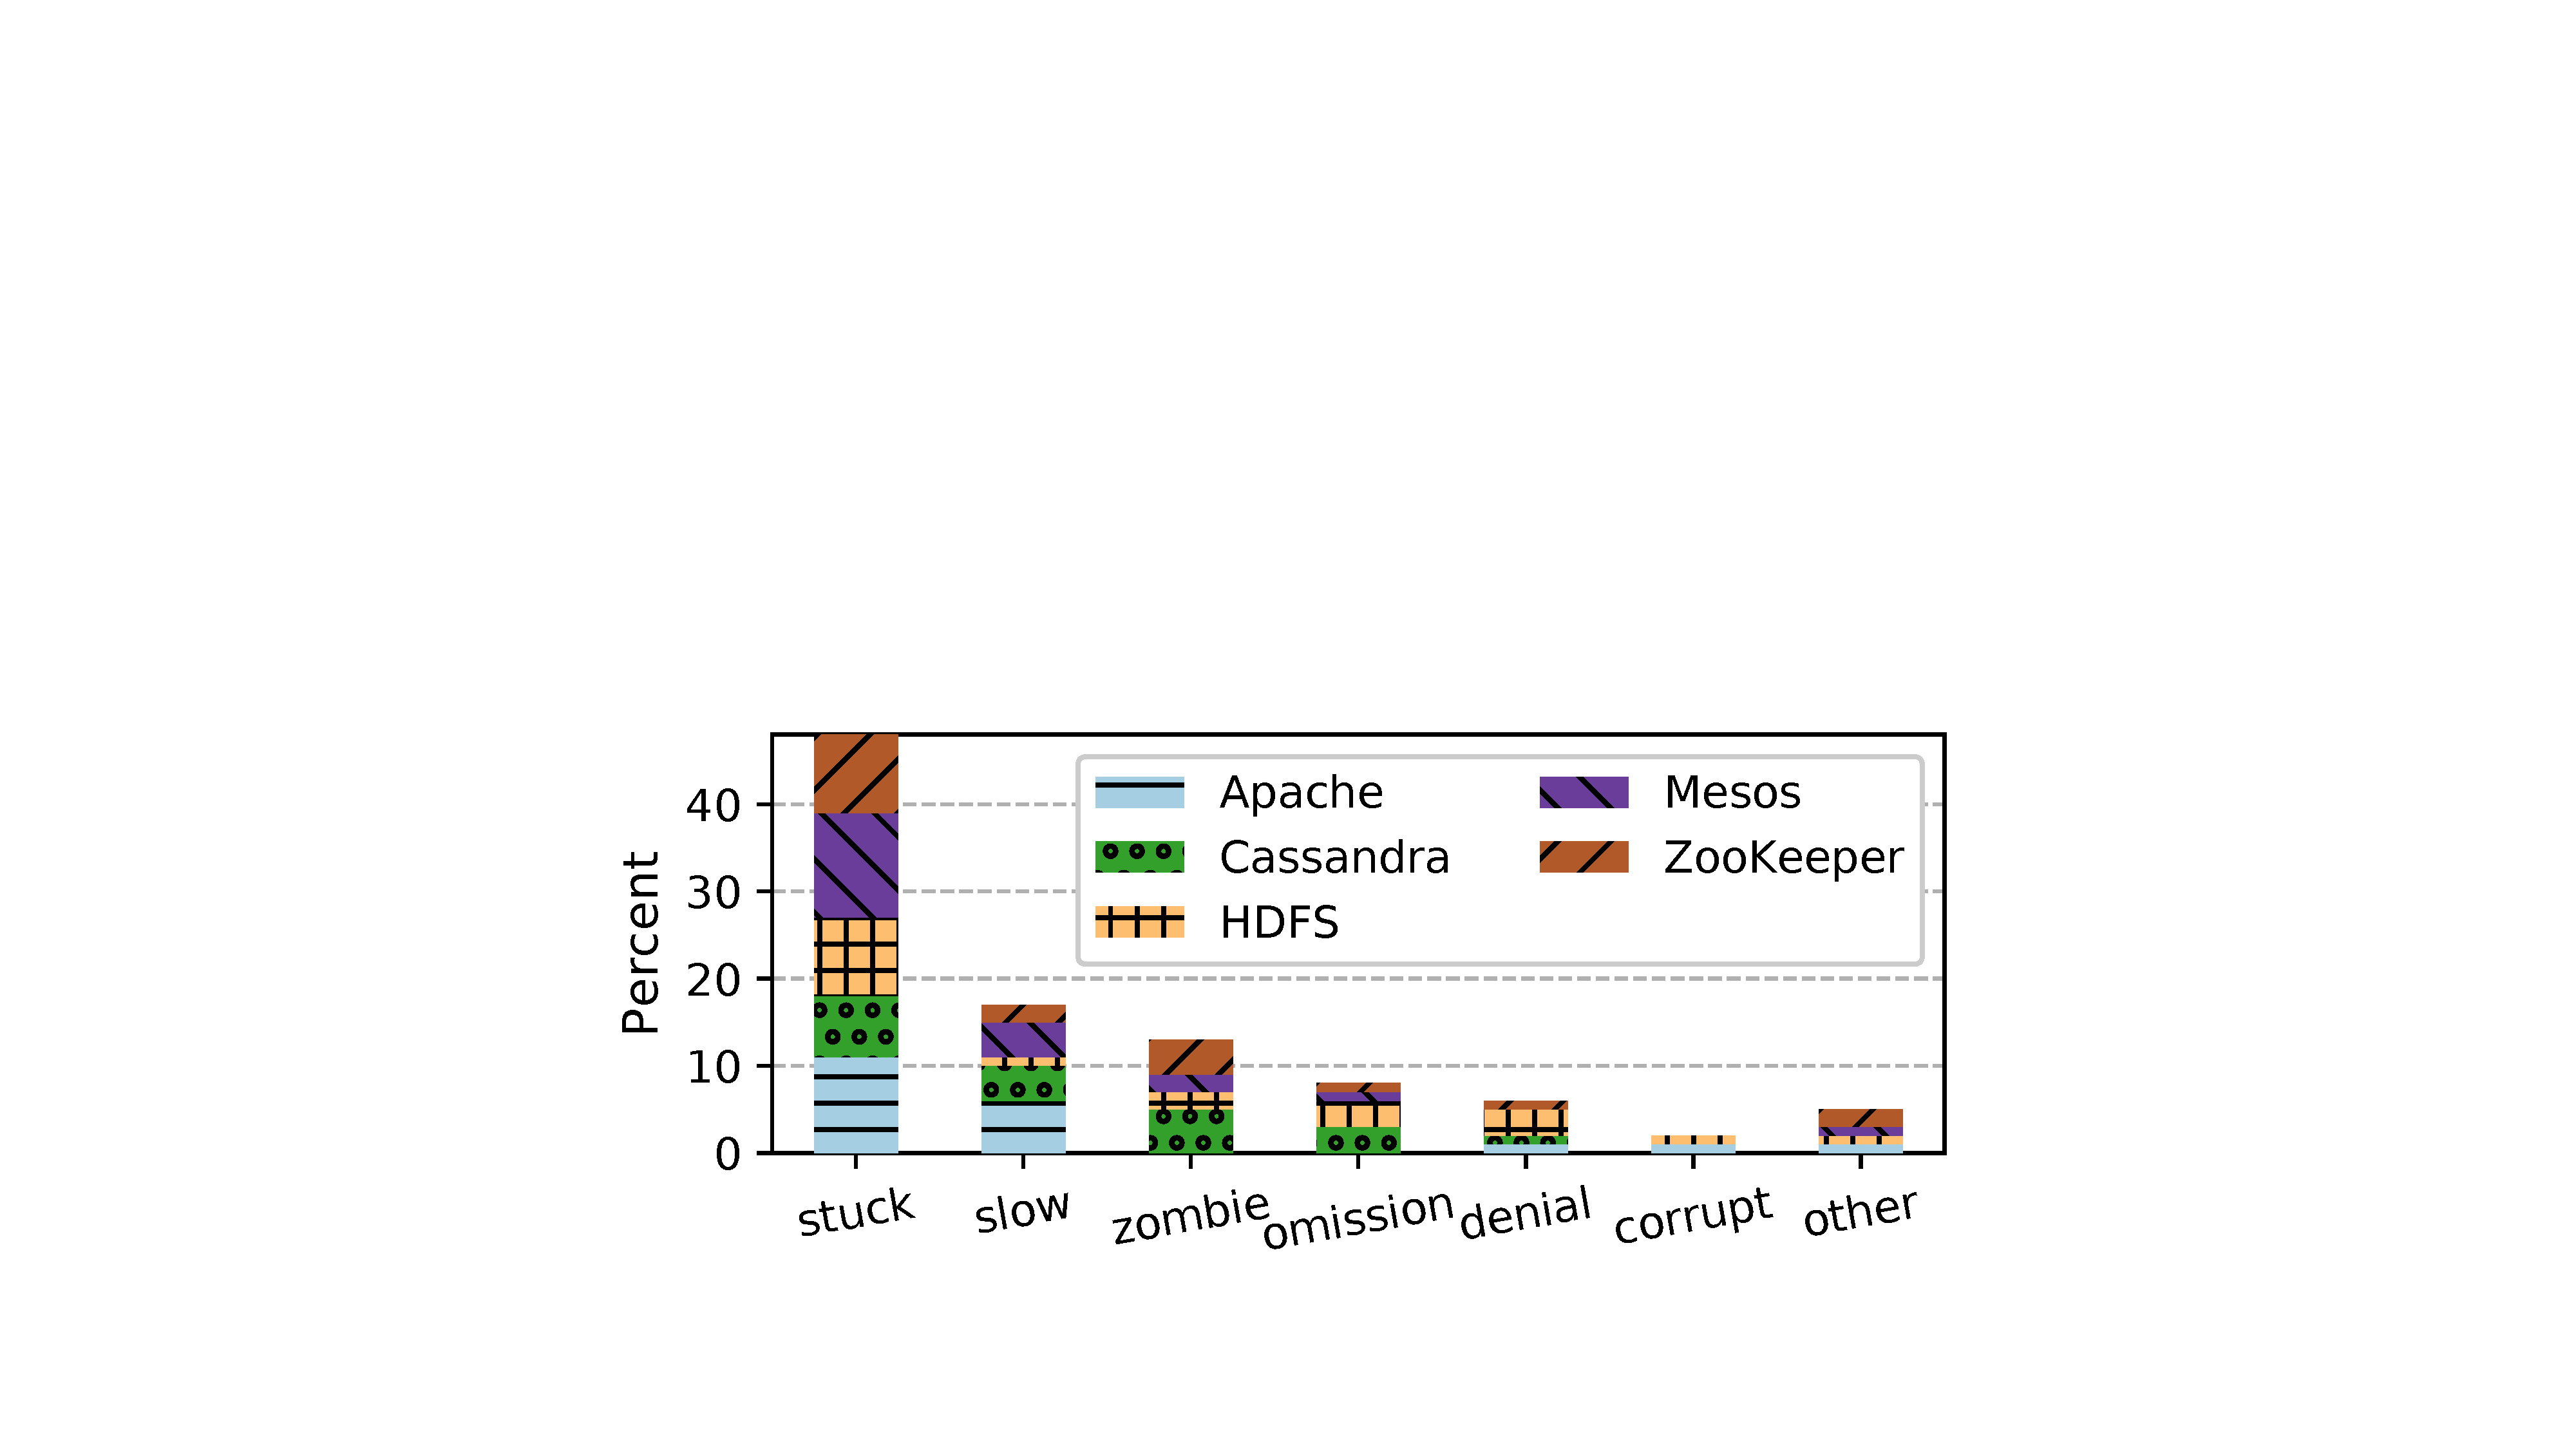
\includegraphics[width=.75\textwidth]{fig/consequence}
    \end{center}

    \red{17\%} of the partial failures cause certain operations to take a long time to complete. (i.e. \blue{\textit{slow}})
\end{frame}

\begin{frame}
    \frametitle{Other Findings: Partial Failures are Hard to Detect}
    \begin{block}{\textbf{\red{15\%} of the partial failures are silent}}
        Including data loss,corruption, inconsistency, and wrong results
    \end{block}

    \begin{block}{\textbf{\red{Most} cases are triggered by unique production workload or environment}}
        \red{71\%} of the partial failures are triggered by some \textbf{specific
            environment condition}, or \textbf{special input} in the \textbf{production}.
    \end{block}

    \begin{block}{\textbf{Debugging time is \red{long}}}
        The median diagnosis time is 6 days and 5 hours
    \end{block}

    \begin{block}{\textbf{The \red{majority (68\%)} of the failures are \red{“sticky”}}}
        The process will not recover from the faults by itself. The faulty process needs to be restarted or repaired to function again.
    \end{block}
\end{frame}

\section{Motivation}

\begin{frame}
    \frametitle{Motivation}
    What if we simply apply static or dynamic analysis?
    \framesubtitle{So how to detect and localize a partial failure in a big software?}
    \begin{columns}
        \begin{column}{.5\textwidth}


            \begin{block}{Static Analysis?}
                \begin{itemize}
                    \item no unique production env/workload
                    \item unable to detect run-time problem
                \end{itemize}
            \end{block}



        \end{column}

        \begin{column}{.48\textwidth}
            \begin{block}{Dynamic Analysis?}
                \begin{itemize}
                    \item existing detectors are too shallow
                    \item unable to  localize failures
                \end{itemize}
            \end{block}
        \end{column}
    \end{columns}

    \vspace{1em}

    Ask developers to manually add defensive checks?

    \begin{block}{Manual vs generated checkers}
        \textbf{Systematically} generated checkers to ease developers’ burden
        \begin{itemize}
            \item challenge: difficult to automate for all cases
            \item opportunity: most of partial failures do not rely on deep semantic understanding
                  to detect, such checkers can potentially be automatically constructed
        \end{itemize}
    \end{block}
\end{frame}

\section{Proposed Design}

\subsection{Ideas}

\begin{frame}
    \frametitle{Intersection Principle}

    Construct
    customized checkers that \textbf{intersect} with the execution of a monitored process:

    \begin{center}
        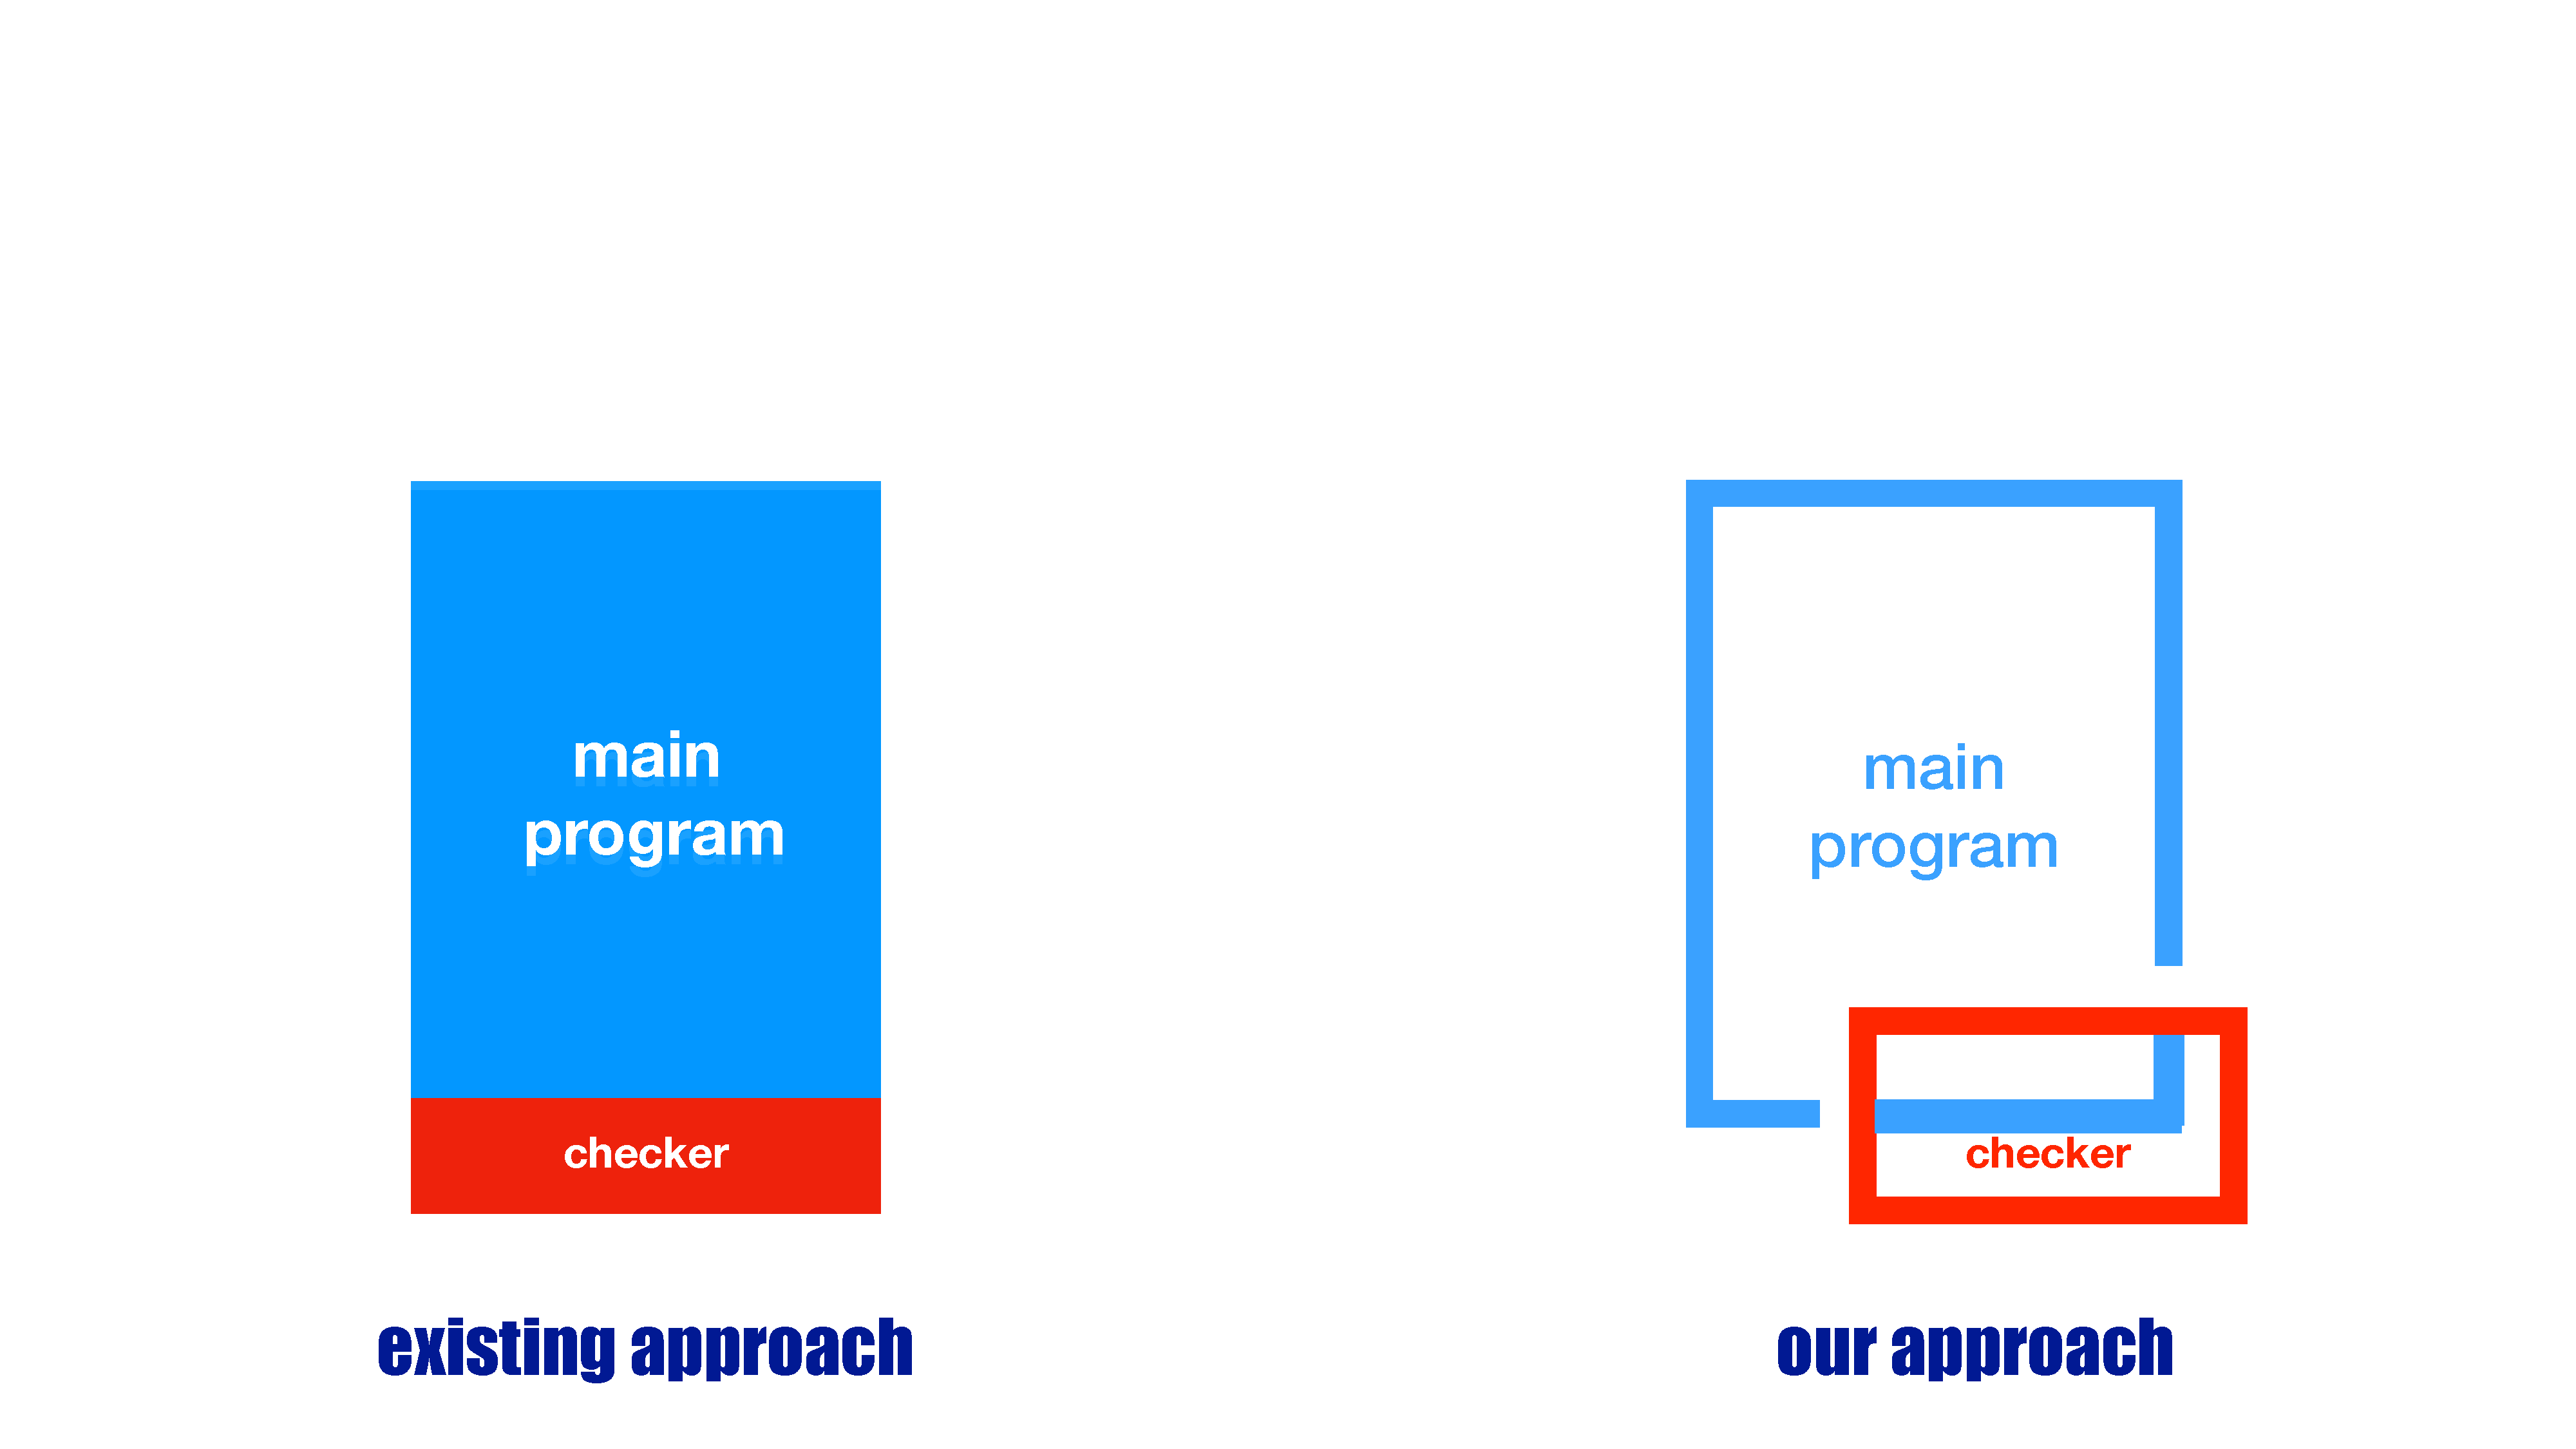
\includegraphics[width=.85\textwidth]{fig/intersect.pdf}
    \end{center}
\end{frame}

\begin{frame}
    \frametitle{Intrinsic watchdog: Runtime}
    % \framesubtitle{Follows Intersection Principle}
    An intrinsic watchdog is a dedicated monitoring extension for a process

    \begin{center}
        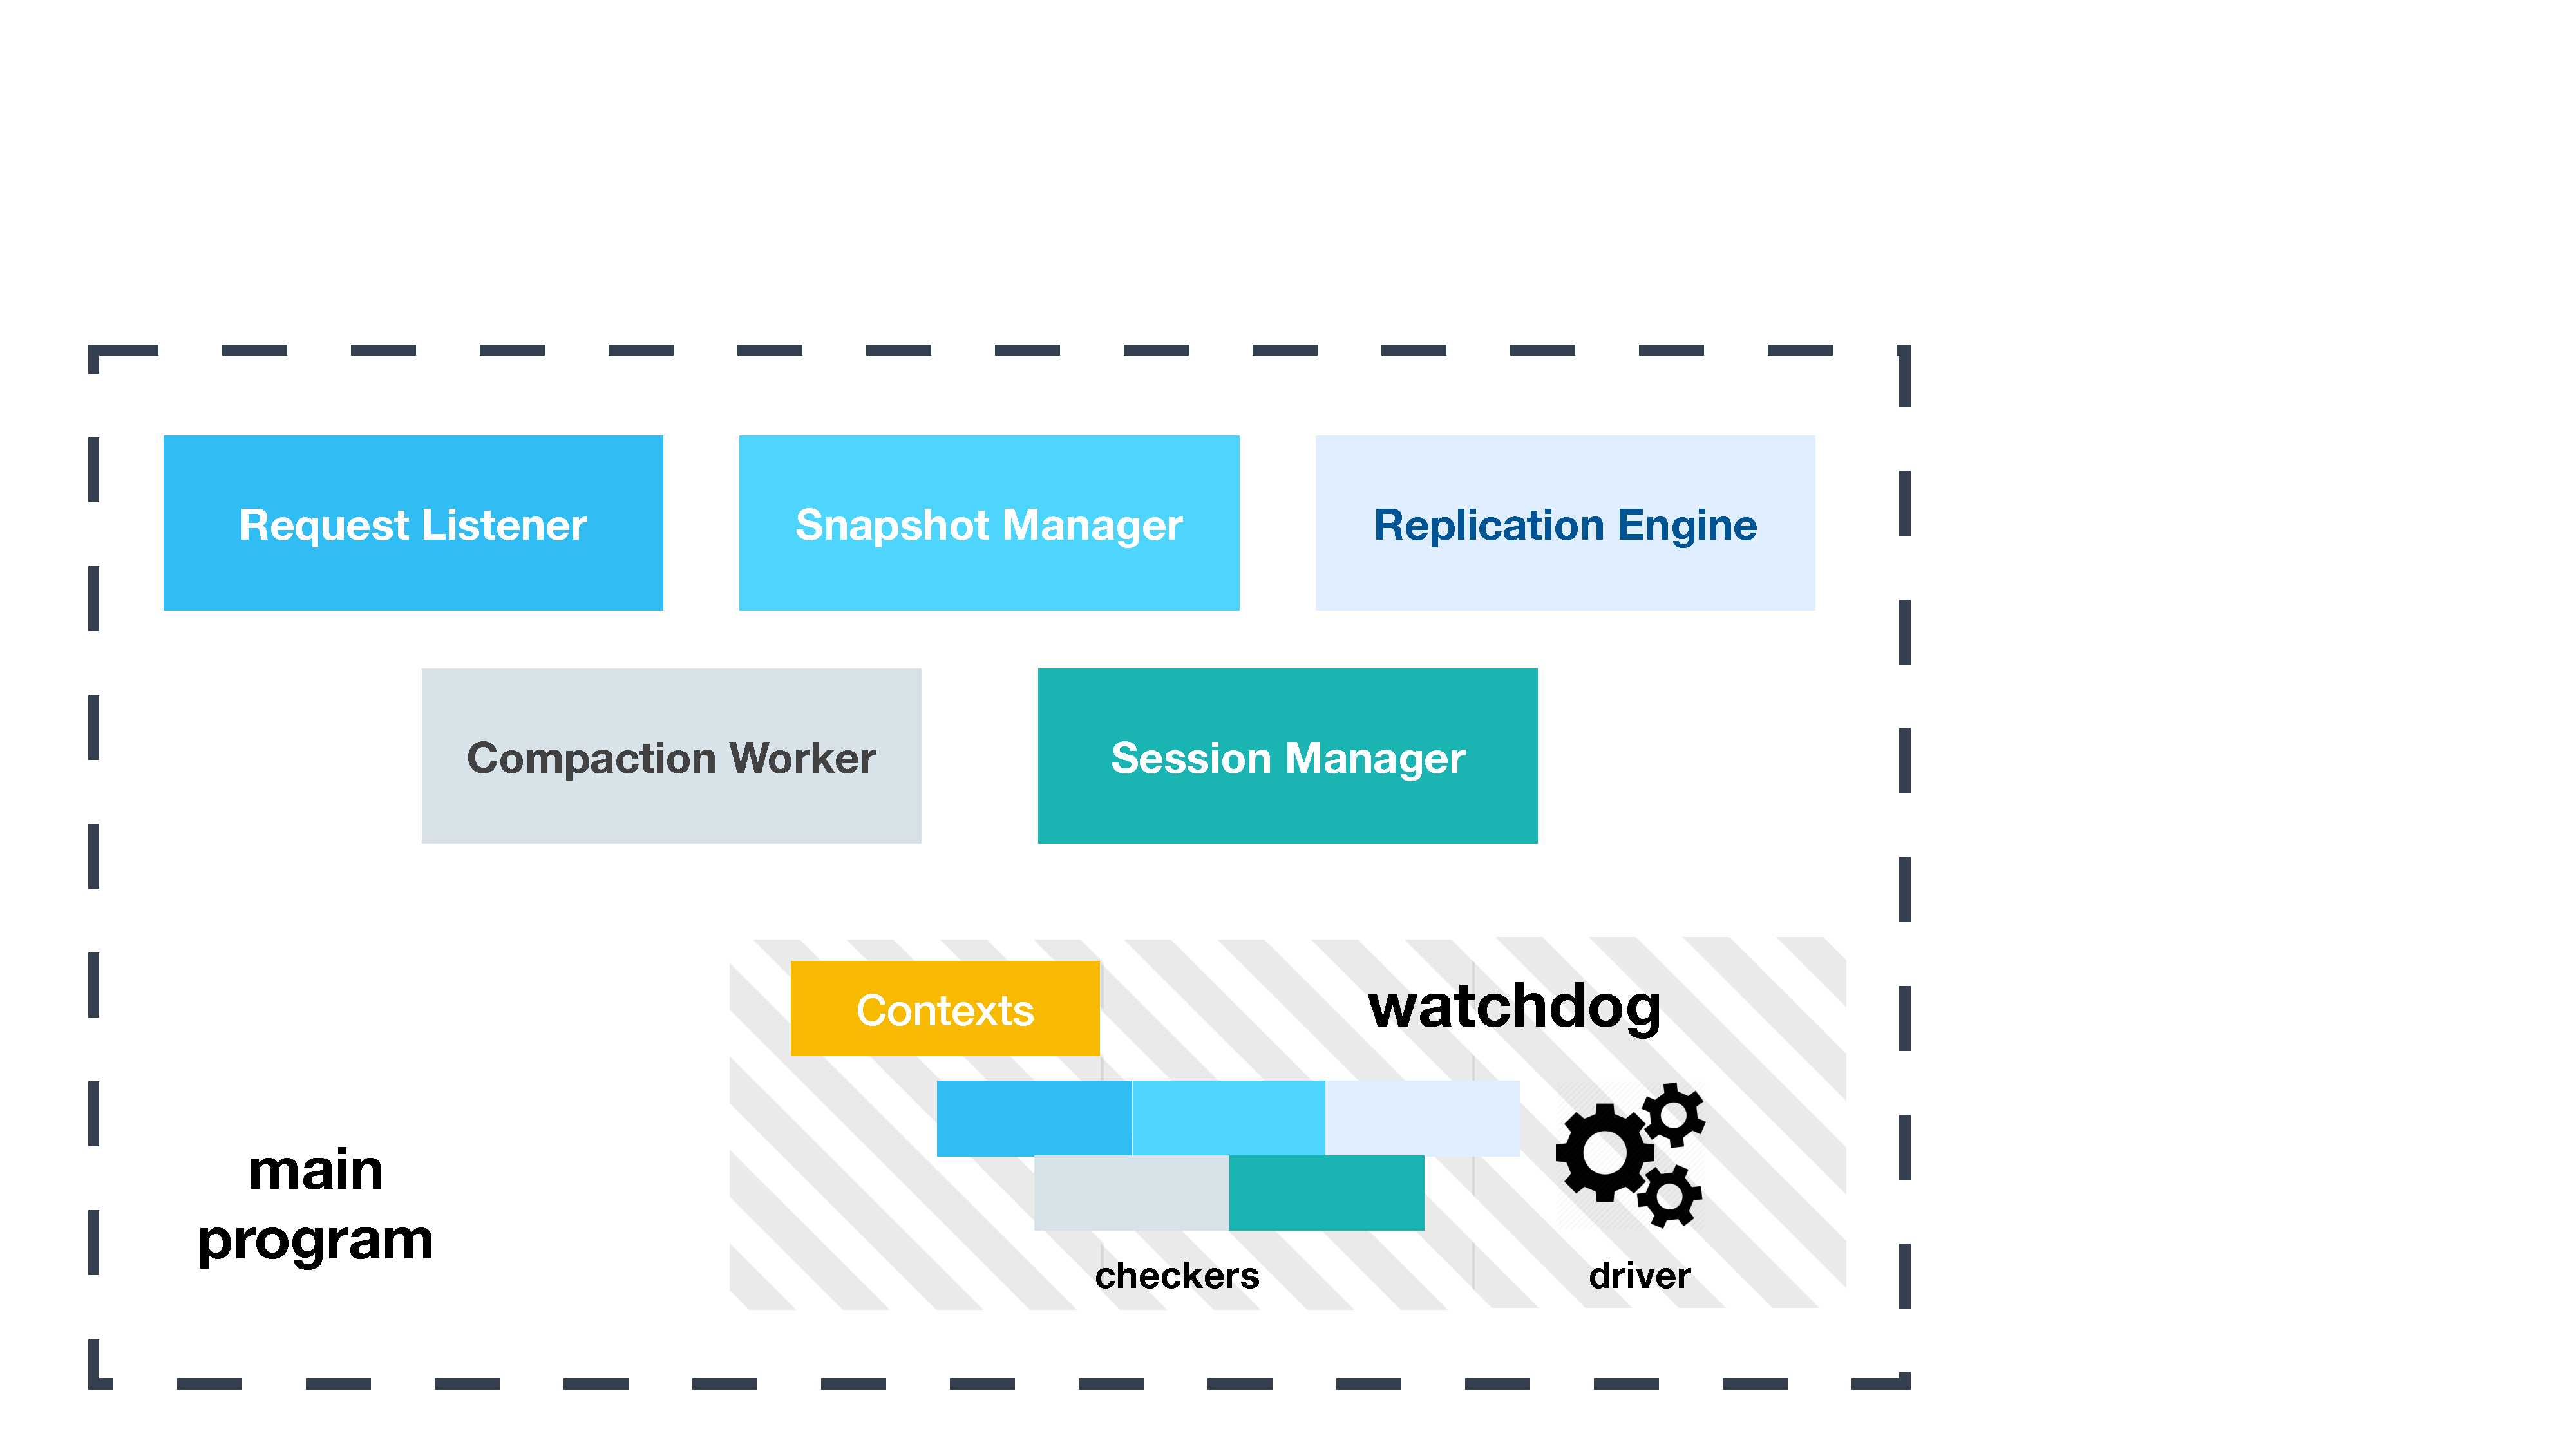
\includegraphics[width=.75\textwidth]{fig/watchdog.pdf}
    \end{center}
\end{frame}

\begin{frame}
    \frametitle{Intrinsic watchdog: How it works?}

    \begin{center}
        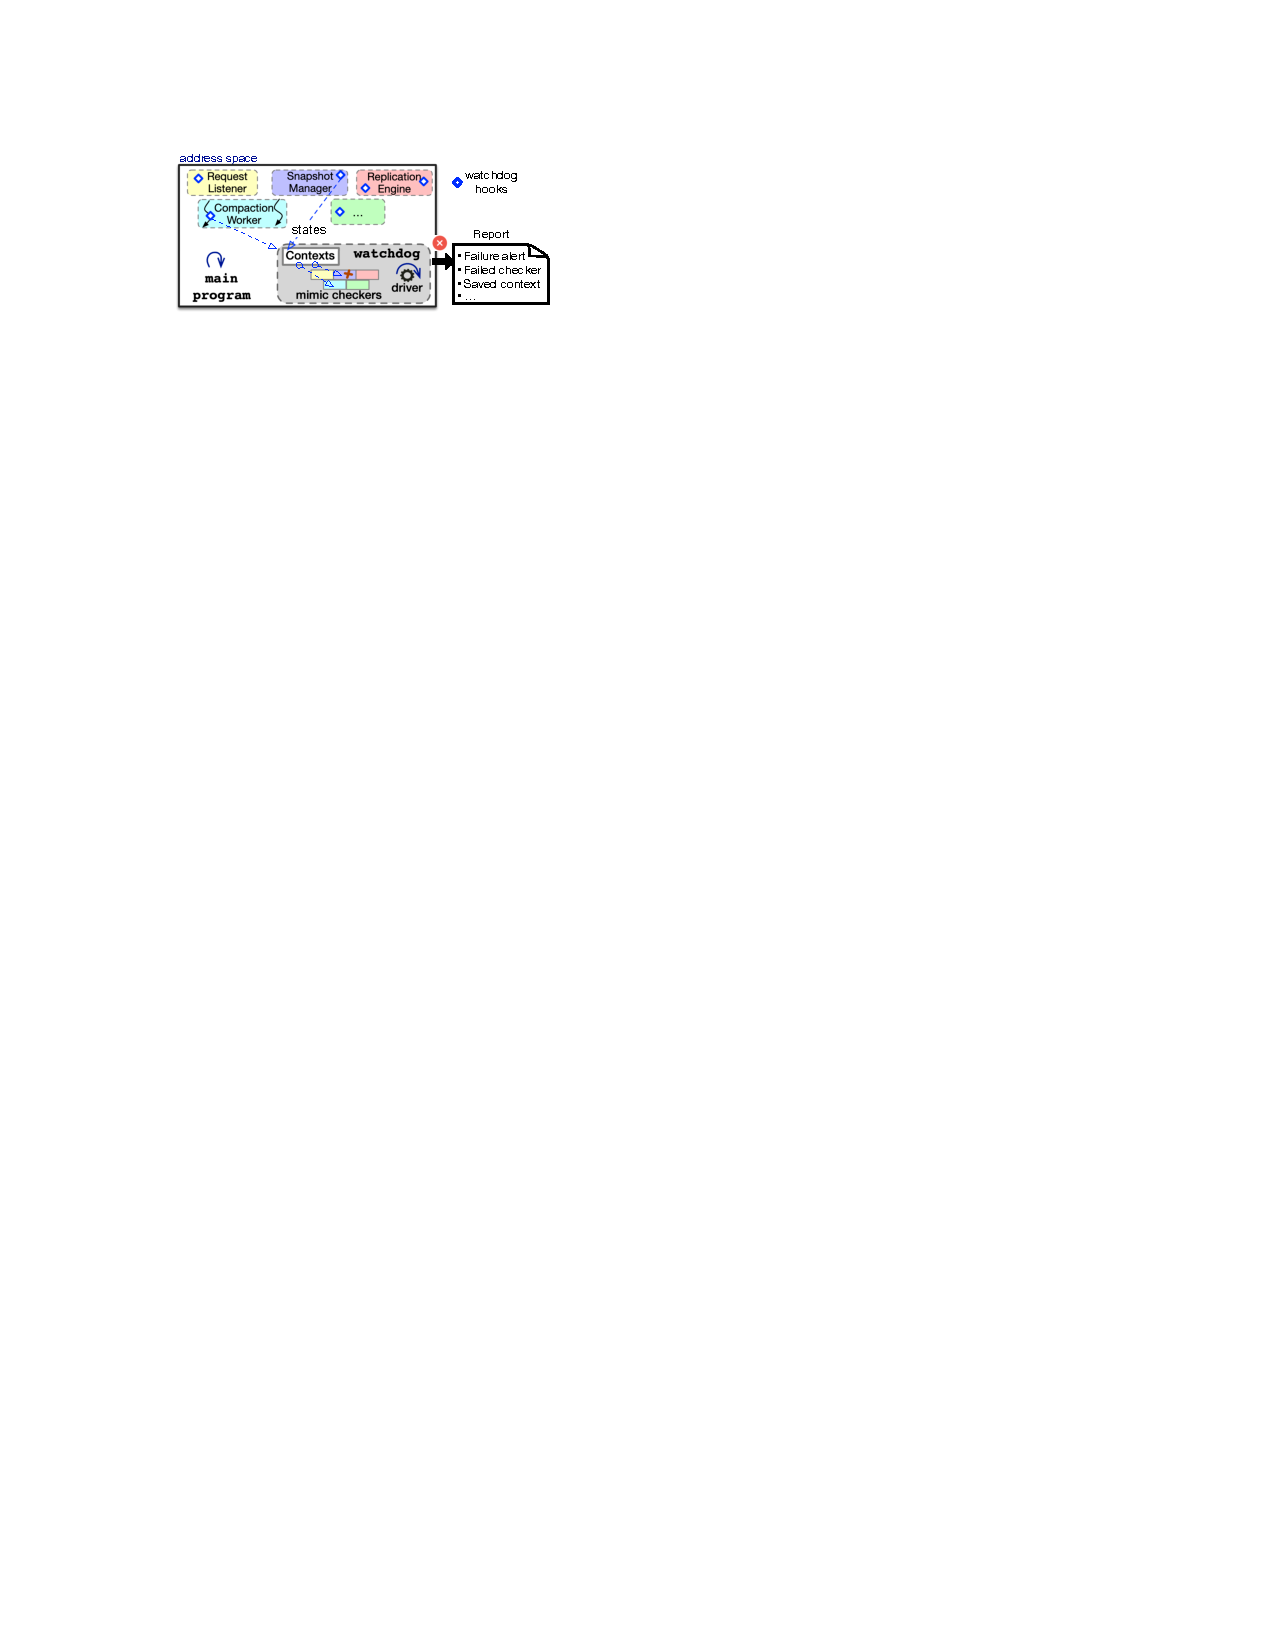
\includegraphics[width=.9\textwidth]{fig/exmaple}
    \end{center}

\end{frame}

\begin{frame}{Characteristic I: Customized}
    \begin{itemize}
        \item Regularly executes a set of checkers tailored to different modules
        \item Selects some representative operations from each
              module
    \end{itemize}

    \begin{center}
        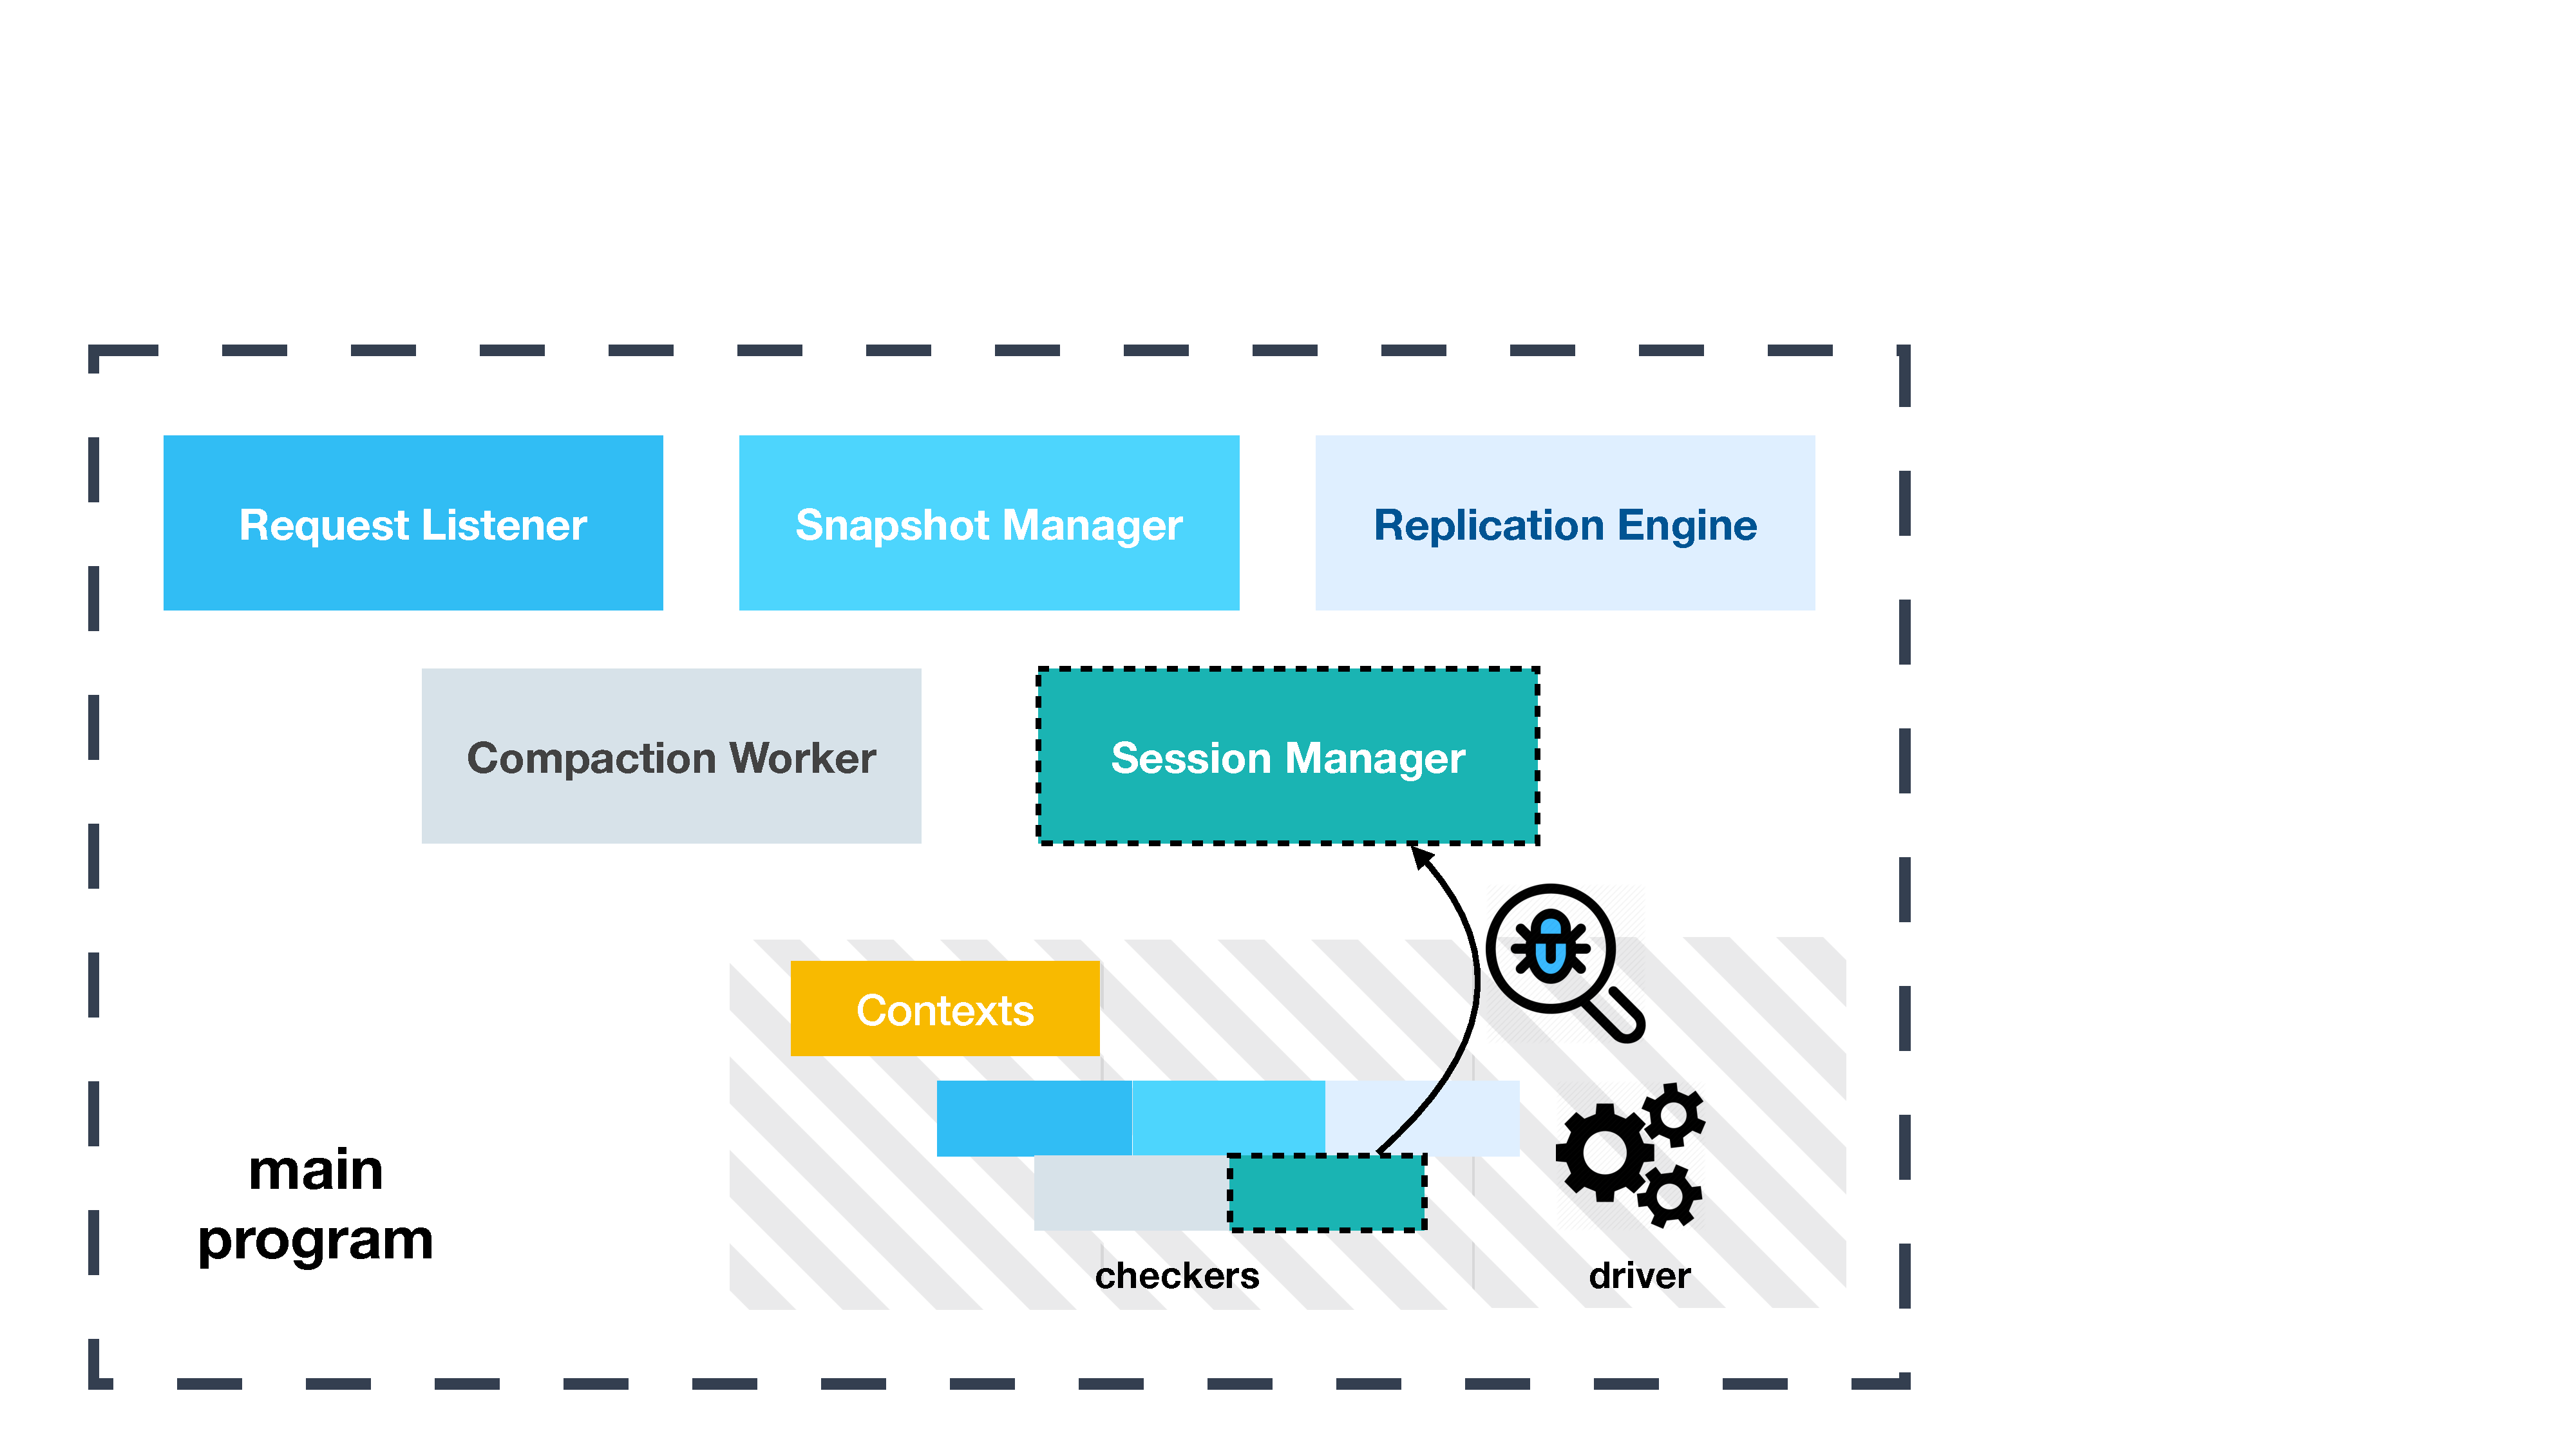
\includegraphics[width=.75\textwidth]{fig/customized}
    \end{center}
\end{frame}

\begin{frame}{Characteristic II: Stateful}
    \begin{columns}

        \begin{column}{.5\textwidth}
            To synchronized states, introduce
            \begin{block}{\textbf{Context}}
                \begin{itemize}
                    \item bound
                          to each checker
                    \item  holds all the arguments needed for the
                          checker execution
                    \item  synchronized with the program state through hooks in the main program
                    \item update with current state when hooks reached
                \end{itemize}
            \end{block}
        \end{column}

        \begin{column}{.5\textwidth}

            \begin{center}
                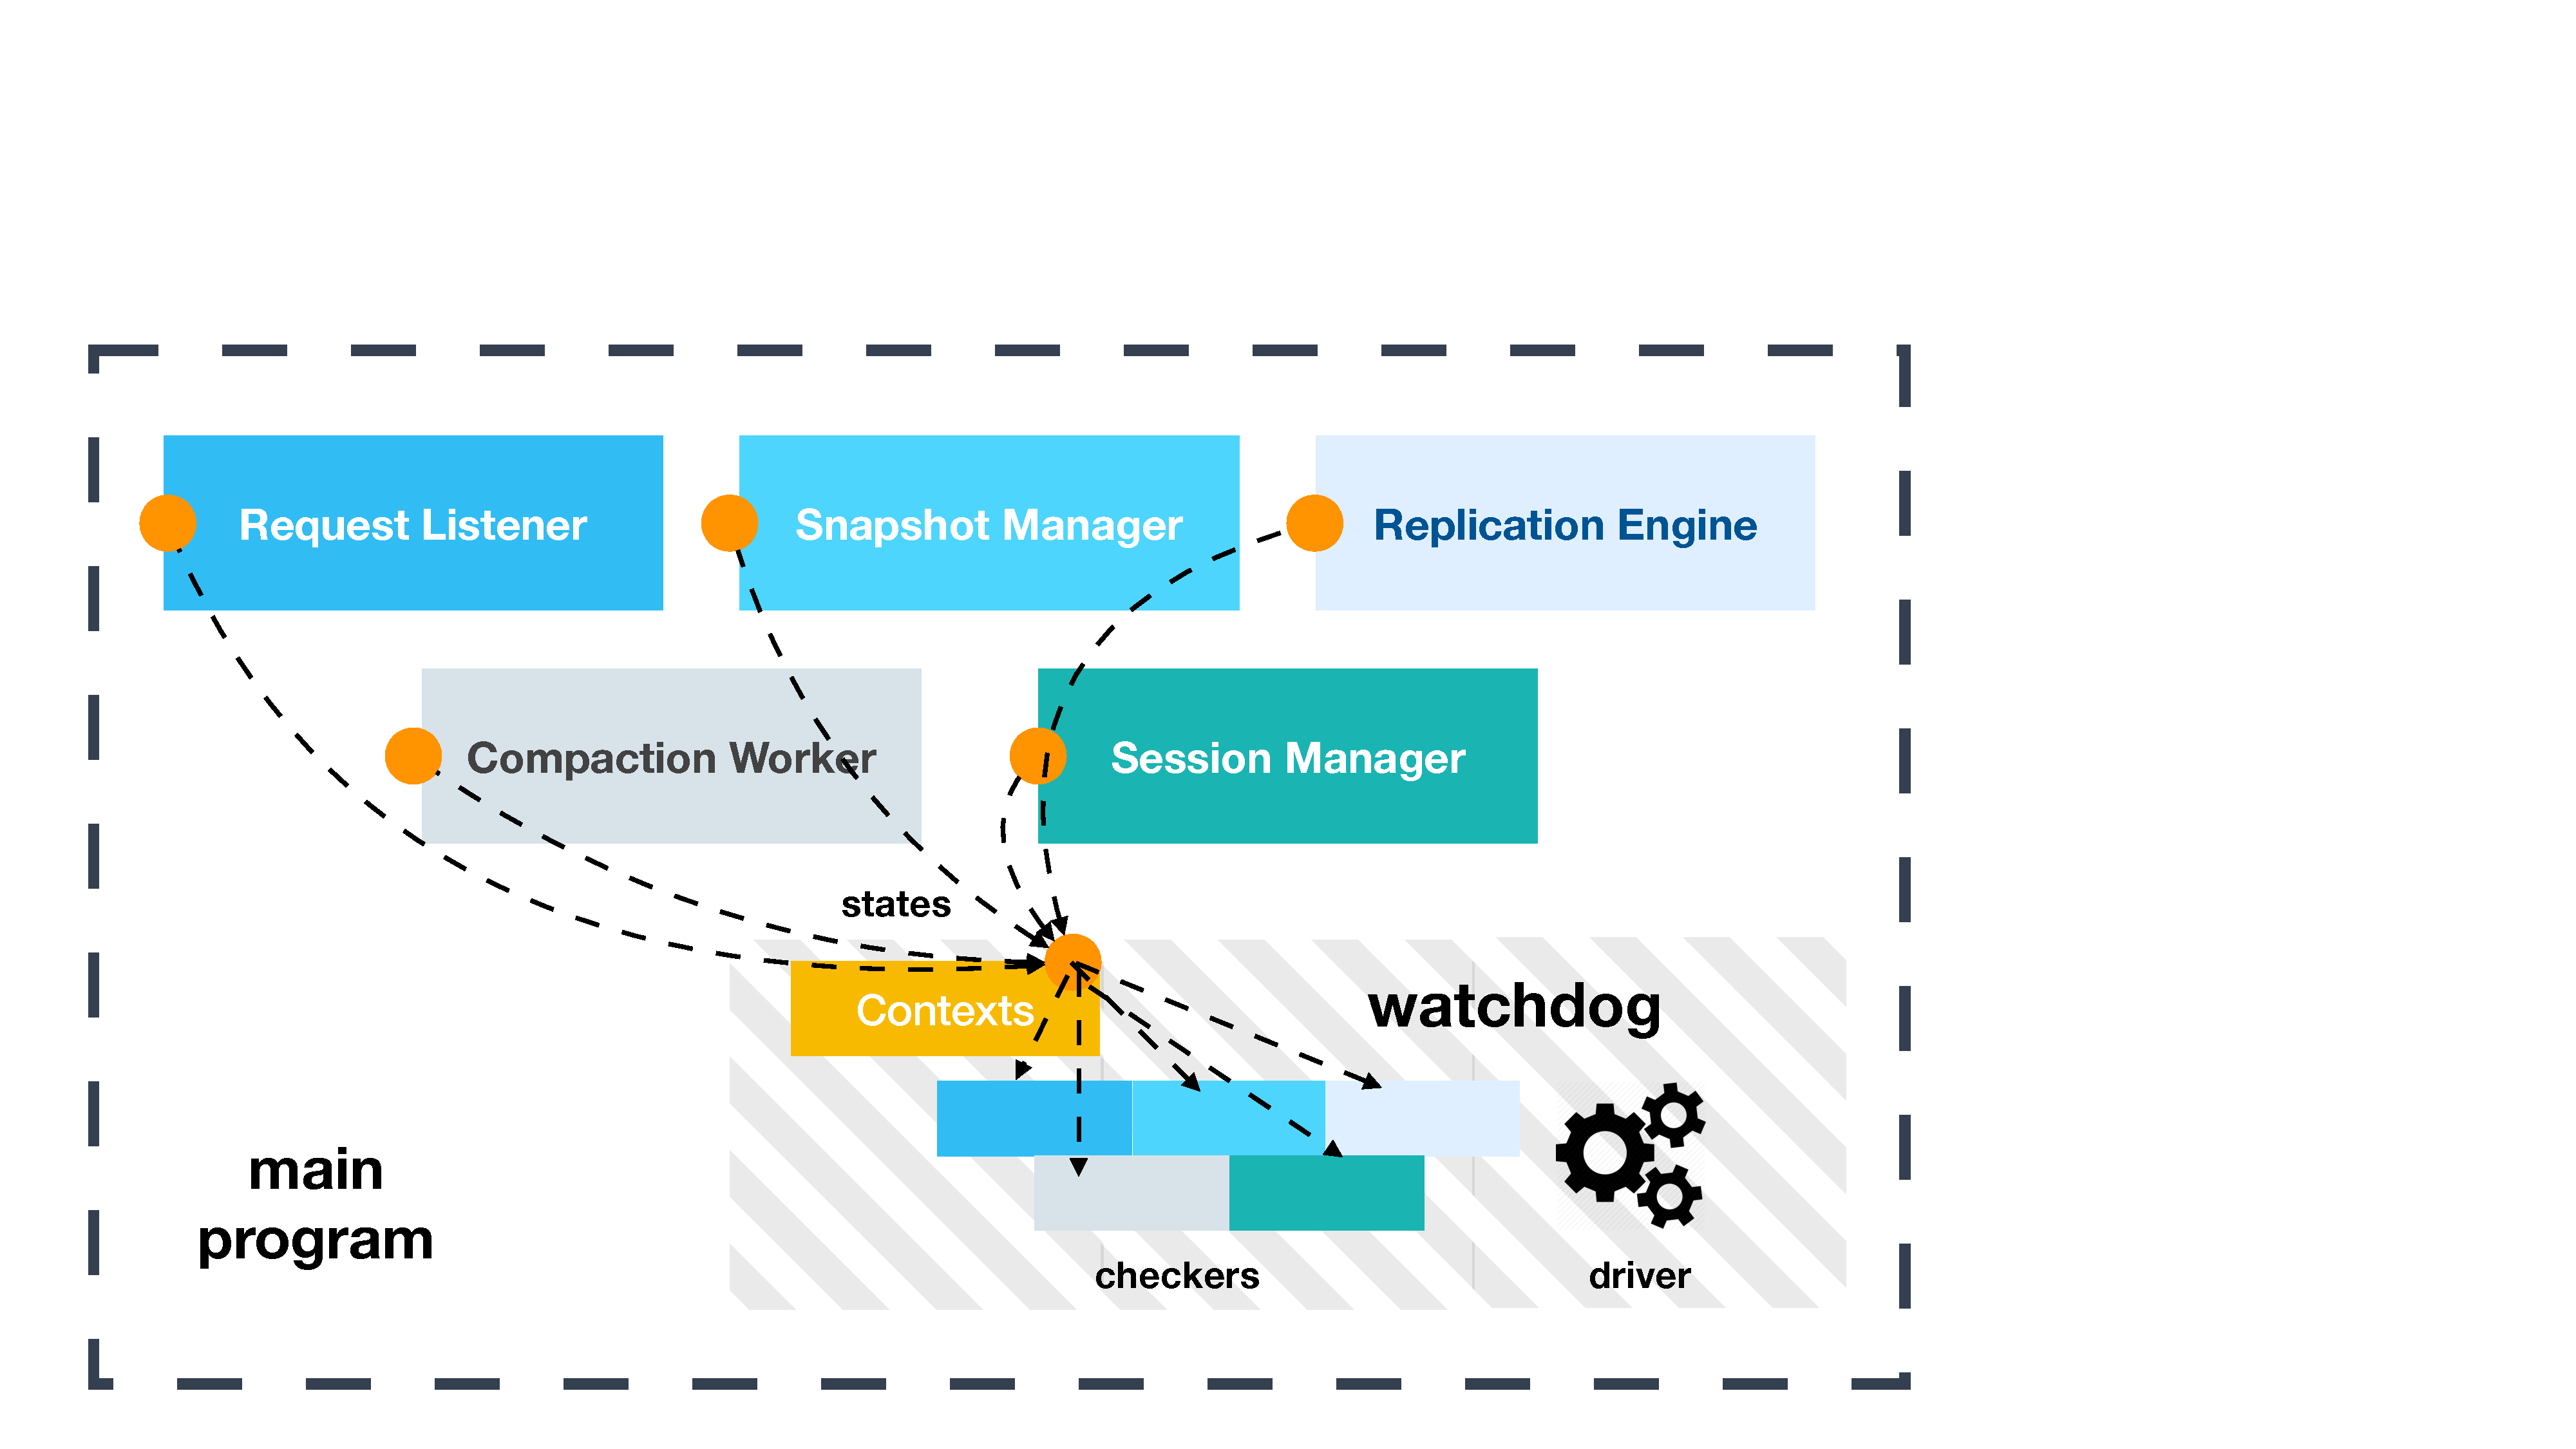
\includegraphics[width=\textwidth]{fig/staetful}
            \end{center}

            \textbf{Note:} The watchdog driver will not execute a checker unless its context is ready.

        \end{column}
    \end{columns}

\end{frame}

\begin{frame}{Characteristic III: Concurrent}
    Run watchdog \red{concurrently} with the main program instead of \blue{in-place} checking with \blue{inserted} checkers
    \begin{center}
        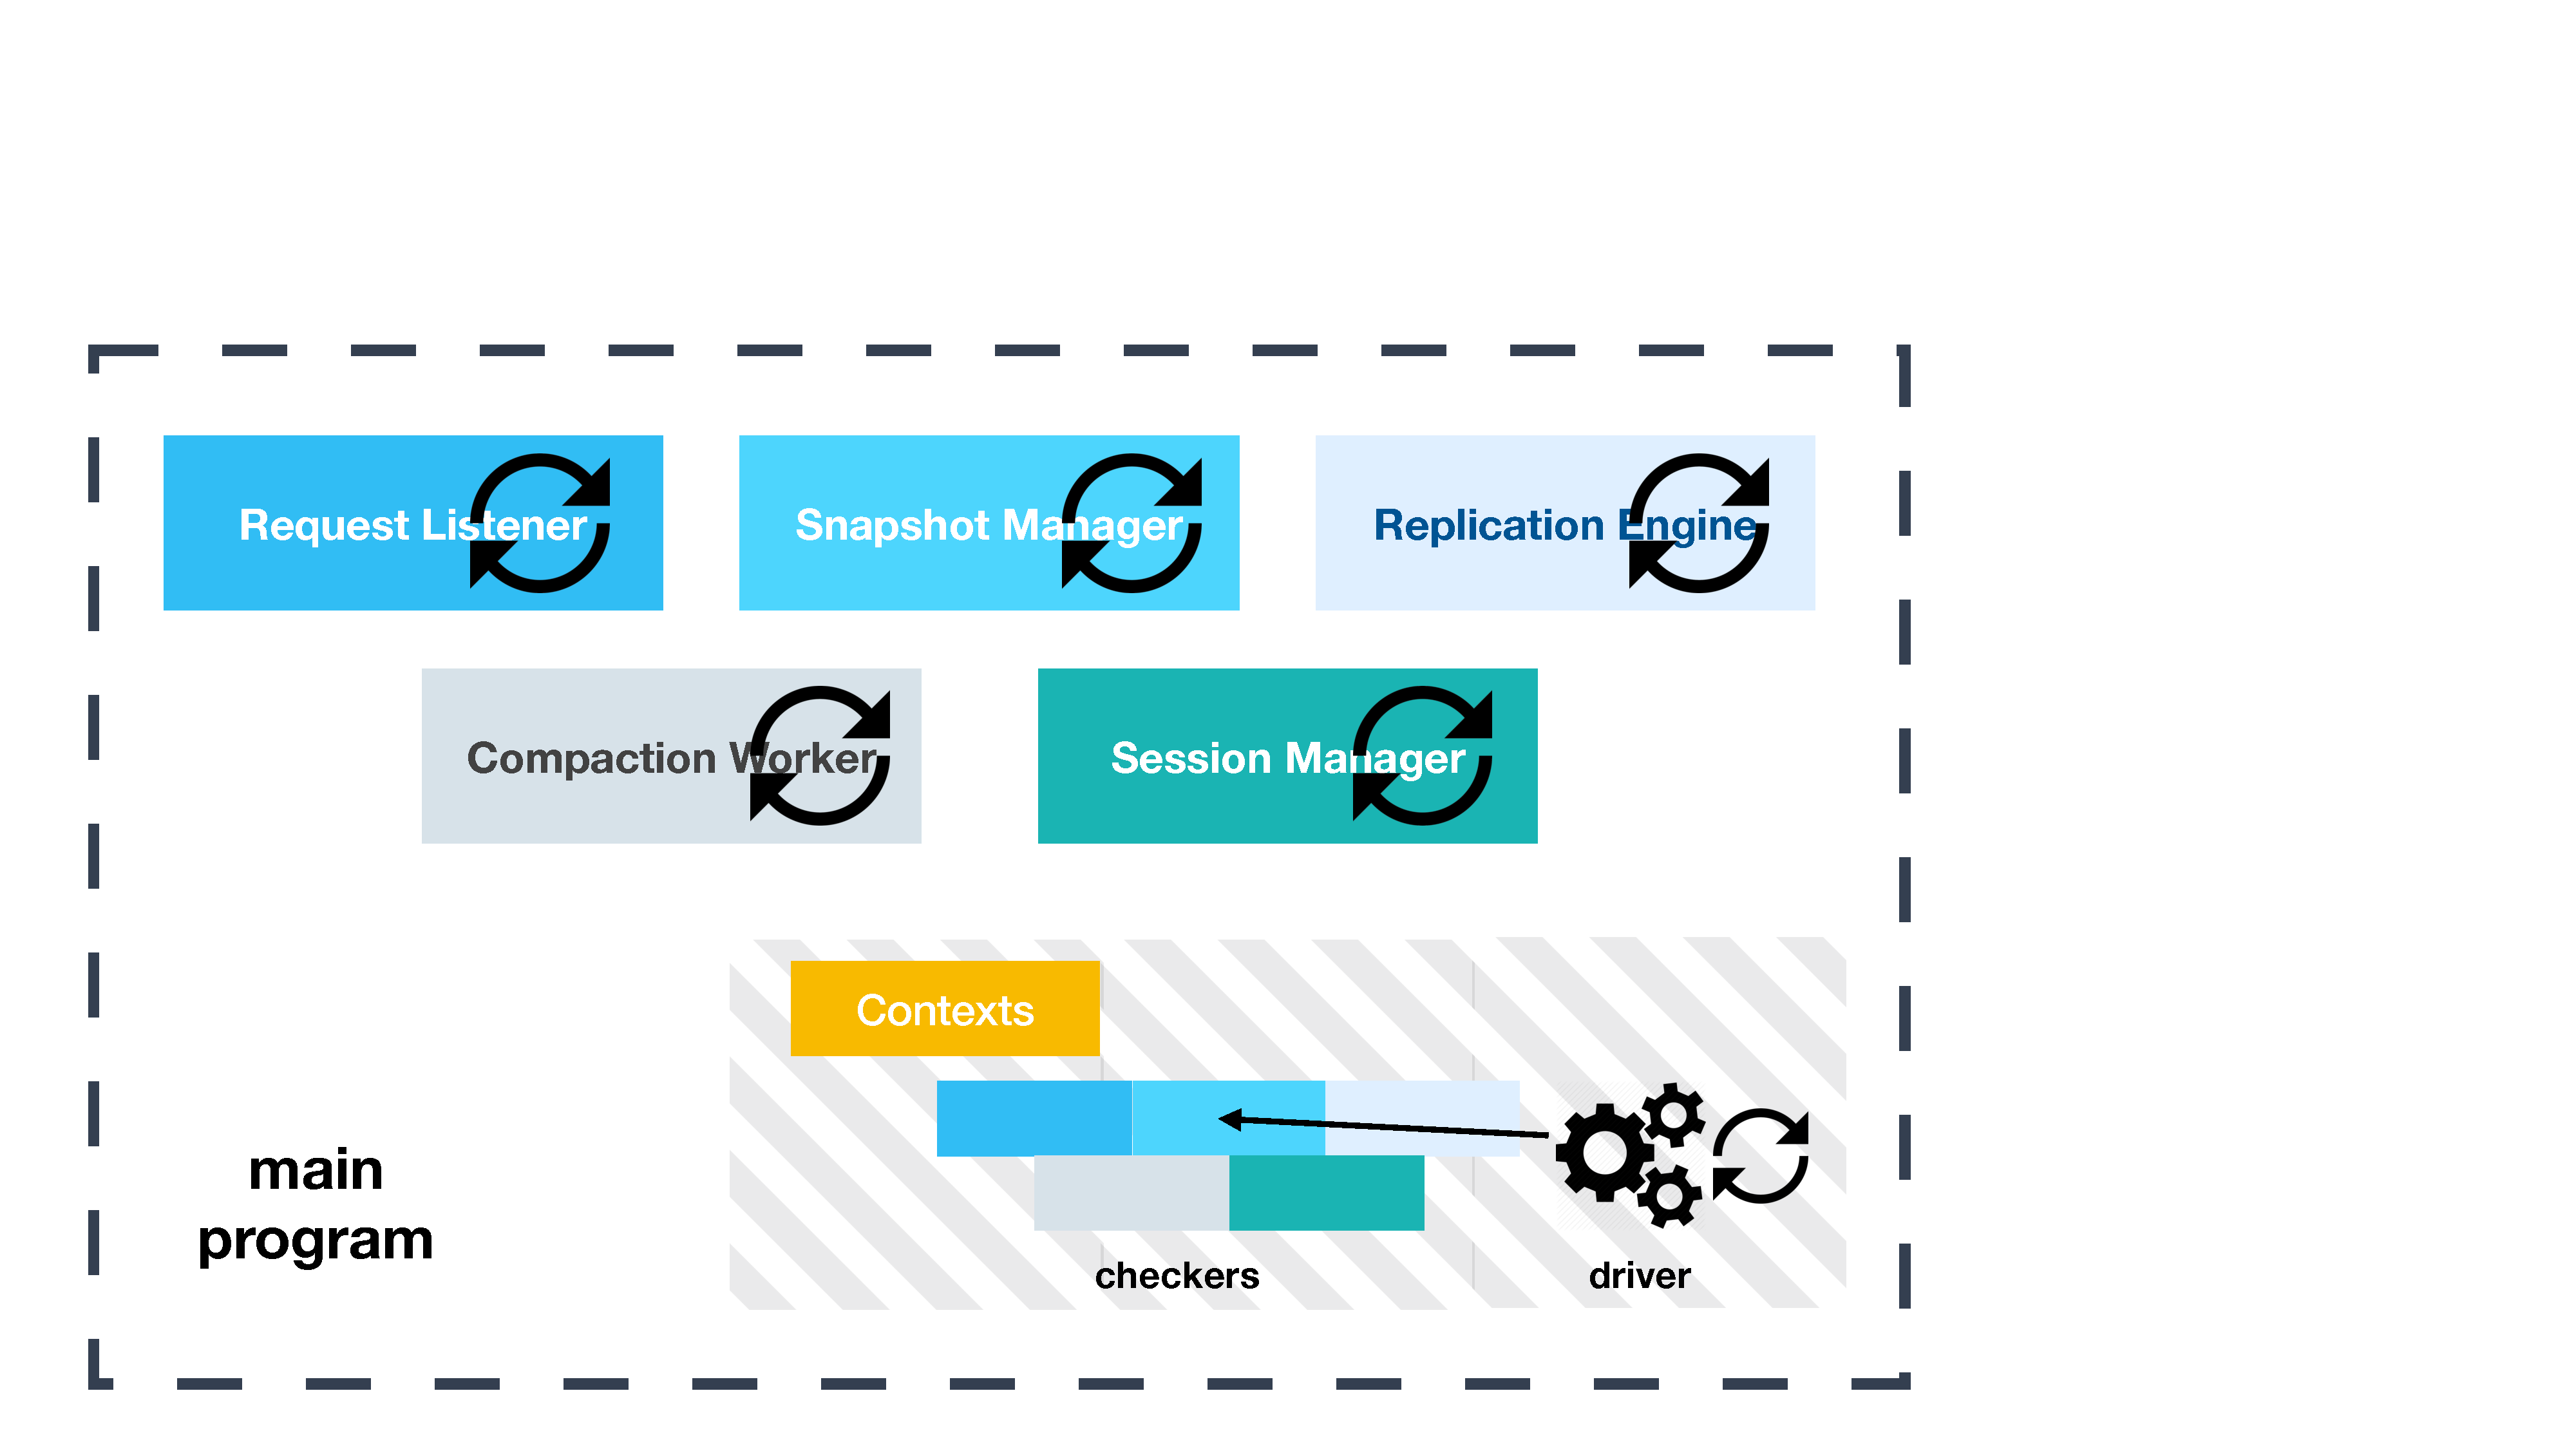
\includegraphics[width=.75
            \textwidth]{fig/concurrent}
    \end{center}
\end{frame}

\begin{frame}{Core Idea: Mimic Checking}
    \begin{columns}
        \begin{column}{.6\textwidth}
            Imitates some representative operations
            \begin{center}
                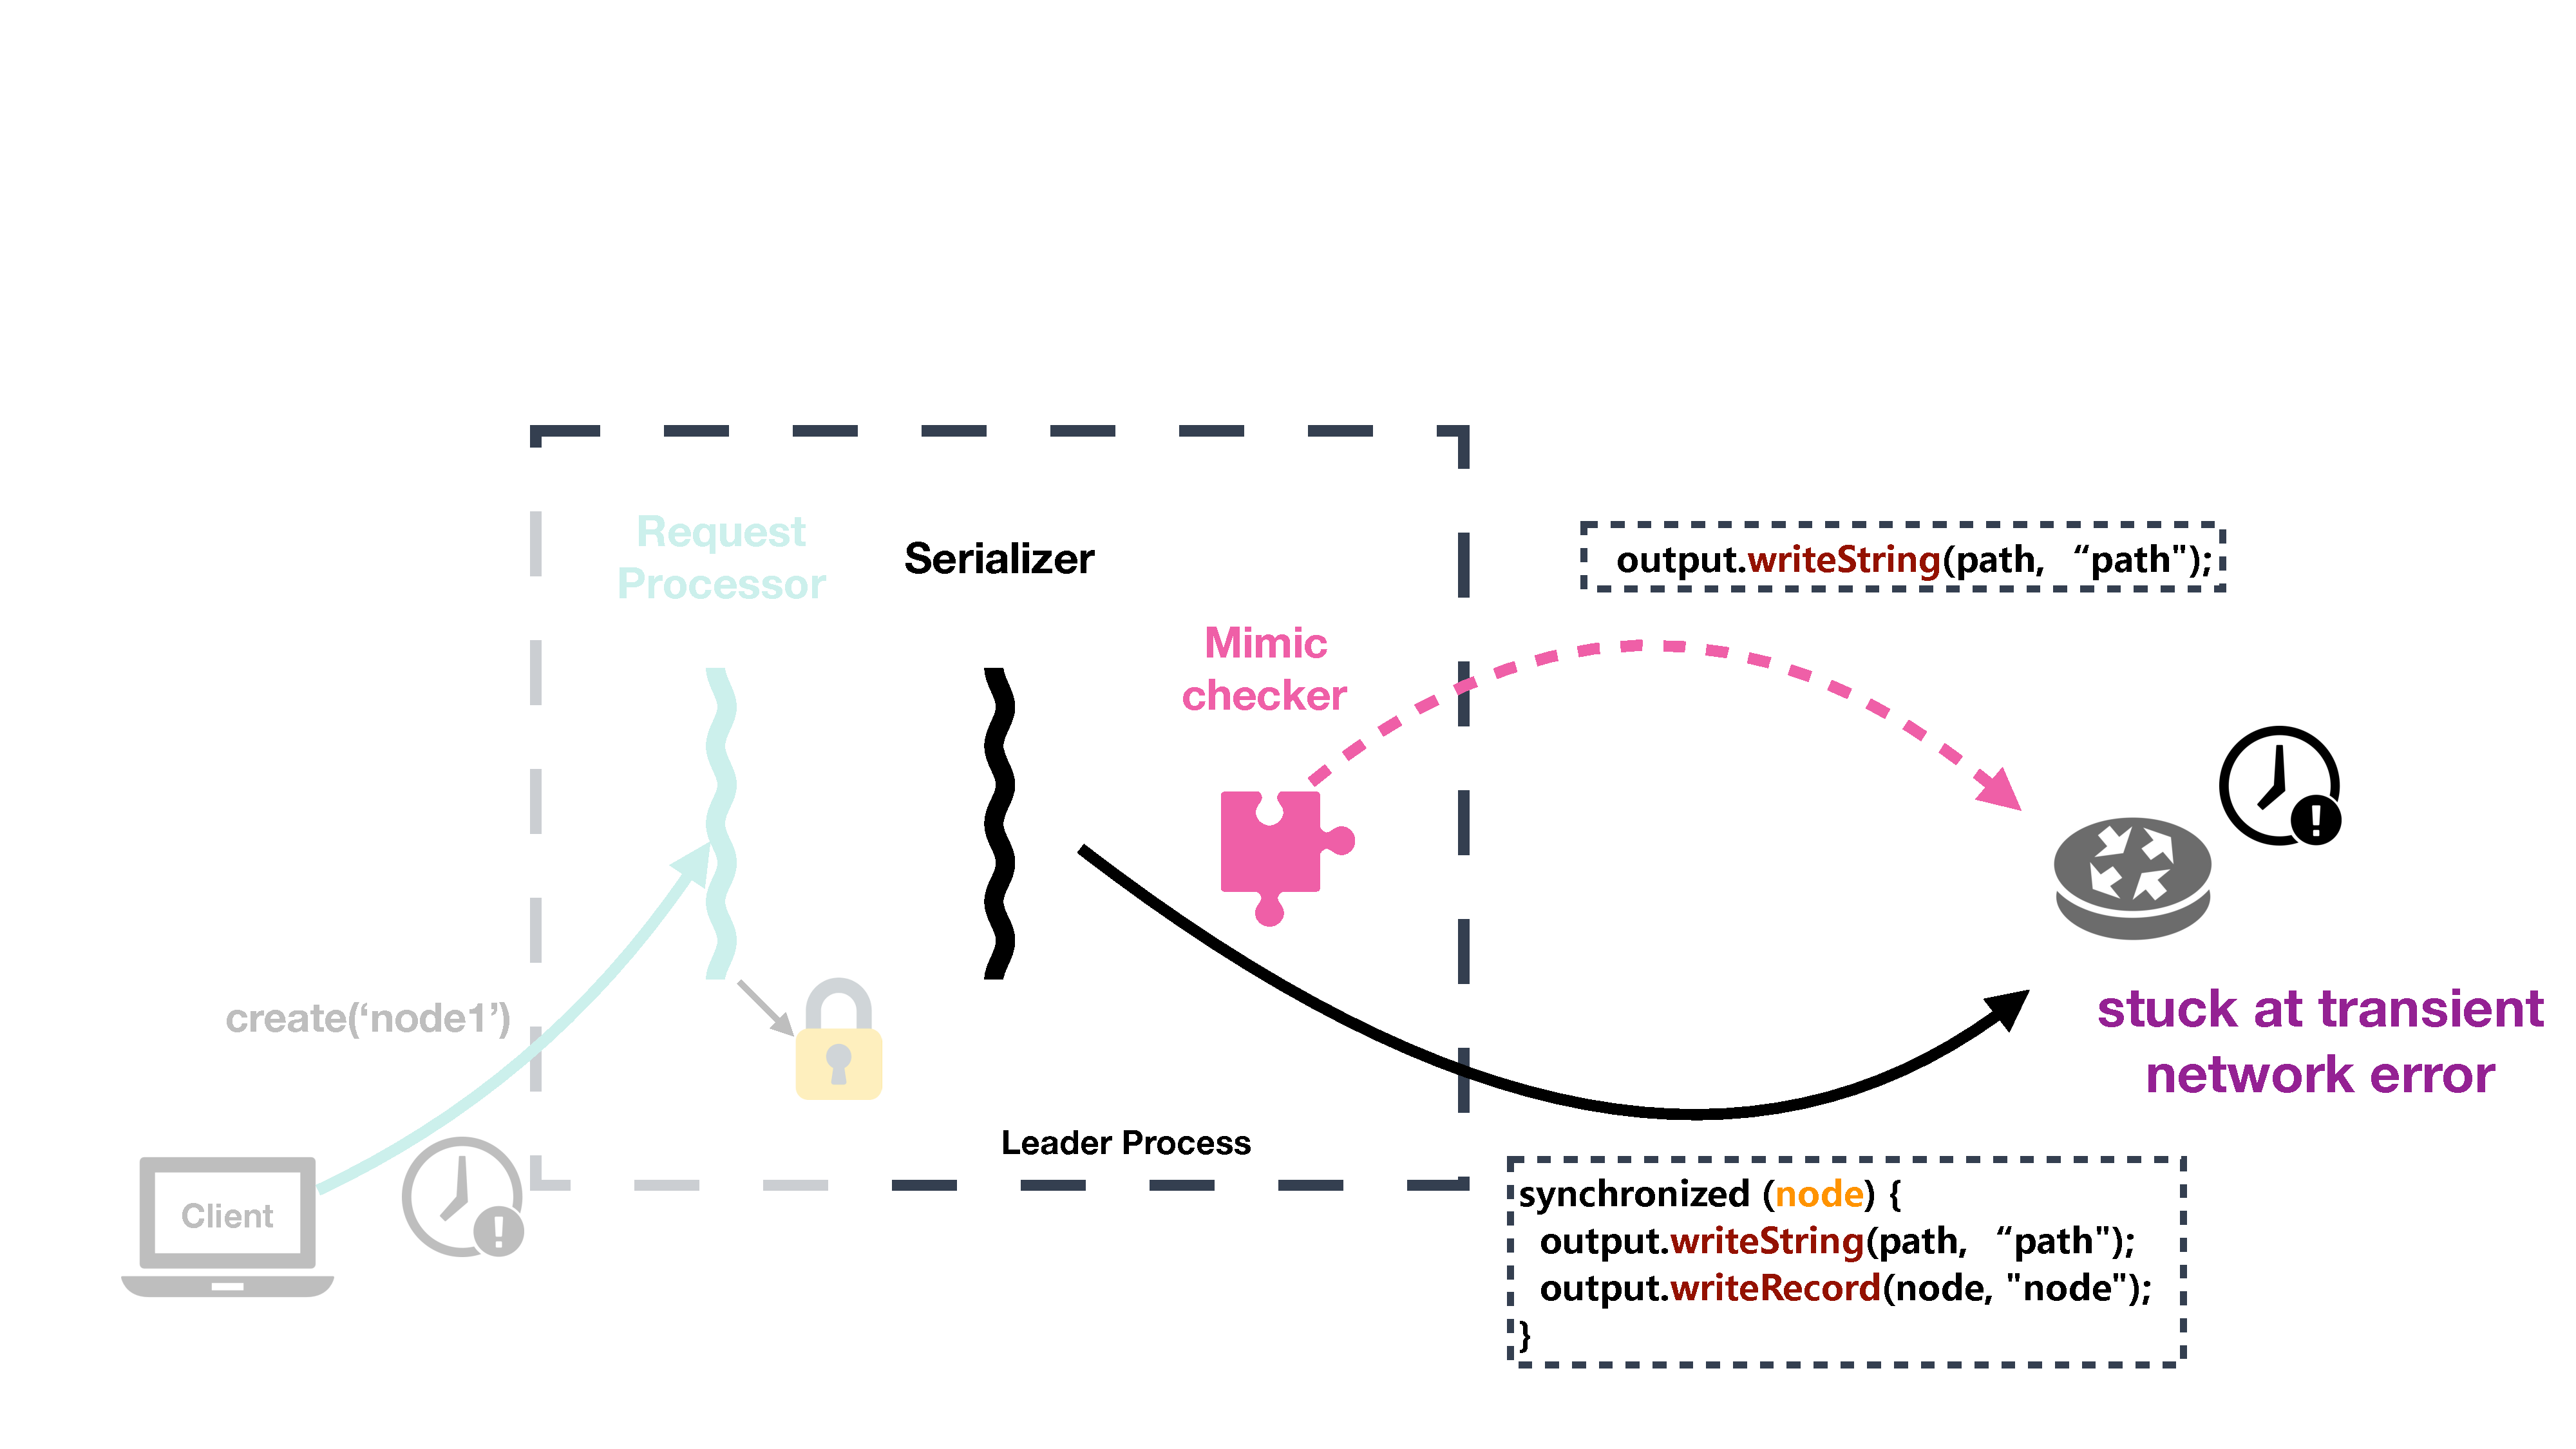
\includegraphics[width=\textwidth]{fig/mimic}
            \end{center}
            \textbf{Exmaple:} Perform a similar operation (snapshot) and also get stuck at the same location
        \end{column}

        \begin{column}{.4\textwidth}
            \begin{block}{\textbf{Accurancy}}
                \begin{itemize}
                    \item exercises code logic similar to the main program
                    \item share execution environment in runtime
                    \item increases coverage of checking targets
                    \item can pinpoint the faulty module and failing instruction
                \end{itemize}
            \end{block}
        \end{column}
    \end{columns}

\end{frame}

\subsection{Implementation}

\begin{frame}[fragile]{Implementation: \texttt{OmegaGen}}
    \framesubtitle{Tool Overview}

    \begin{itemize}
        \item a prototype that systematically generates mimic-type watchdogs for system softwares
        \item in Java with 8,100 SLOC, using  \texttt{Soot} analysis framework
        \item \textbf{core technique:} \red{program reduction}

    \end{itemize}

    \begin{lstlisting}[language=sh]
$ ./omegagen -jar zookeeper-3.4.6.jar -m zookeeper.manifest
analyzing..
generating..
instrumenting..
repackaging..
done. Total 1min 6s.
$ ls output/
zookeeper-3.4.6-with-wd.jar
\end{lstlisting}

\end{frame}

\begin{frame}{What is Program Reduction?}
    \begin{definition}
        Given a program \red{$P$}, create a watchdog \blue{$W$} that can detect partial failures in \red{$P$} without imposing on \red{$P$}’s execution.
    \end{definition}

    \begin{center}
        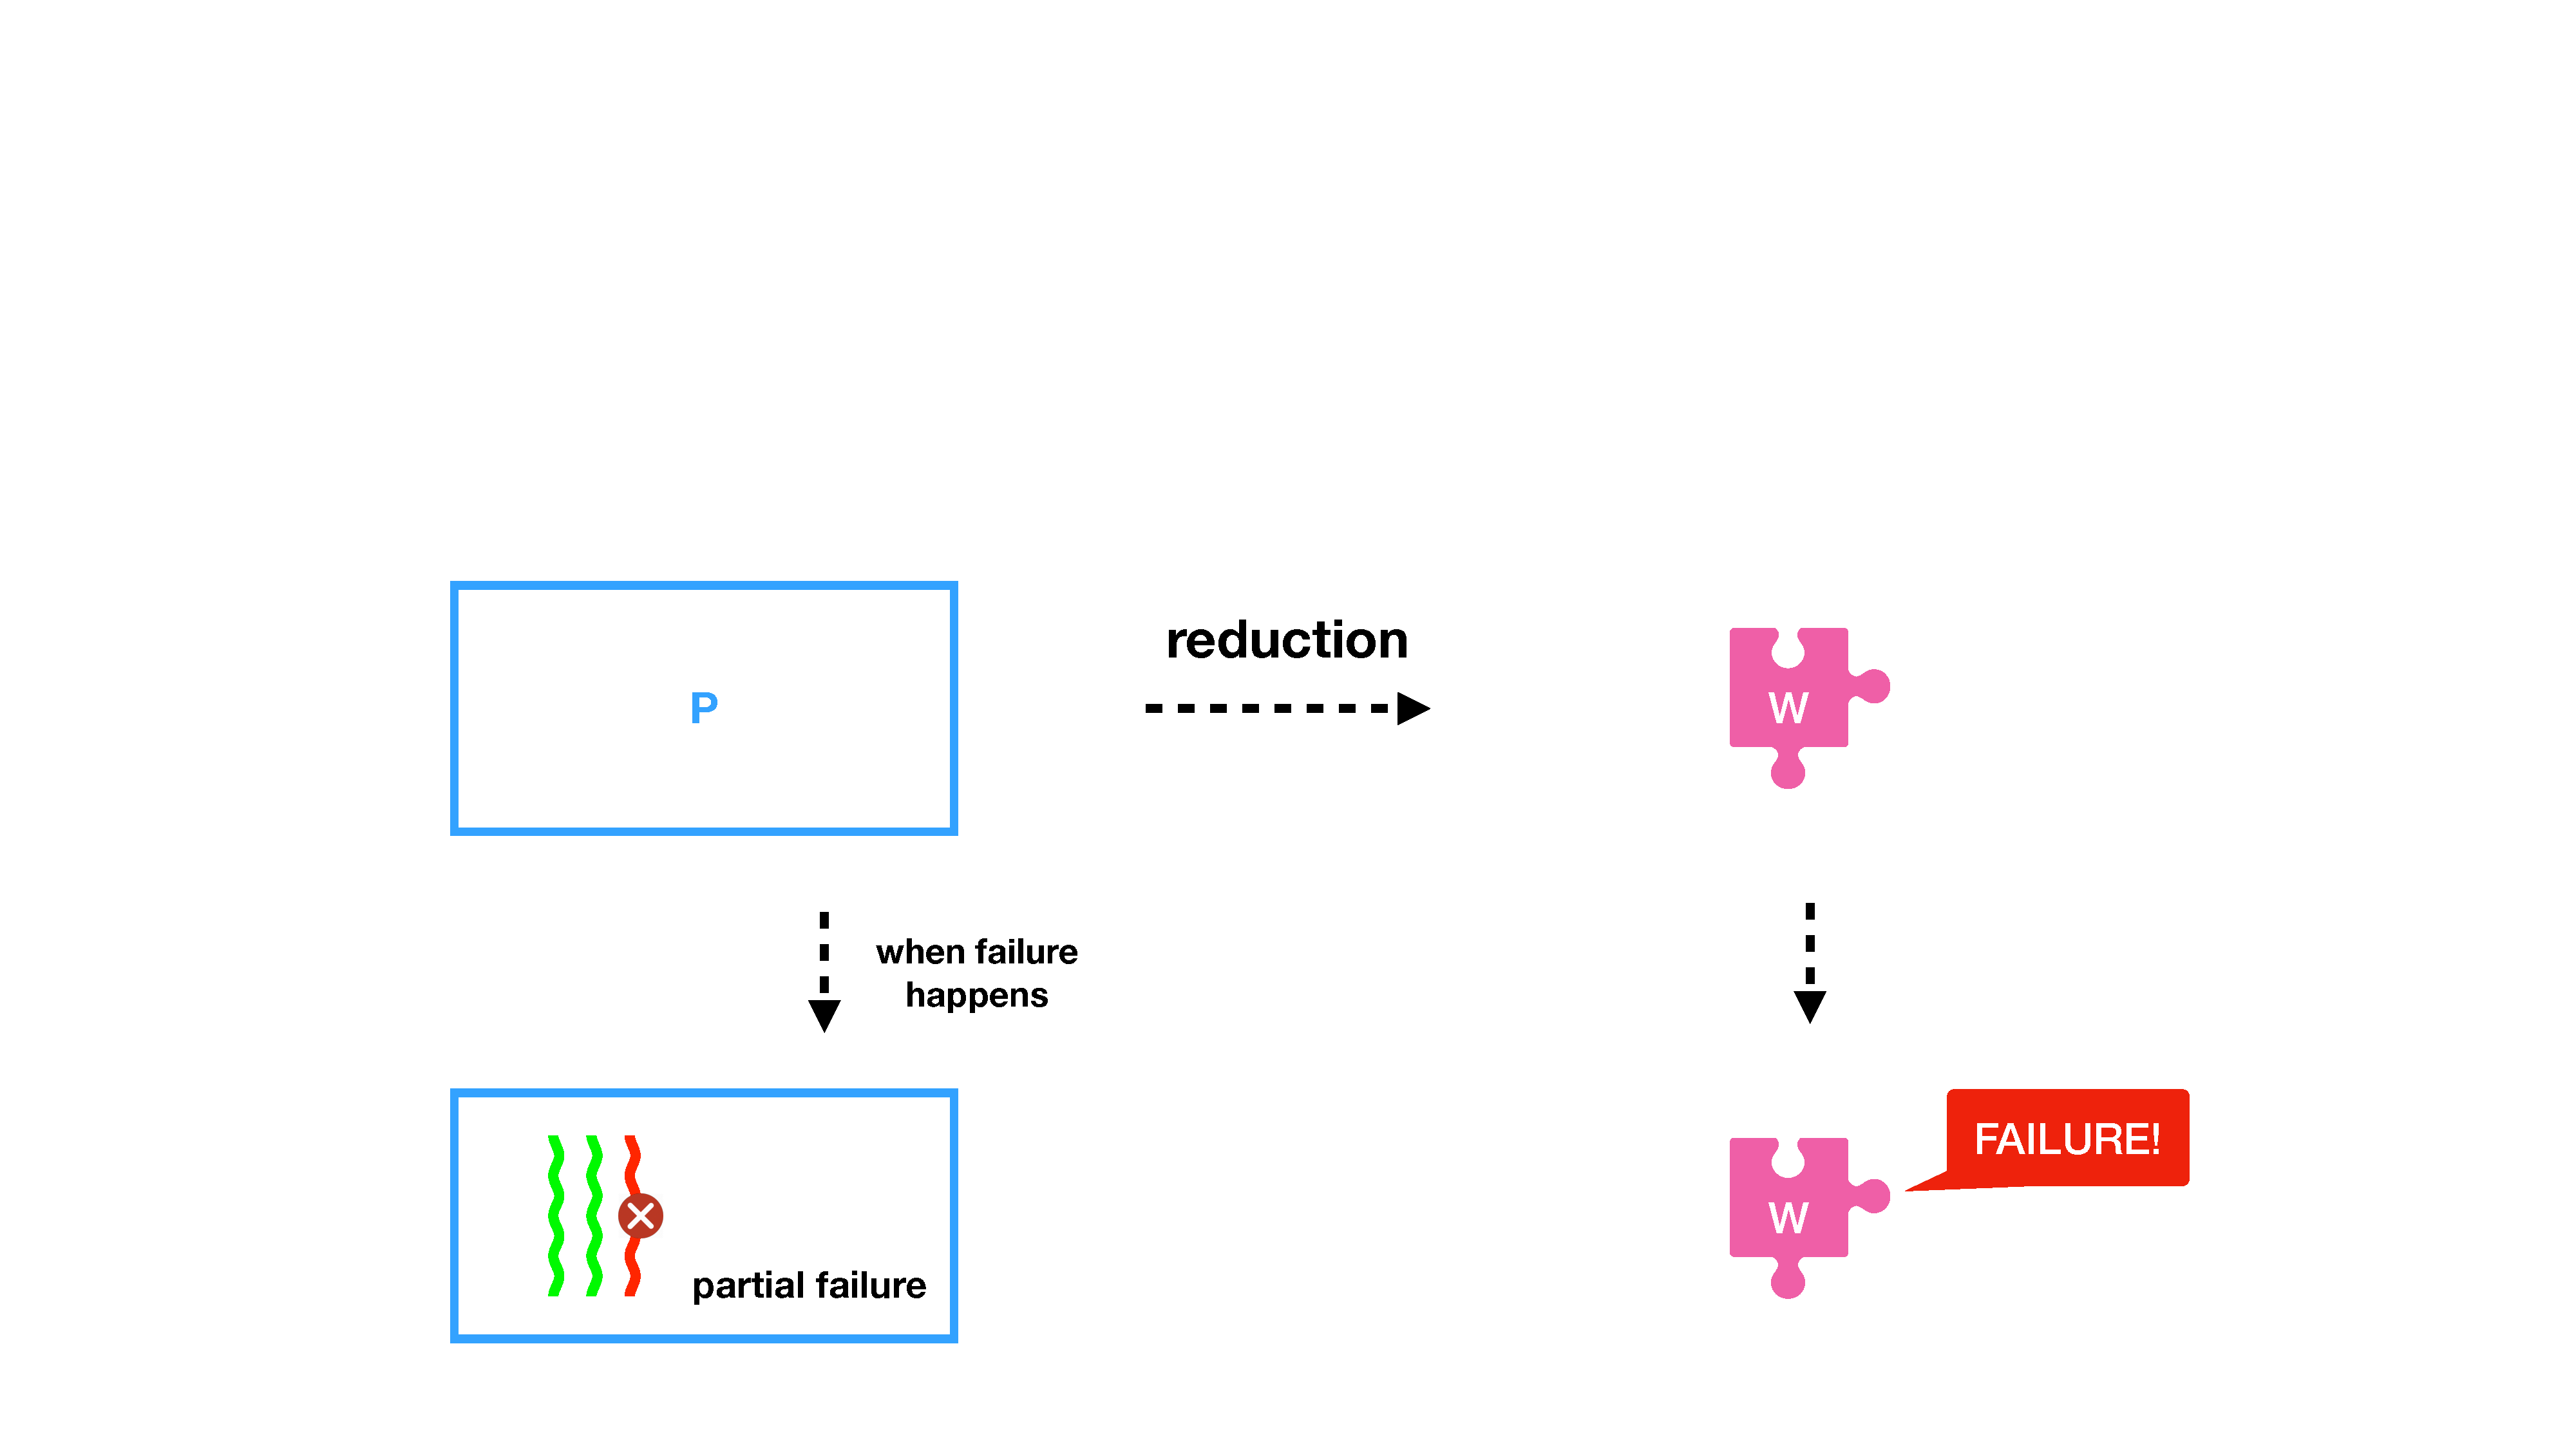
\includegraphics[width=.6\textwidth]{fig/reduce}
    \end{center}

    \textbf{Reduce:} We need not put everything into checkers, because a lot of operations are logically \red{deterministic} and should be checked before production. Only some of them are more \red{vulnerable}
    in the production environment.
\end{frame}

\begin{frame}{Program Reduction}
    For the source code of a given program, the process will go through five steps:
    \vspace{2em}
    \begin{enumerate}
        \item locate long-running regions
        \item  reduce the program
        \item  locate vulnerable operations
        \item  encapsulate watchdog checkers
        \item  insert watchdog hooks
    \end{enumerate}
\end{frame}

\begin{frame}{Step 1: Locate Long-running Regions}
    \begin{block}{Identifies potentially long-running loops in the function body}
        e.g. \texttt{while(true)},\texttt{while(flag)}
    \end{block}

    However, an identified \red{long-running} loop may turn out to be \blue{short-lived} in an actual run.

    \begin{block}{\textbf{predicate}-based algorithm}
        a runtime property associated with a method which tracks whether a call site of this method is in fact reached
        \begin{itemize}
            \item insert a hook before the loop $\to$  sets its predicate
            \item insert a hook after the loop $\to$ unset its predicate
            \item pass caller’s predicate set to callees
        \end{itemize}
        Runtime:
        \begin{itemize}
            \item activate or activates or deactivates the associated watchdog based on assigned predicate
        \end{itemize}
    \end{block}

\end{frame}

\begin{frame}{Step 1: Locate Long-running Regions}
    \framesubtitle{An example}
    \begin{center}
        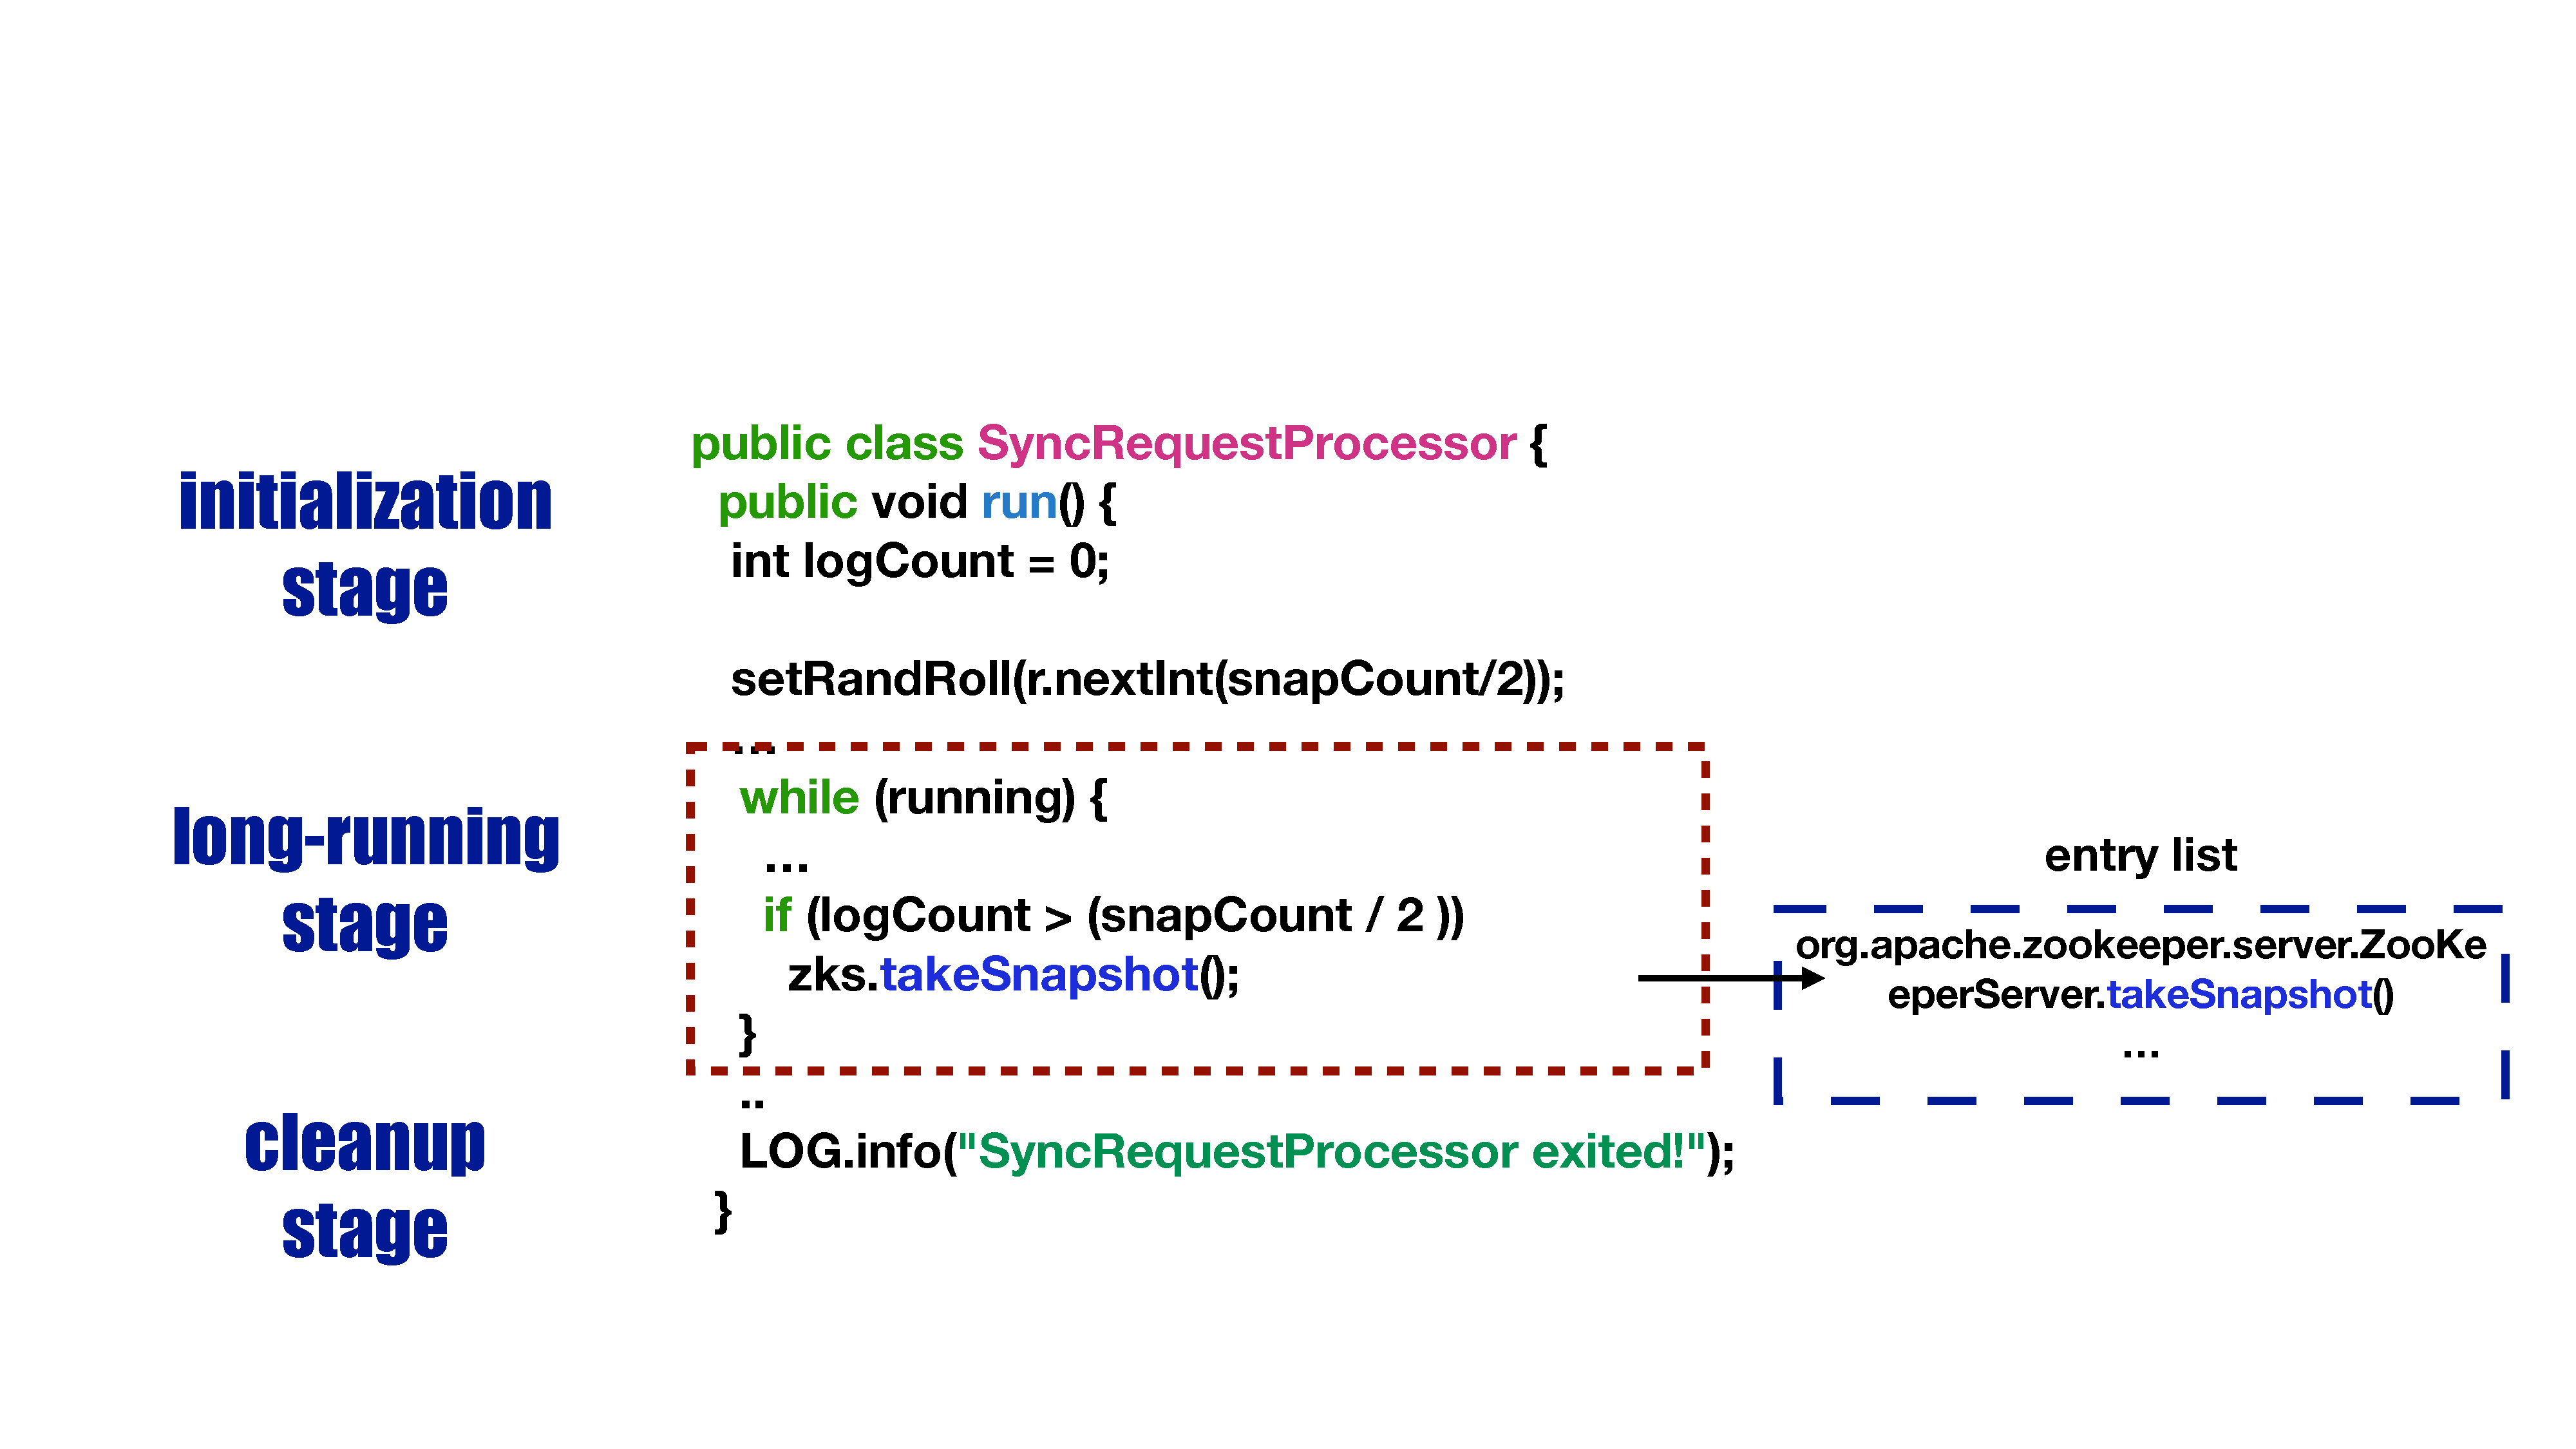
\includegraphics[width=.9\textwidth]{fig/long-run}
    \end{center}
\end{frame}

\begin{frame}{Step 2: Reduce the Program}
    Recursively analyze each function to find out \red{vulnerable} operations (in the next step)
    \begin{center}
        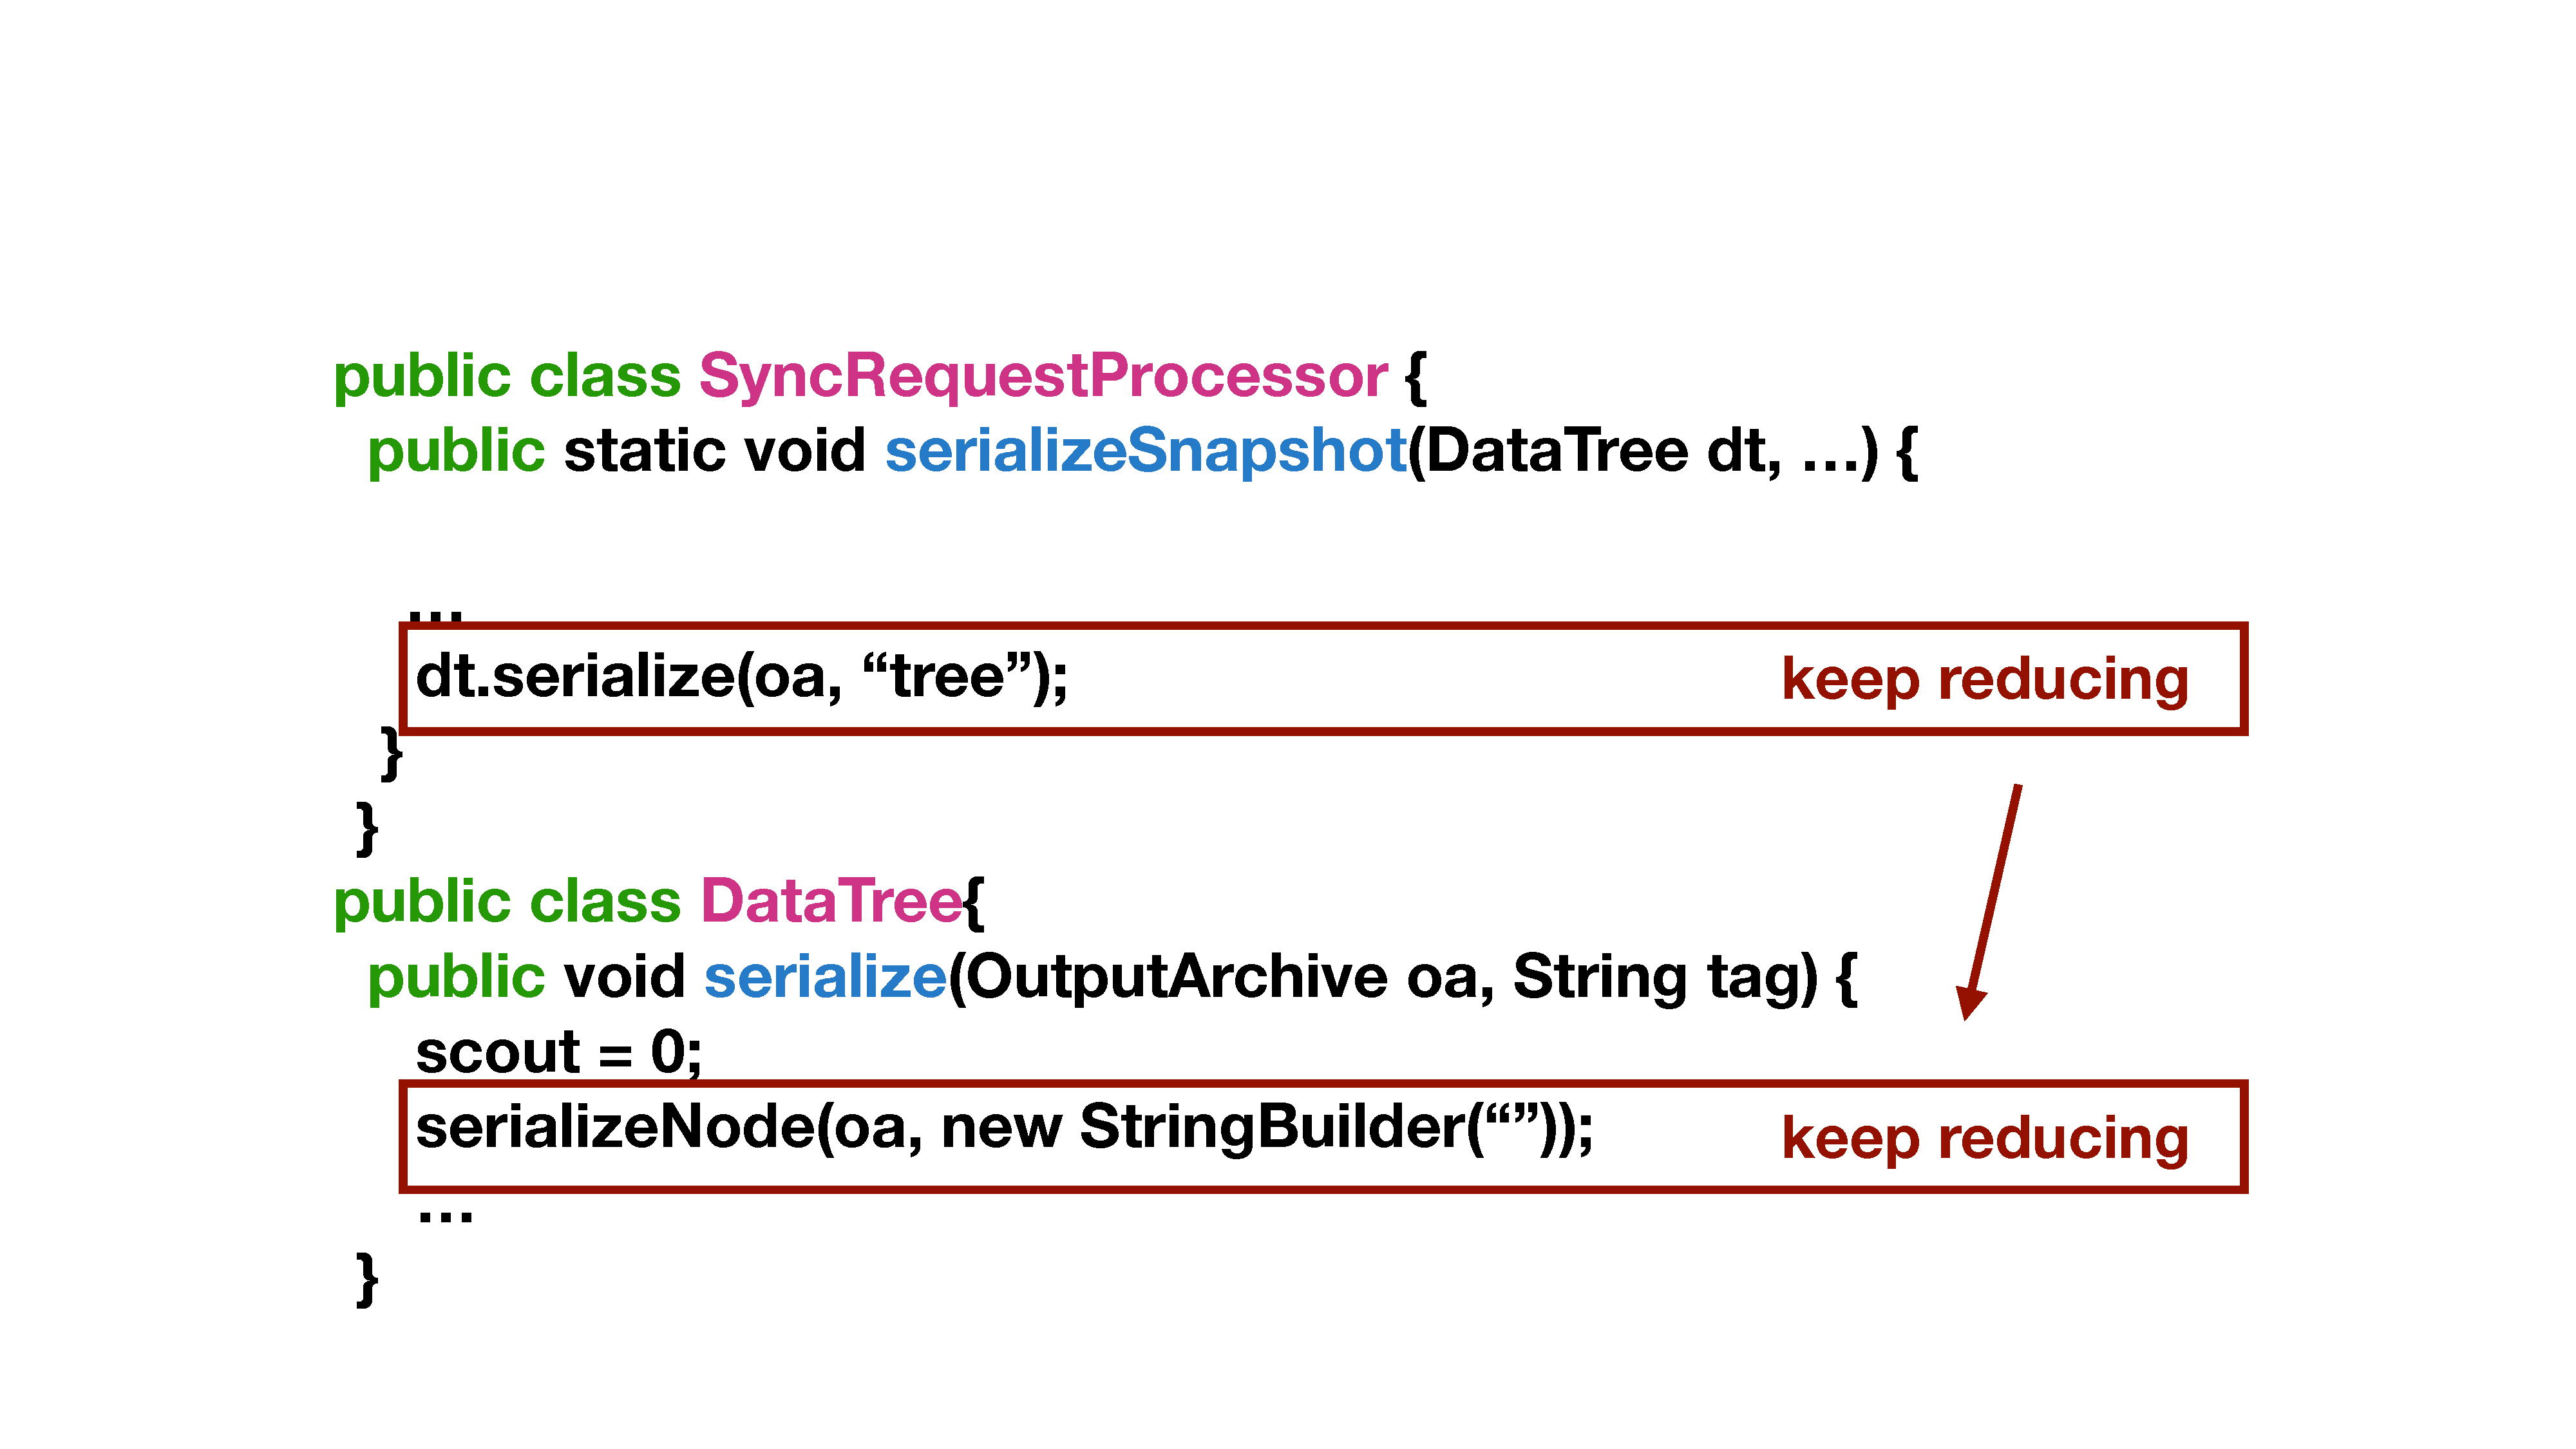
\includegraphics[width=.8\textwidth]{fig/rec-reduce}
    \end{center}
\end{frame}

\begin{frame}{Step 3: Locate Vulnerable Operations}
    Looks for potentially \red{vulnerable} operations in the control flow of those long-running methods.

    \begin{itemize}
        \item Heuristics (default):
              \begin{itemize}
                  \item synchronization
                  \item resource allocation
                  \item event polling
                  \item async waiting
                  \item invocations using external arguments
                  \item file or network I/
                  \item complex while loop conditional
              \end{itemize}
        \item Customize rule table in configuration
        \item Developers can also explicitly annotate an operation as \texttt{@vulnerable} in source codes
    \end{itemize}
\end{frame}

\begin{frame}{Step 4: Encapsulate Watchdog Checkers}
    \framesubtitle{Construct reduced method for each \red{vulnerable} method in main program}
    \begin{center}
        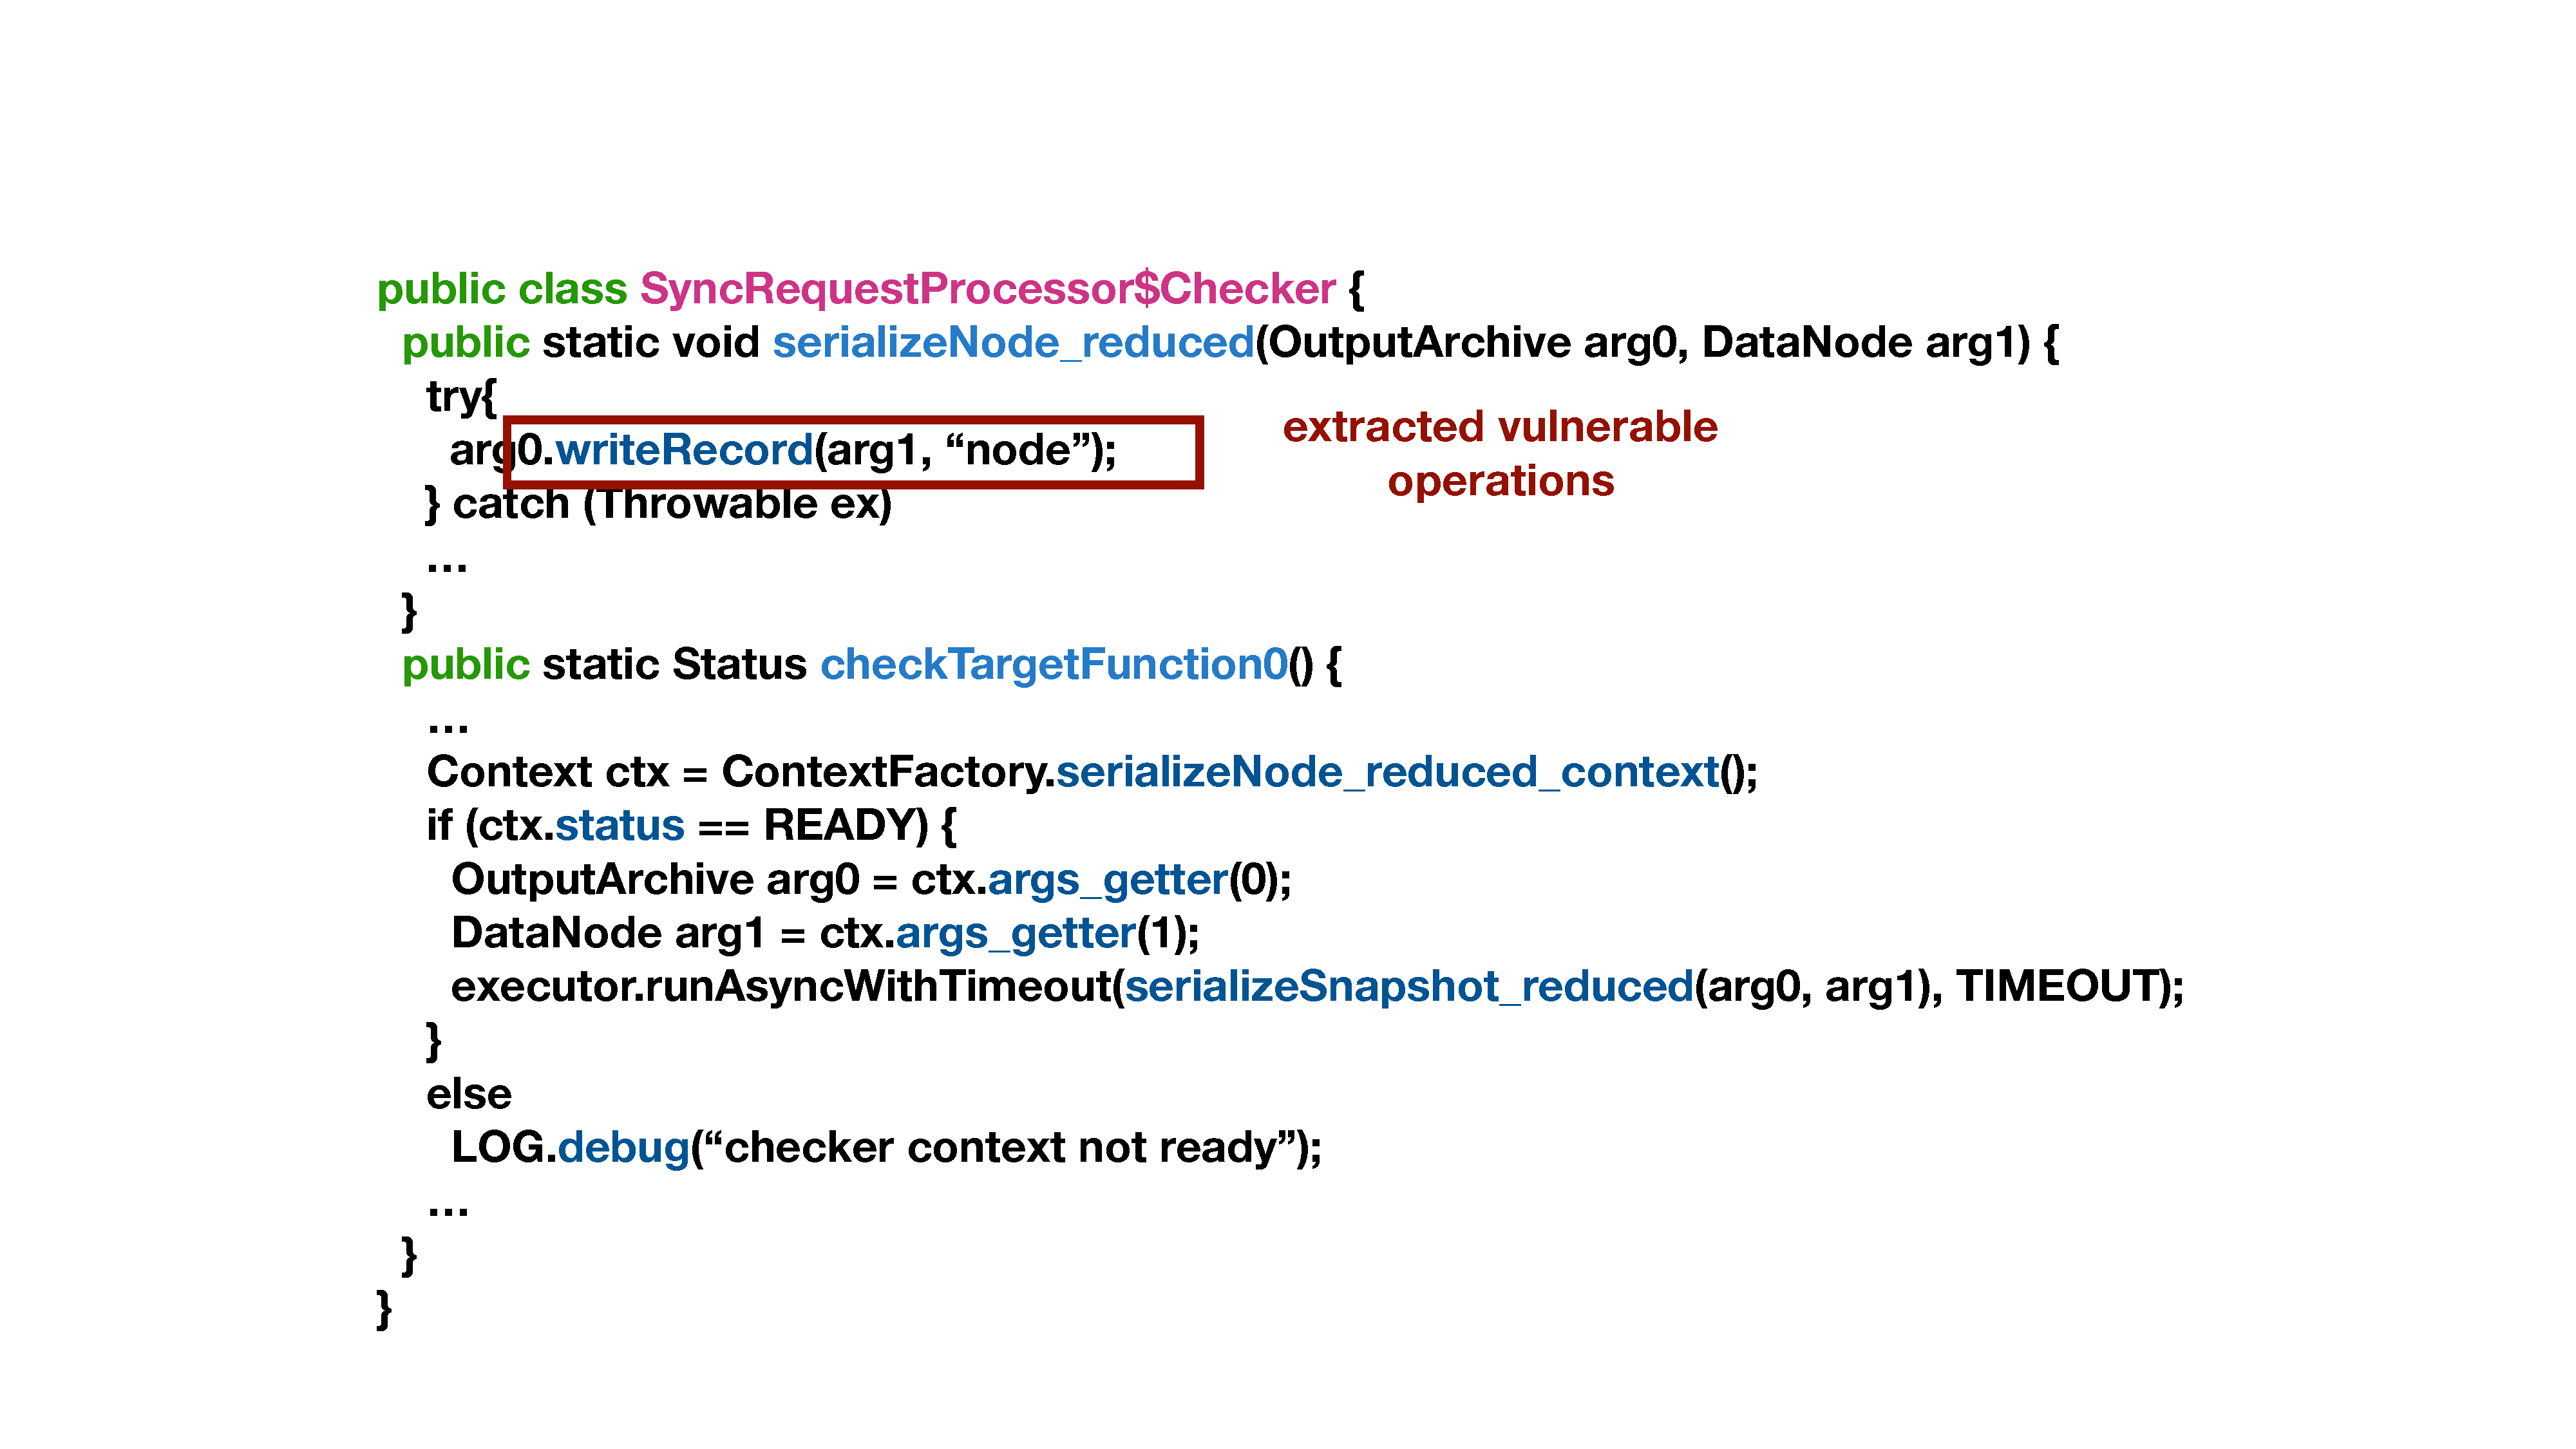
\includegraphics[width=.85\textwidth]{fig/encapsulate}
    \end{center}
\end{frame}

\begin{frame}{Step 5: Insert Watchdog Hooks}
    \framesubtitle{To capture the real state of the main program in runtime and pass it to the checker}
    \begin{center}
        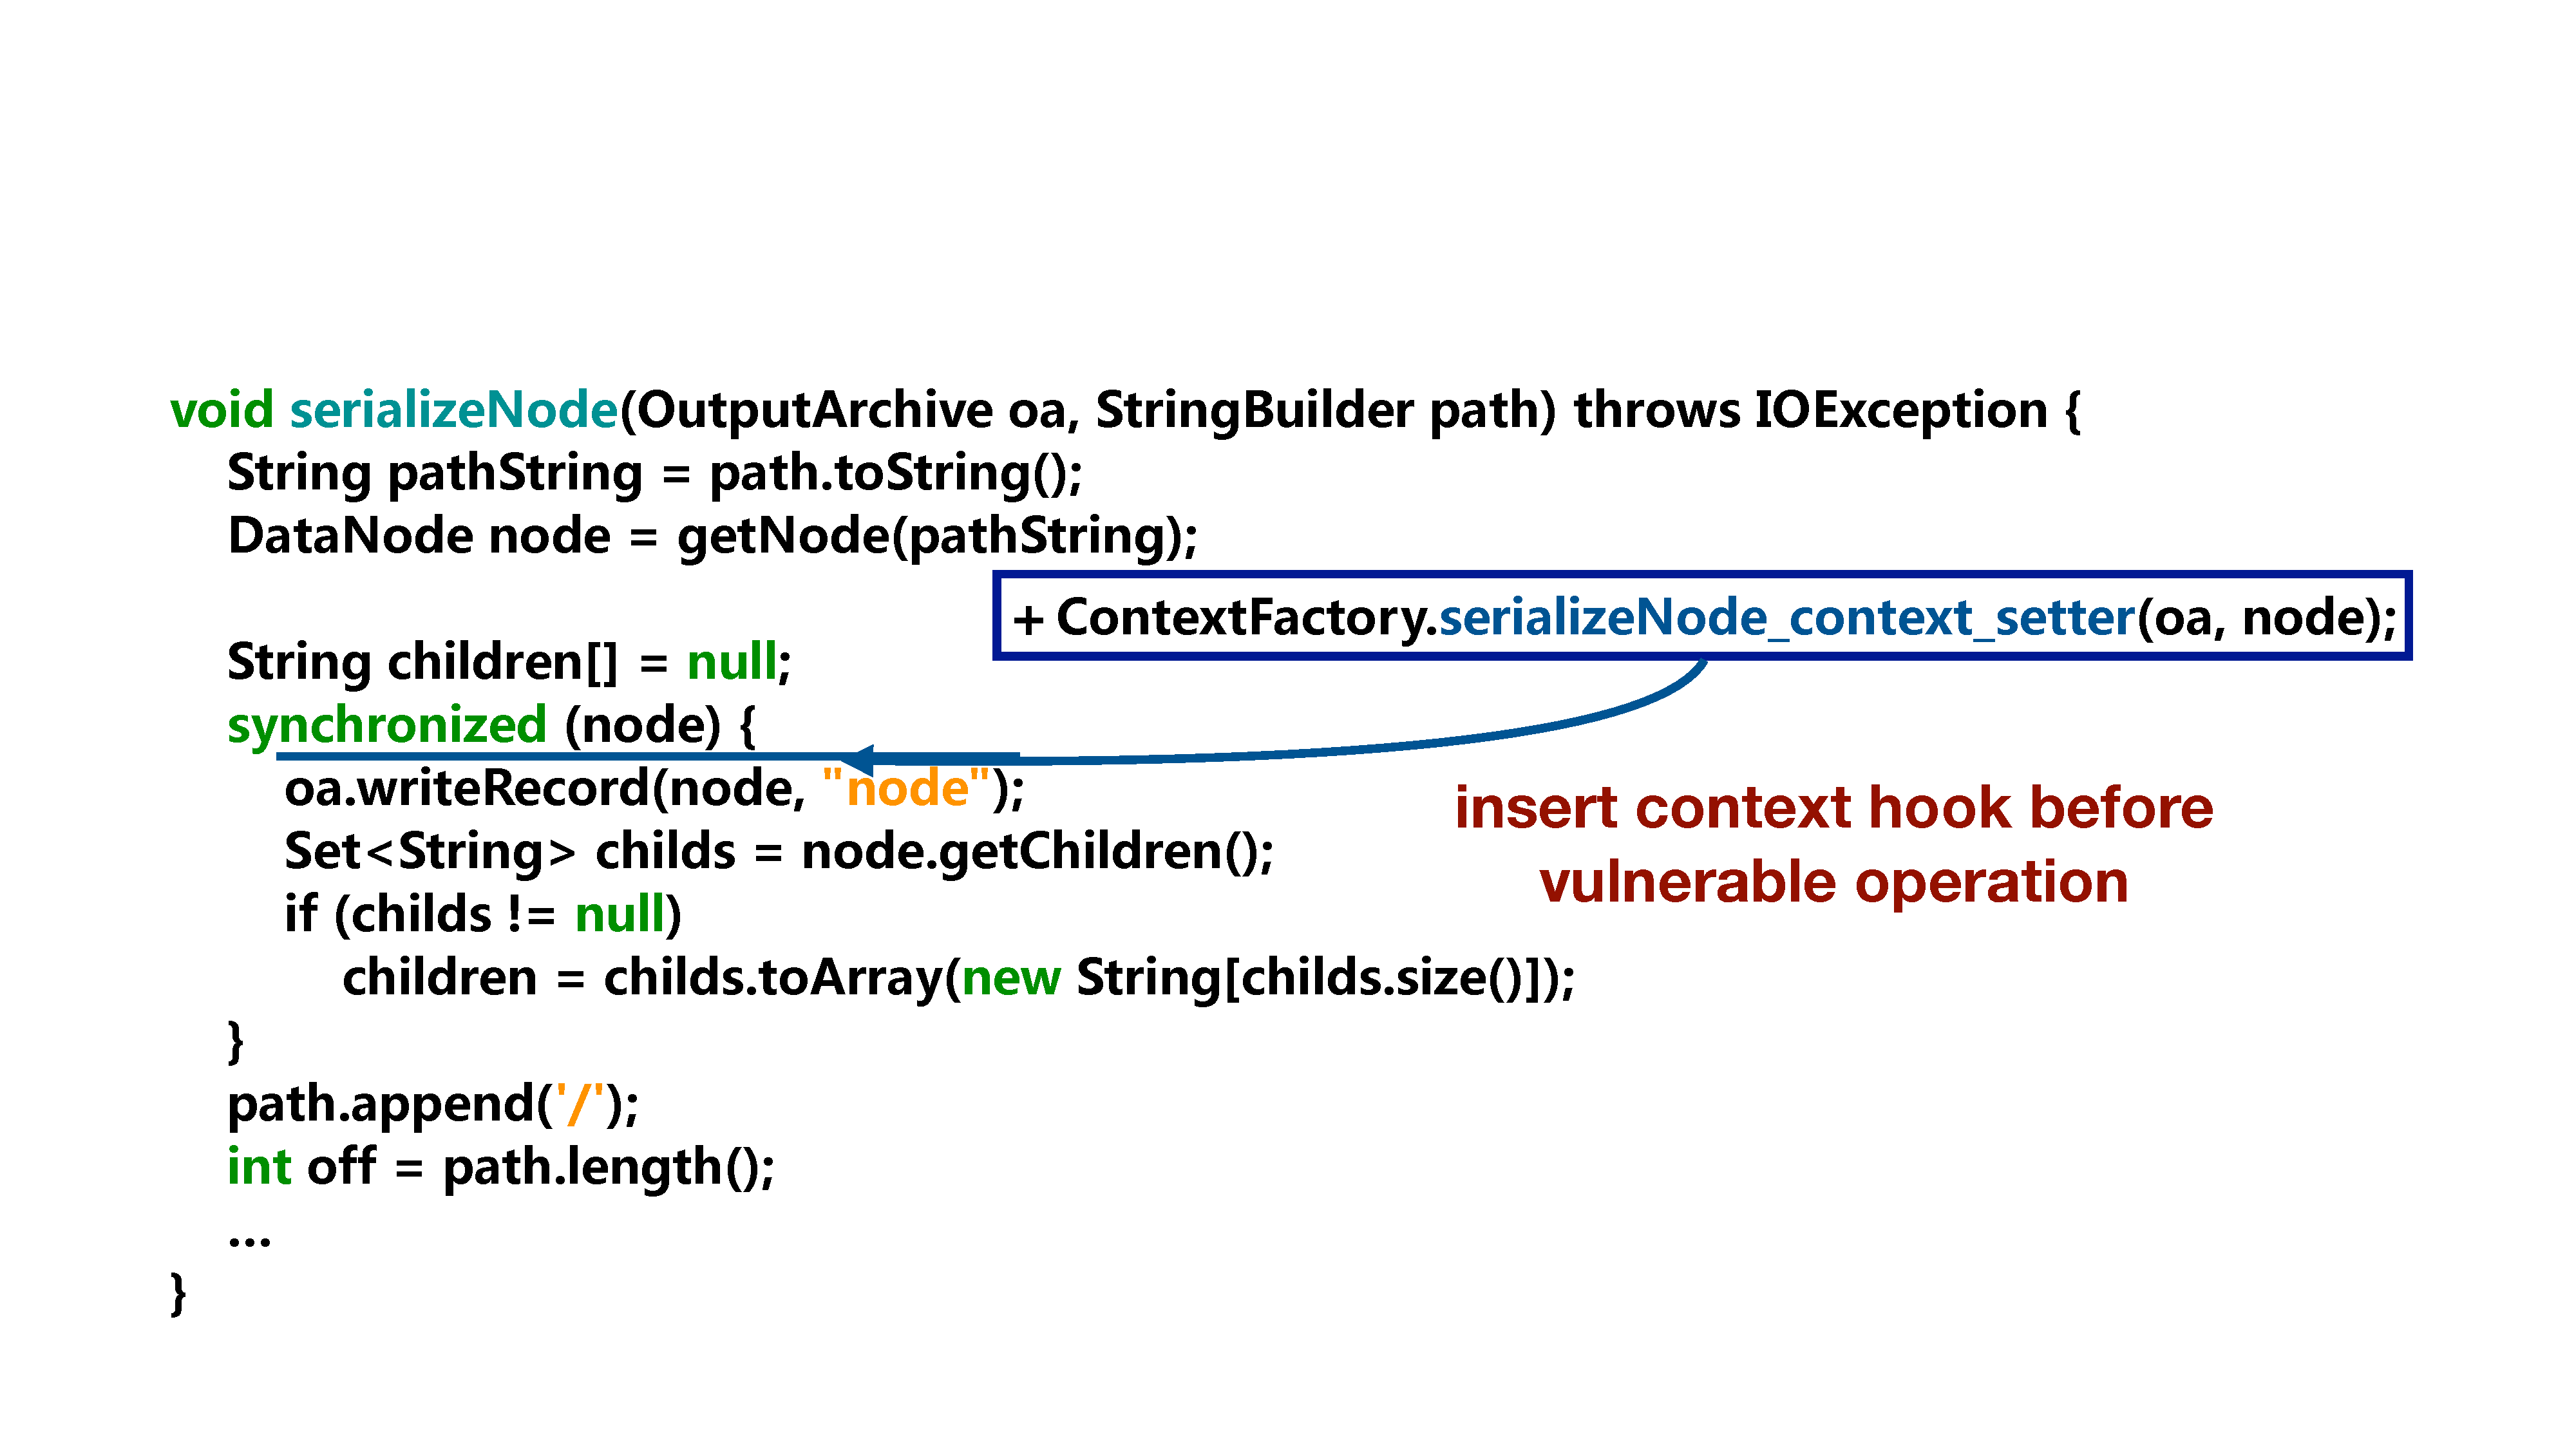
\includegraphics[width=.95\textwidth]{fig/hook}
    \end{center}
\end{frame}

\begin{frame}{An overview example}
    \begin{center}
        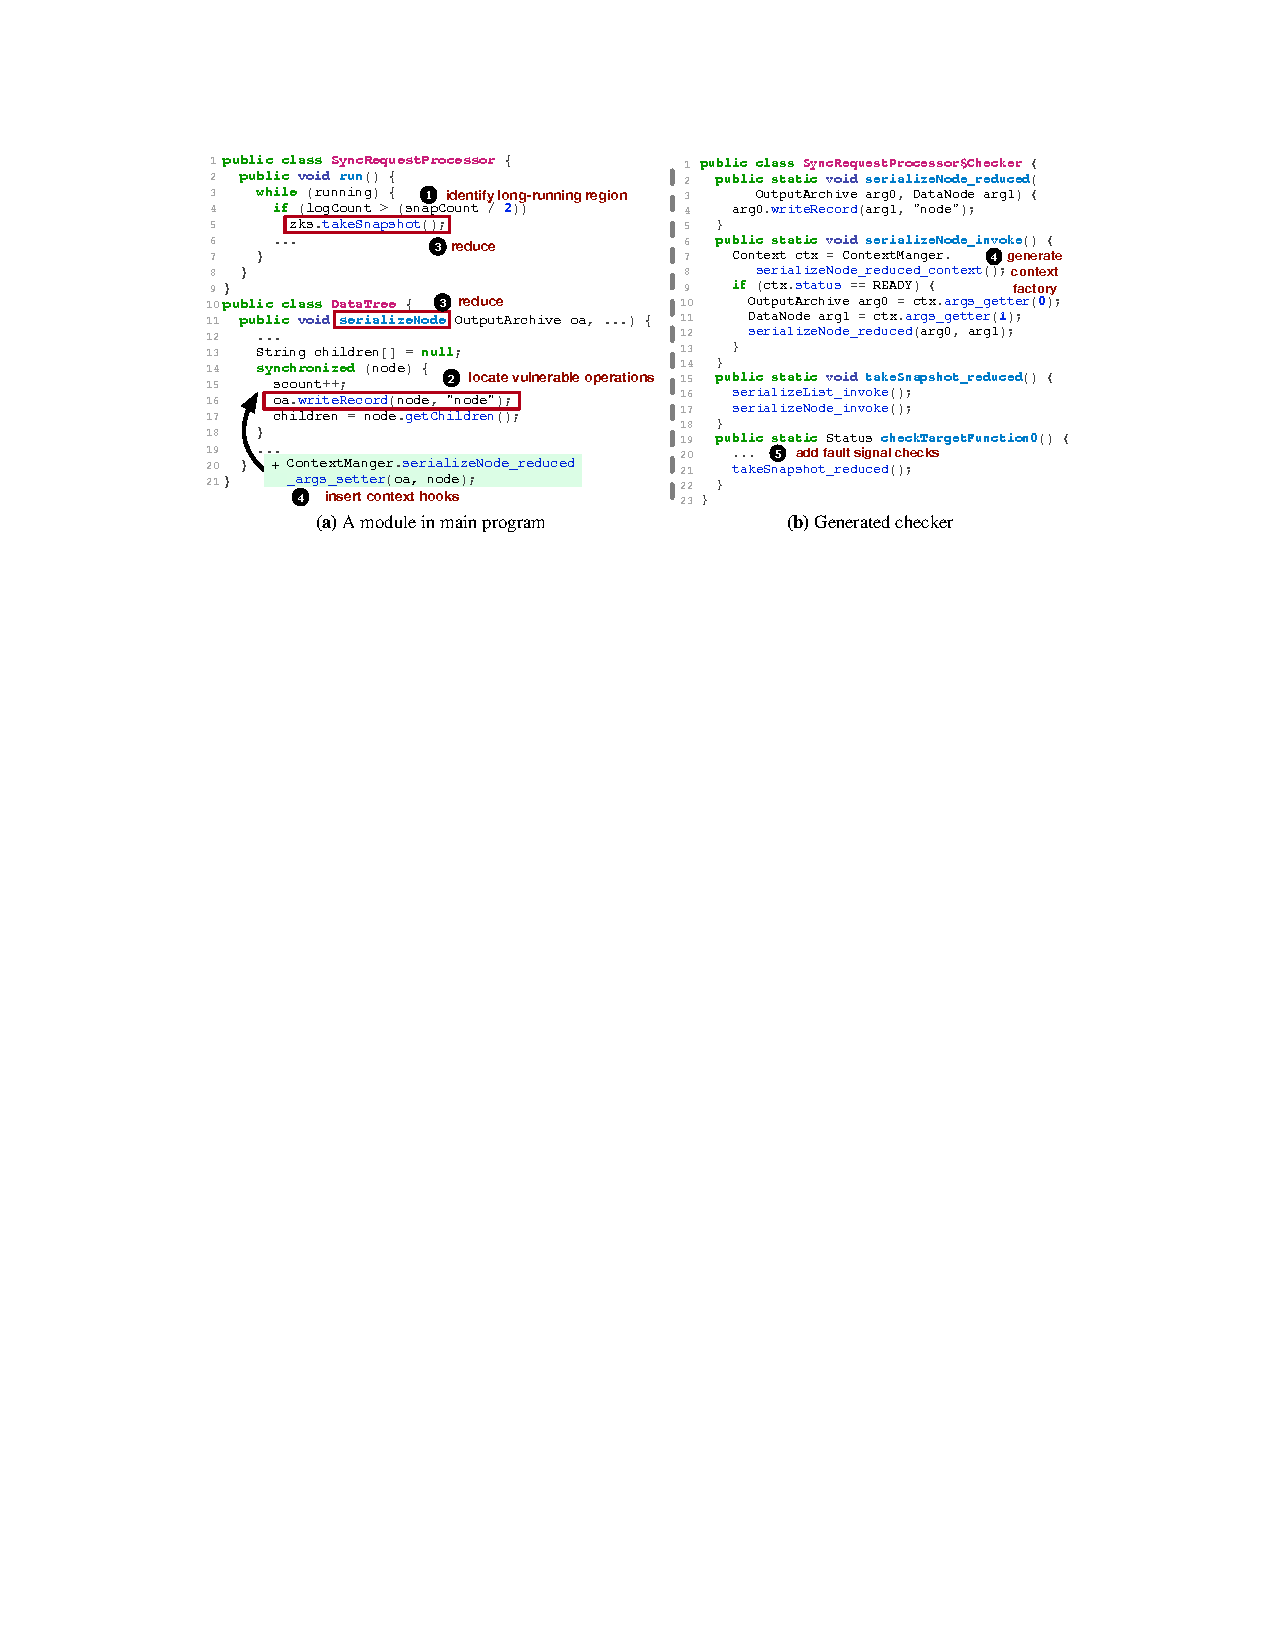
\includegraphics[width=\textwidth]{fig/compare}
    \end{center}
\end{frame}

\begin{frame}{Validate Impact of Caught Faults}
    \begin{block}{Transient or tolerable}
        \begin{itemize}
            \item e.g. transient network delay that caused no damage
        \end{itemize}
    \end{block}

    \begin{block}{Default: simply re-executes the checker and compare for transient errors}
        \begin{itemize}
            \item  allows developers write their own user-defined validation tasks to check some entry functions, e.g., \texttt{processRequest(req)}
            \item automate the part of deciding which validation task to invoke depending on which checker failed
        \end{itemize}
    \end{block}

\end{frame}

\begin{frame}{Prevent Side Effects}
    \framesubtitle{Context Replication (memory isolation)}
    Context manager will replicate the checker context so that any modifications are contained in the watchdog’s state

    \begin{center}
        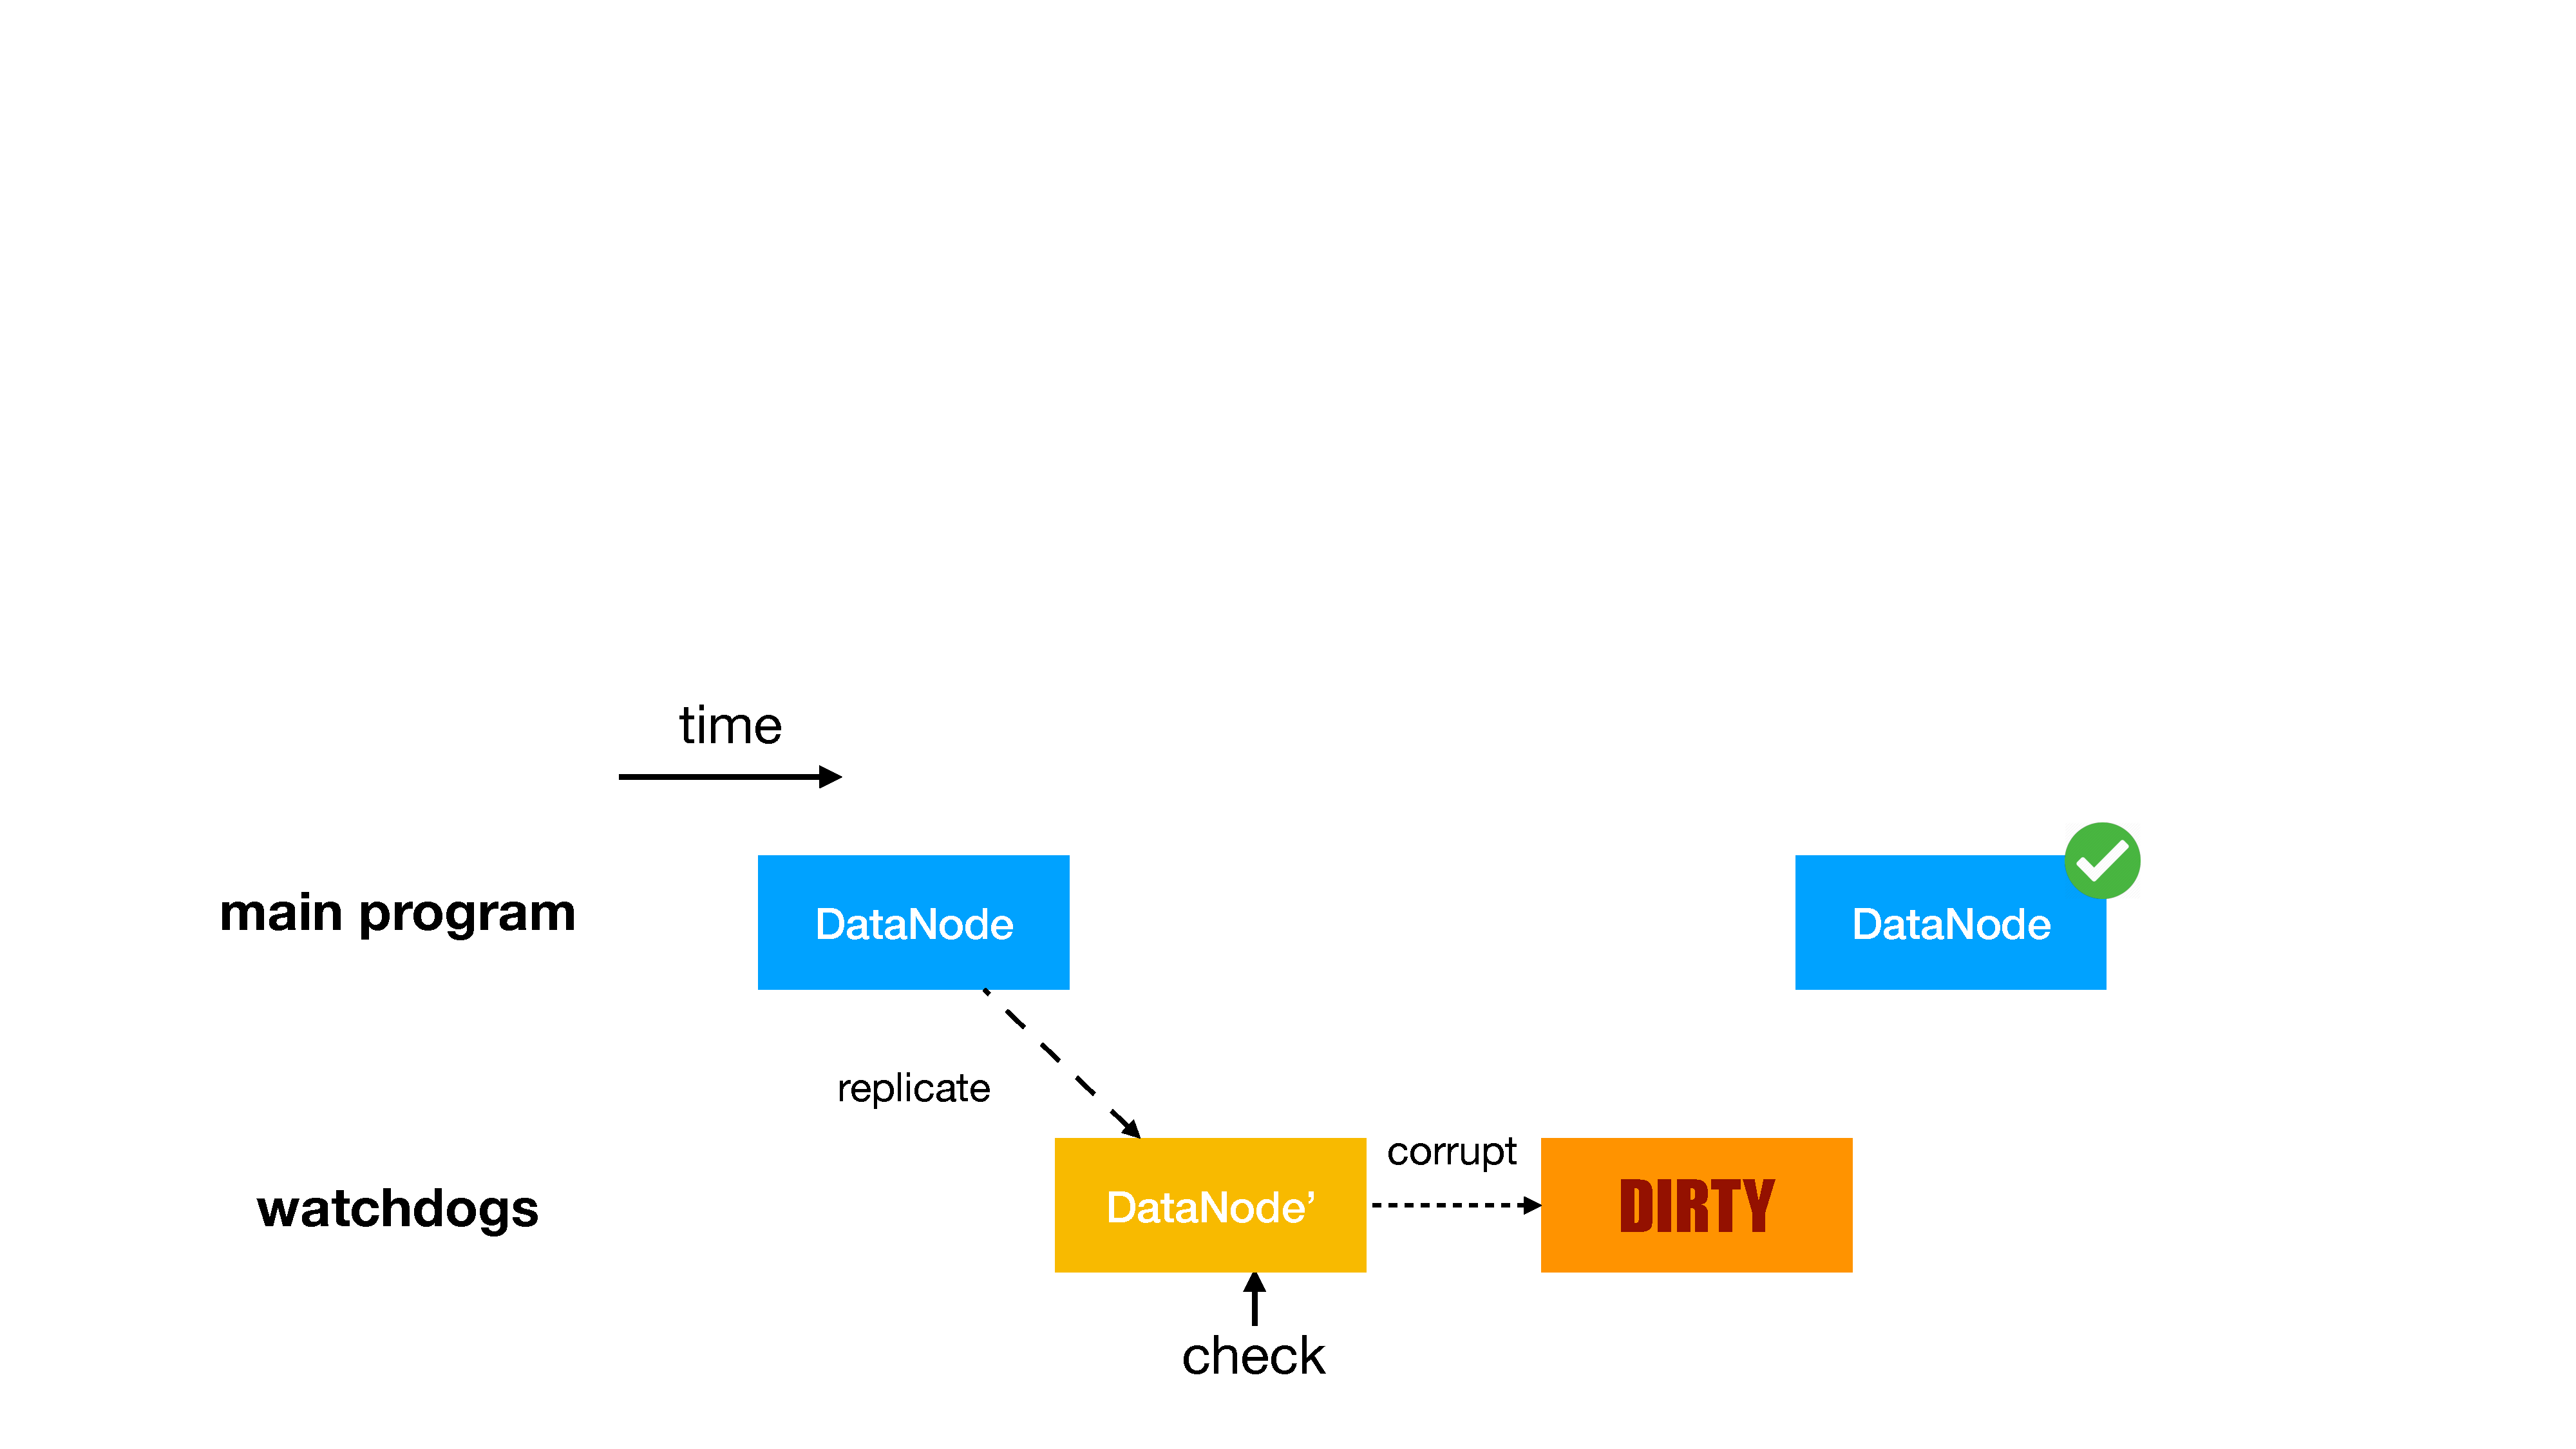
\includegraphics[width=.9\textwidth]{fig/replicate}
    \end{center}
\end{frame}

\begin{frame}{Prevent Side Effects}
    \framesubtitle{Context Replication (memory isolation)}
    To reduce performance overhead: immutability analysis + lazy copy
    \begin{center}
        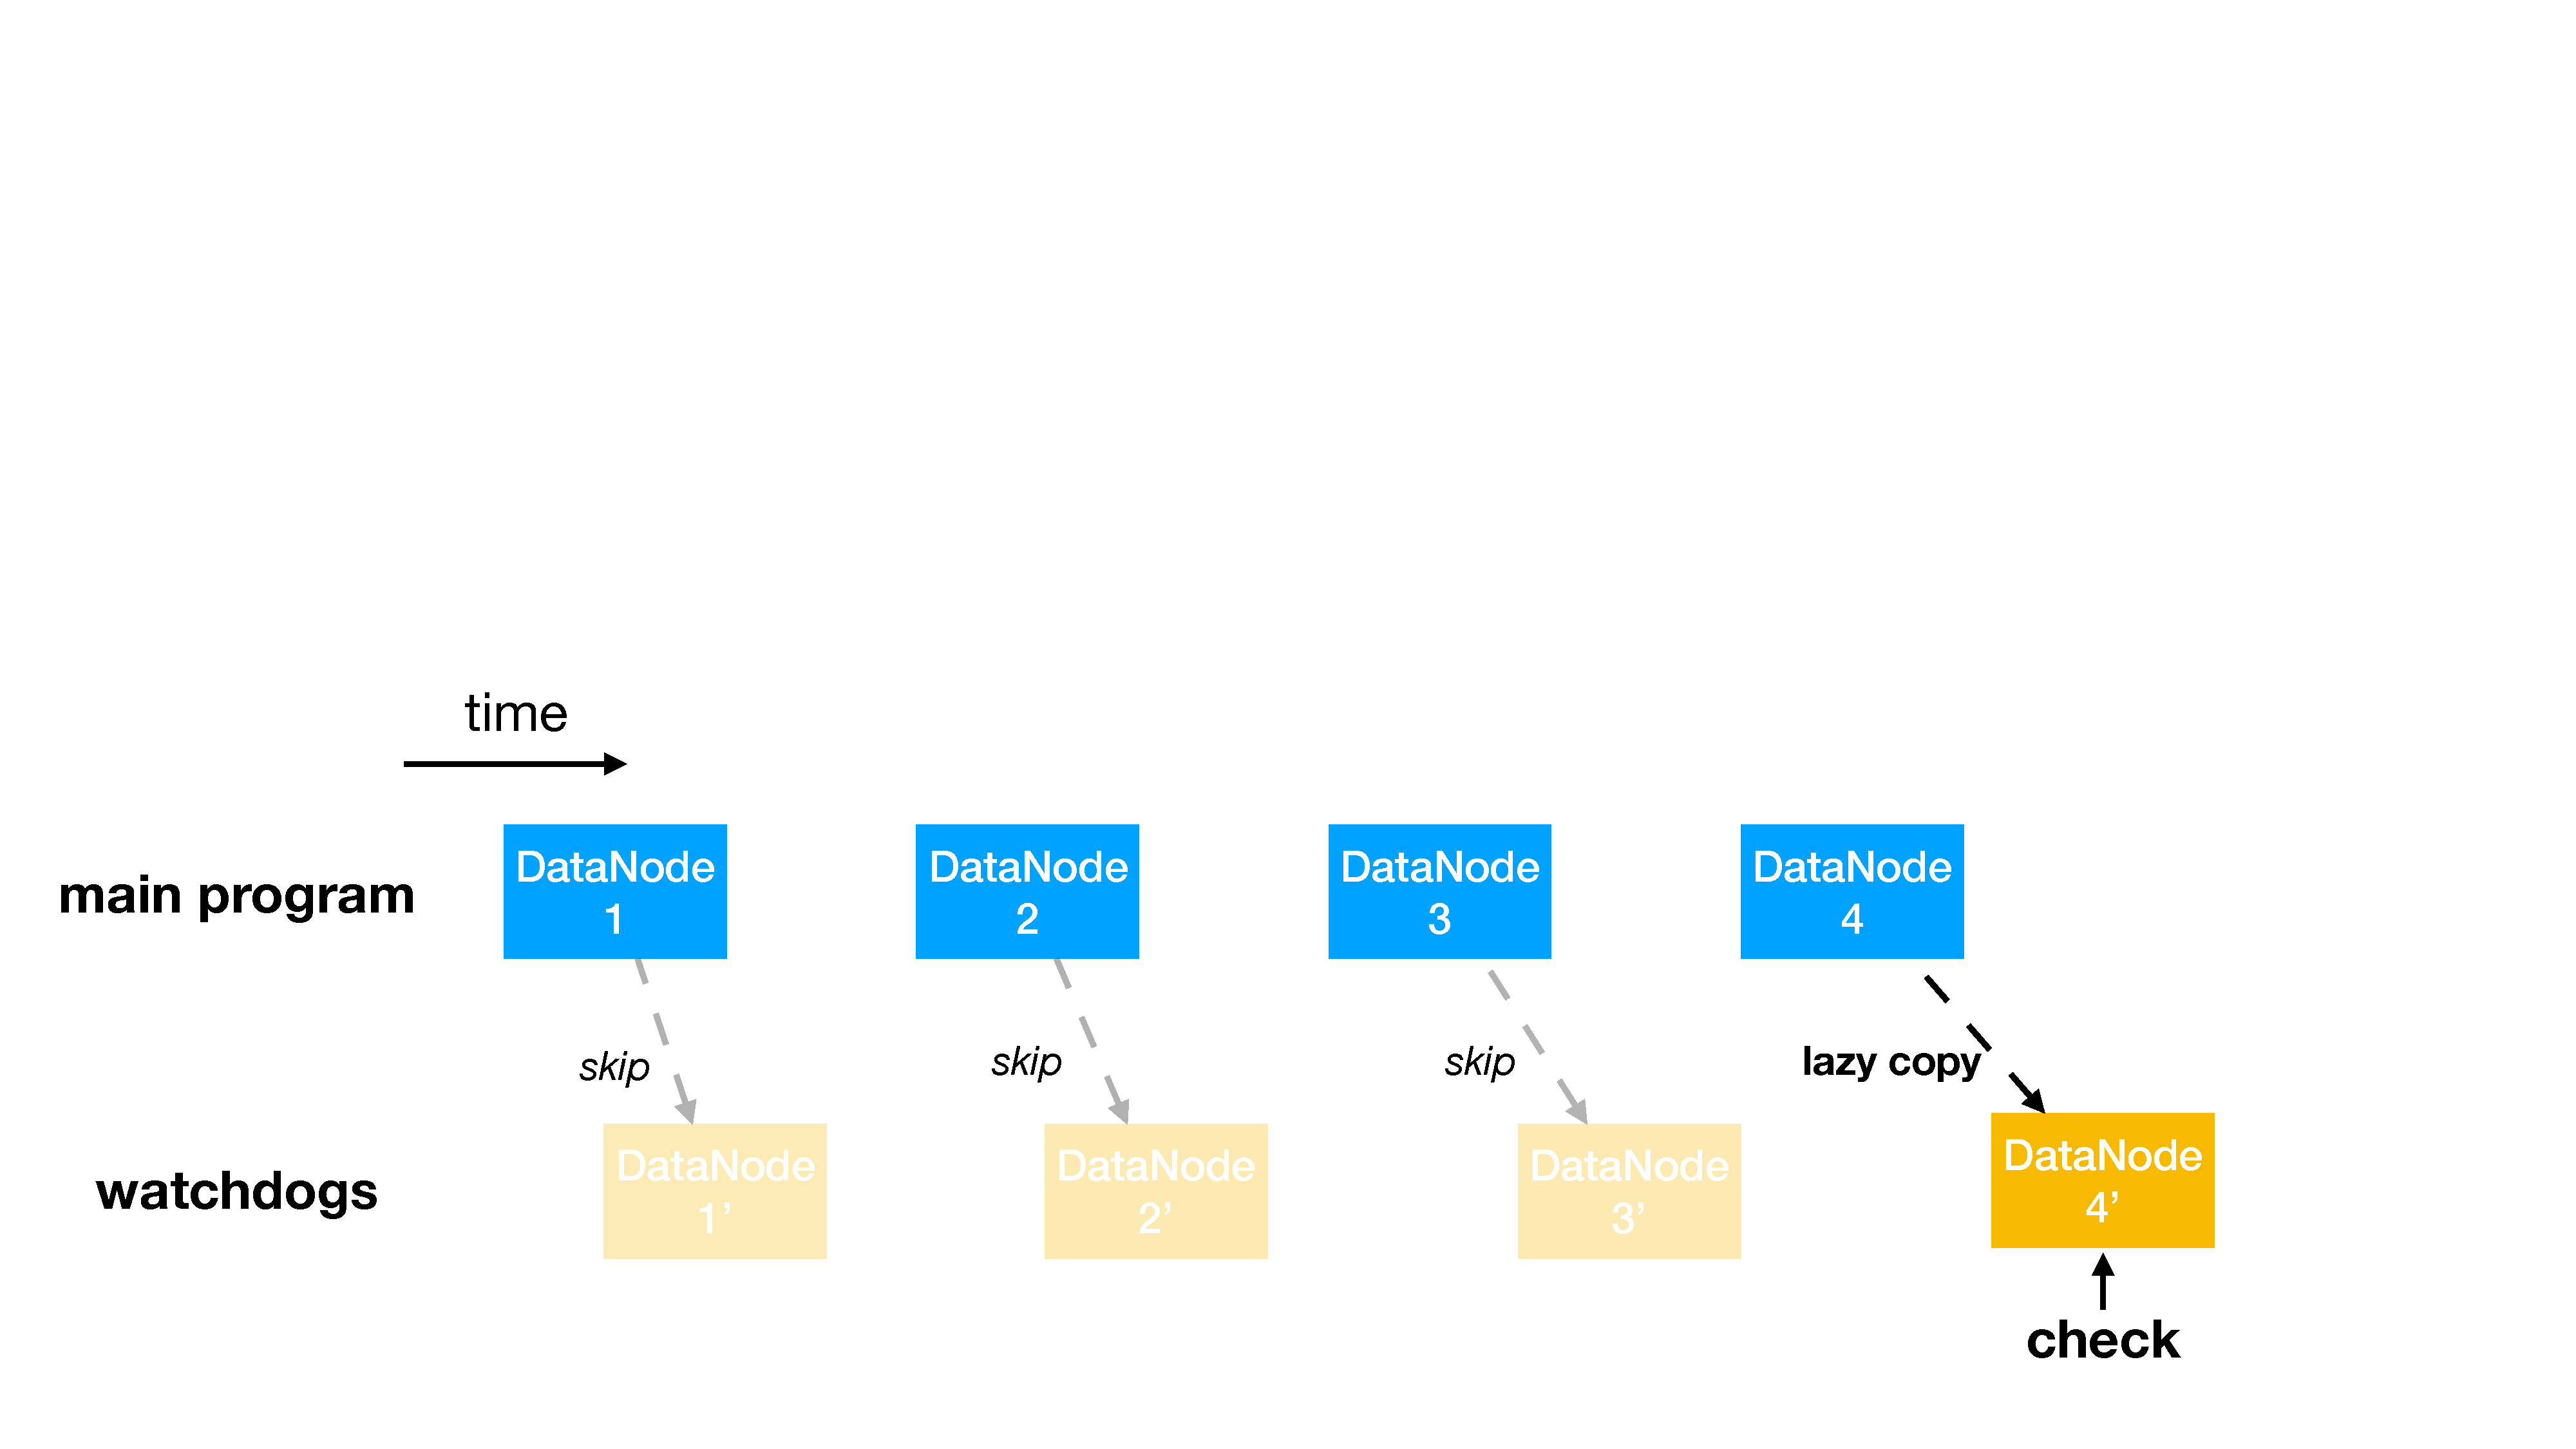
\includegraphics[width=.9\textwidth]{fig/lazy-copy}
    \end{center}
\end{frame}

\begin{frame}{Prevent Side Effects}
    \framesubtitle{Context Replication (memory isolation)}
    \begin{block}{Check consistency before copying and invocation with hashCode and versioning}
        Context attributes: \texttt{version}, \texttt{weak\_ref} and \texttt{hash}
        \begin{itemize}
            \item The lazy setter only sets these attributes without replicate the context.
            \item If getter invoked, check \texttt{weak\_ref!=null}
            \item Check if hash code of the referent’s value matches \texttt{hash}
        \end{itemize}
    \end{block}
    \begin{center}
        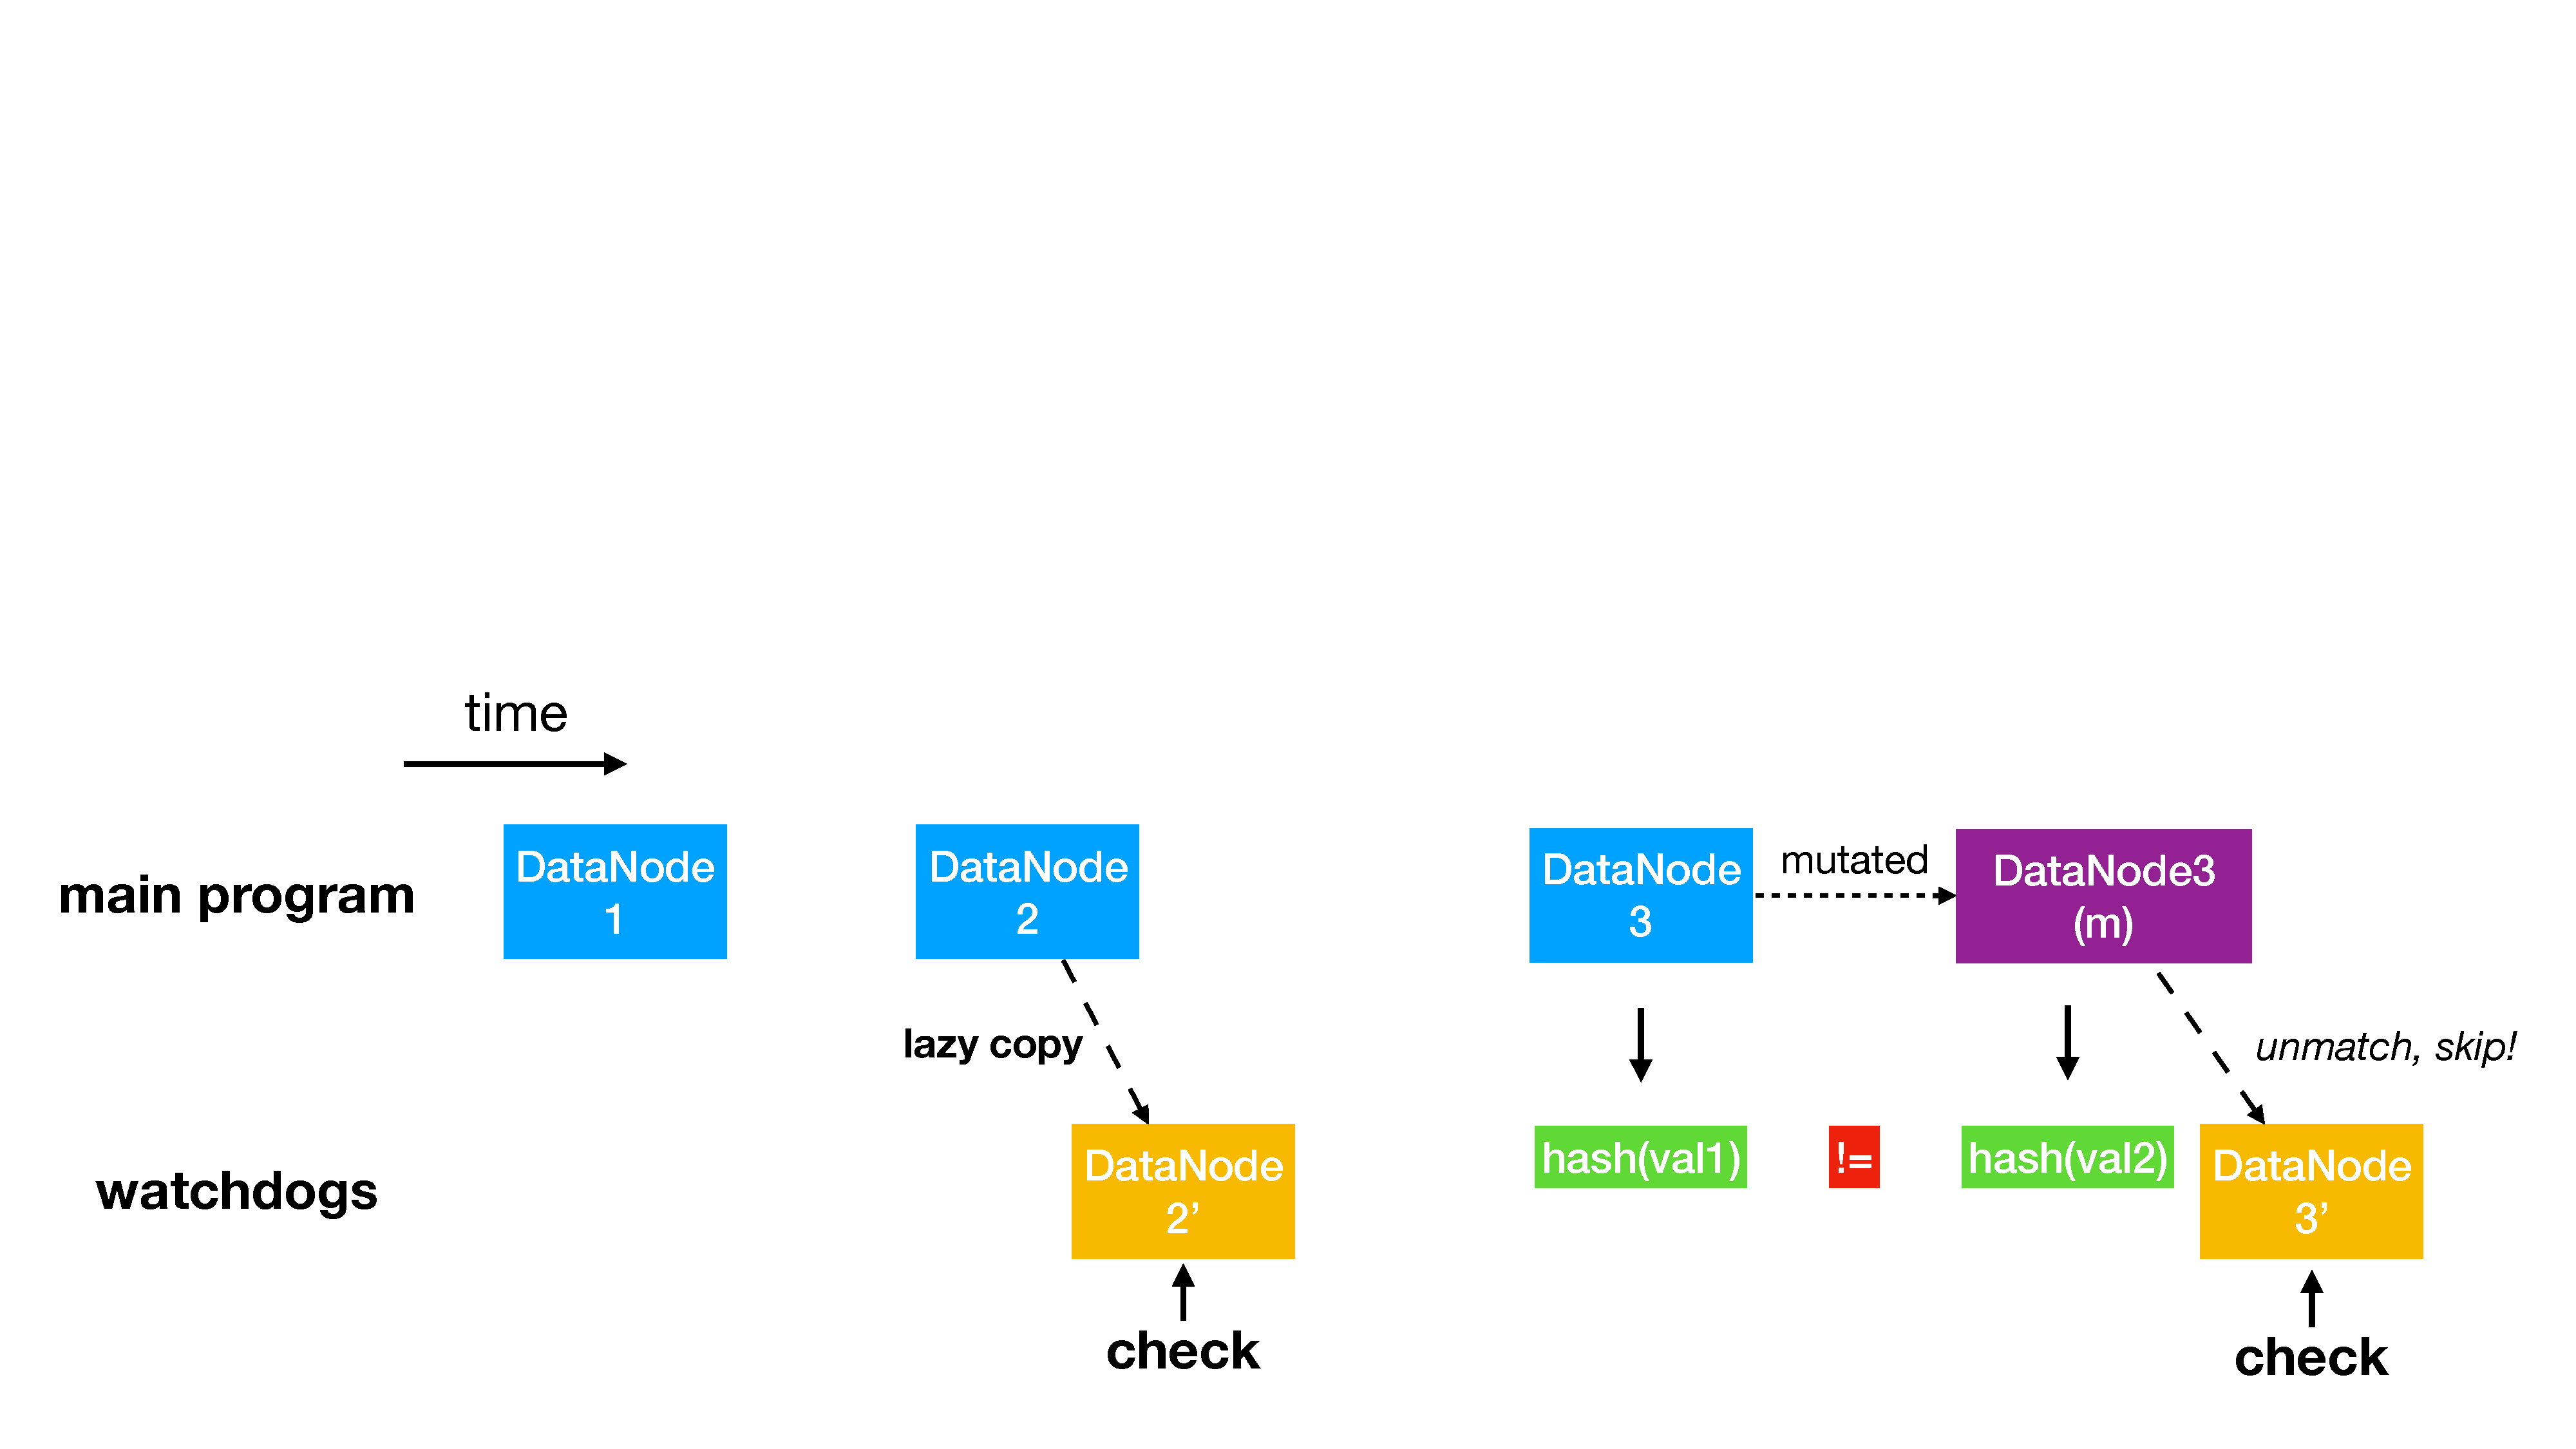
\includegraphics[width=.8\textwidth]{fig/hash}
    \end{center}
\end{frame}

\begin{frame}{Prevent Side Effects}
    \framesubtitle{I/O Redirection and Idempotent Wrappers (I/O isolation)}
    \begin{description}
        \item[\textbf{write:}] file-related resource replicated with target path changed to test file
        \item[\textbf{read:}] let watchdogs pre-read contexts and cache
    \end{description}

    \begin{center}
        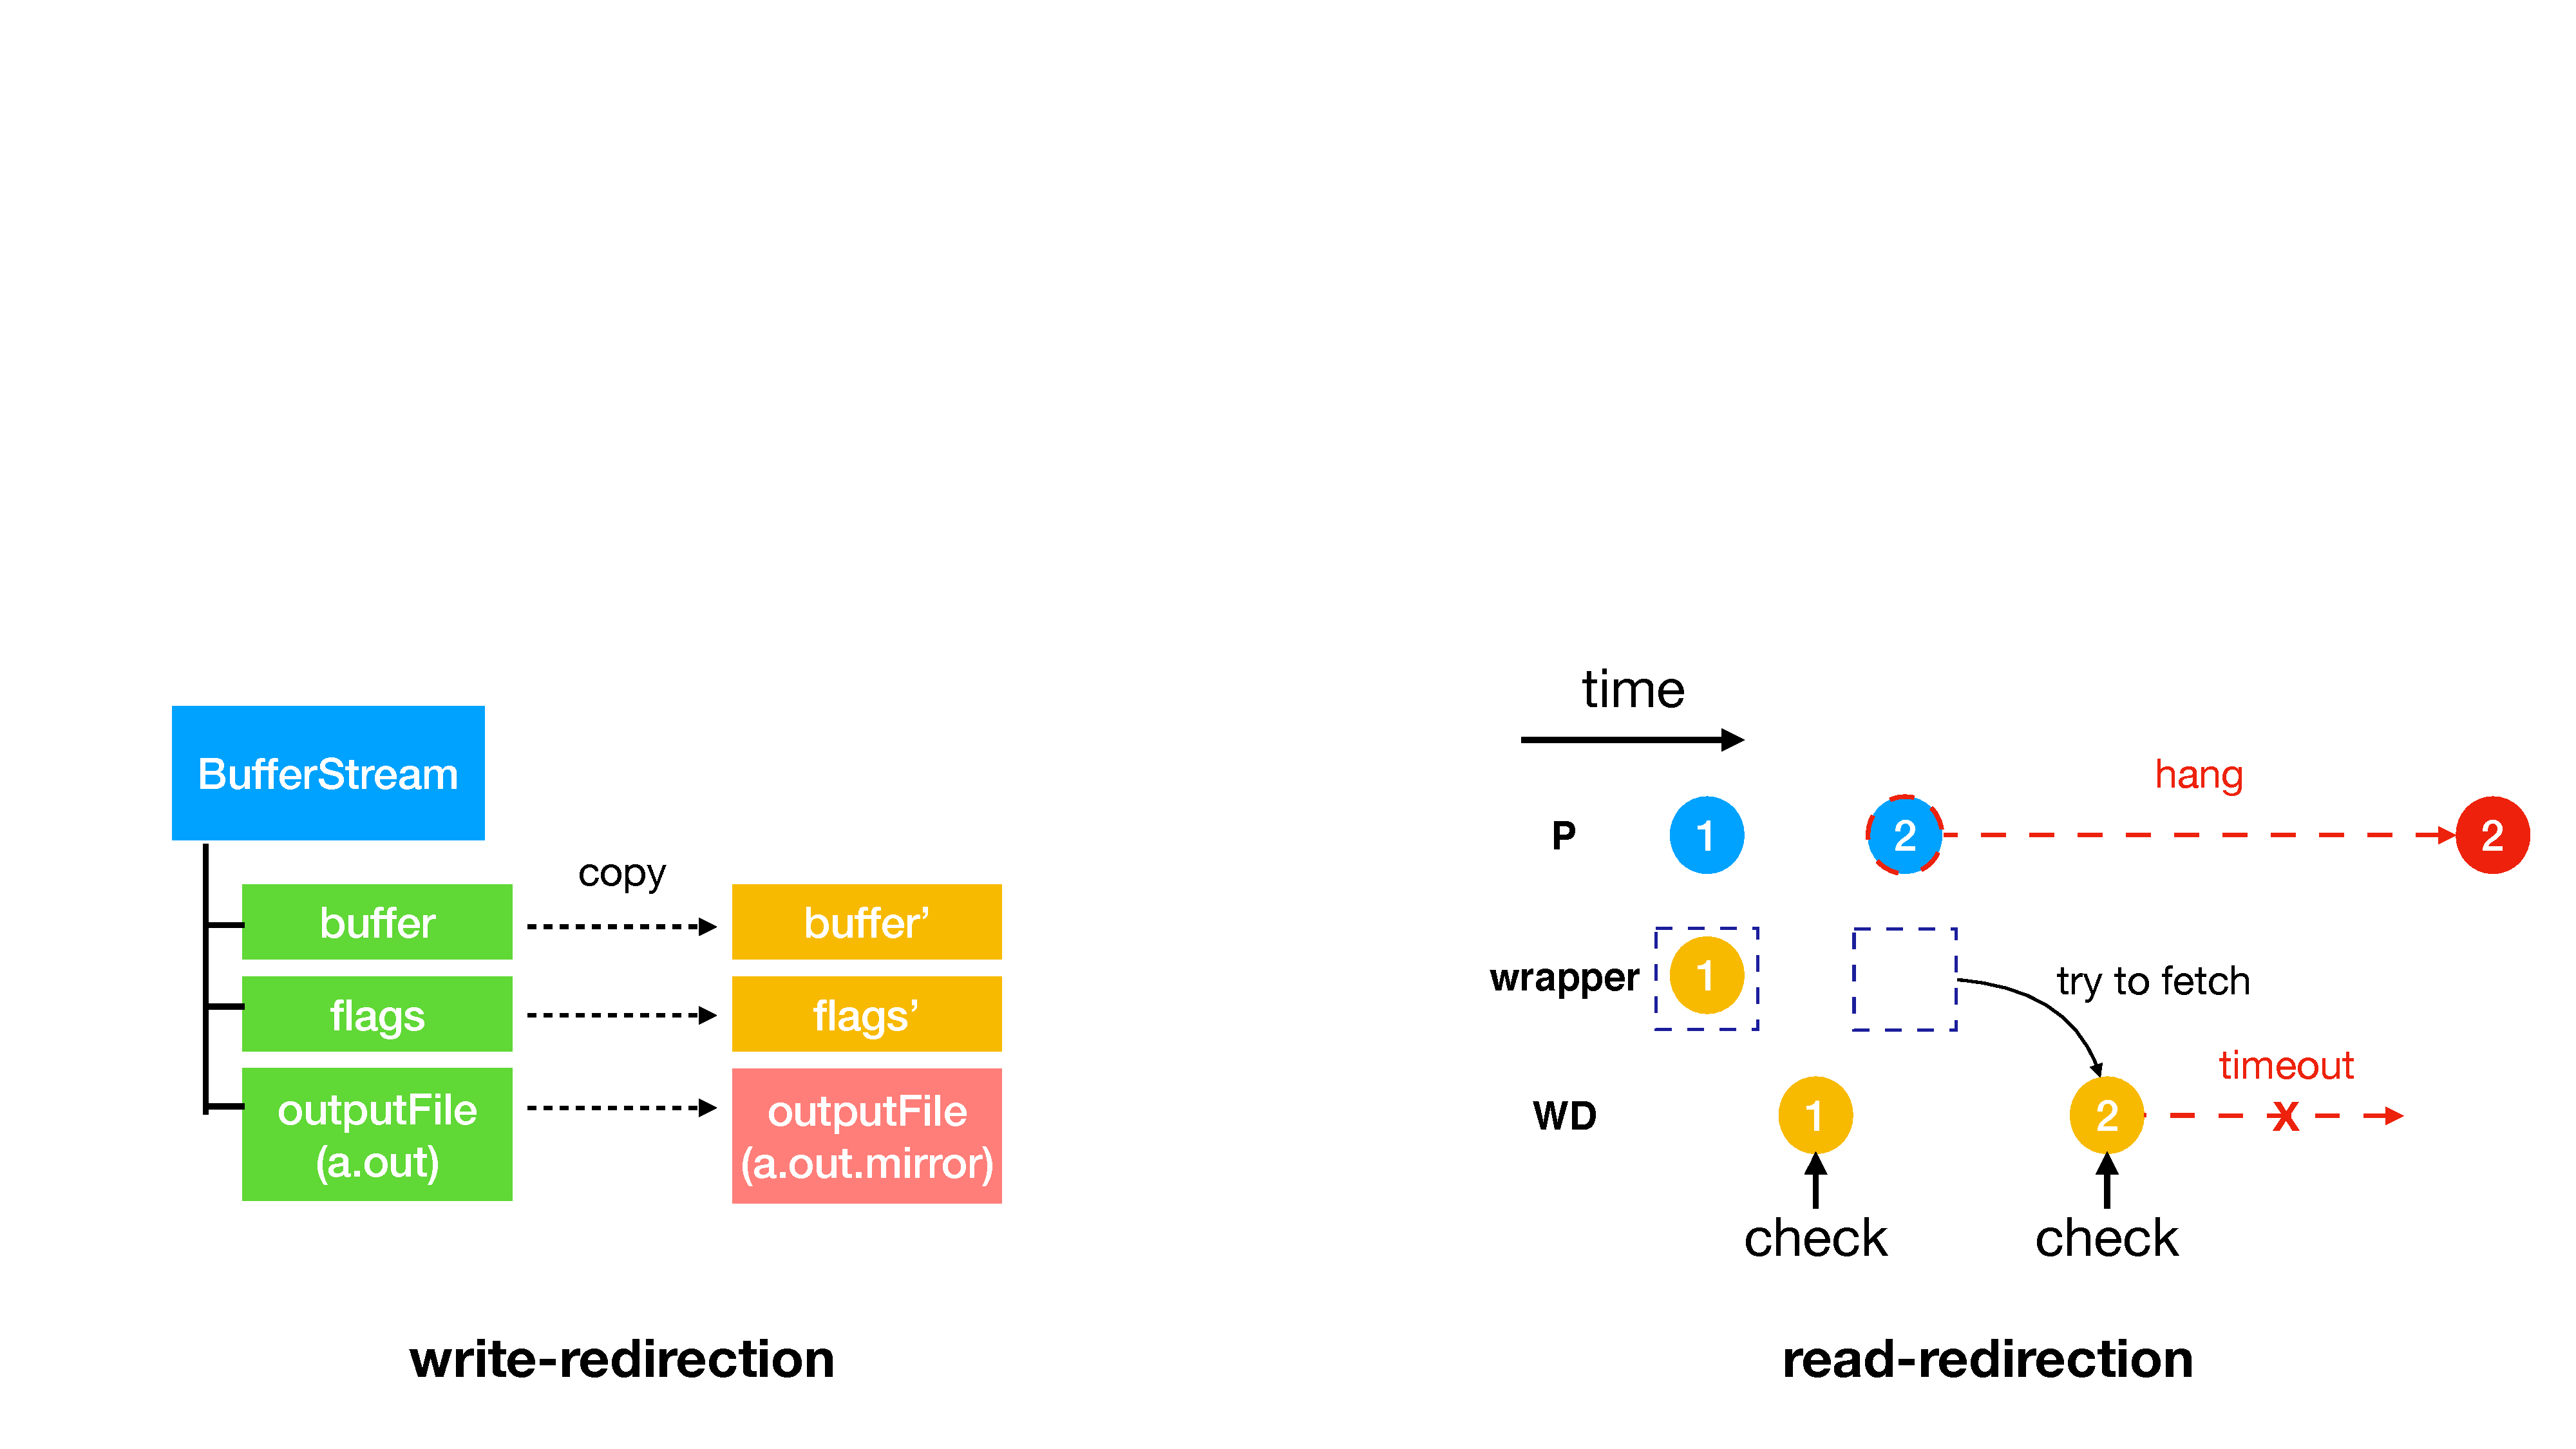
\includegraphics[width=.9\textwidth]{fig/io}
    \end{center}
\end{frame}
\section{Evaluation}
\begin{frame}{Experiments}
    \framesubtitle{Scale \& Generated watchdog}
    \begin{tabular}{c|c|c|c|c|c|c}
        \toprule
                   & ZooKeeper & Cassandra & HDFS   & HBase   & MapReduce & Yarn   \\
        \midrule
        SLOC       & 28K       & 102K      & 219K   & 728K    & 191K      & 229K   \\
        Methods    & 3,562     & 12,919    & 79,584 & 179,821 & 16,633    & 10,432 \\
        \midrule
        Watchdogs  & 96        & 190       & 174    & 358     & 161       & 88     \\
        Methods    & 118       & 464       & 482    & 795     & 371       & 222    \\
        Operations & 488       & 2,112     & 3,416  & 9,557   & 6,116     & 752    \\
        \bottomrule
    \end{tabular}
\end{frame}

\begin{frame}[allowframebreaks]{22 Real-world Partial Failures Reproduced for Evaluation}
    \begin{longtable}{c|c|c|c|c|c}
        \toprule
        JIRA Id.       & Id. & Root Cause            & Conseq.   & Sticky? & Study? \\
        \midrule
        ZooKeeper-2201 & ZK1 & Bad Synch.            & Stuck     & No      & Yes    \\
        ZooKeeper-602  & ZK2 & Uncaught Error        & Zombie    & Yes     & Yes    \\
        ZooKeeper-2325 & ZK3 & Logic Error           & Inconsist & Yes     & No     \\
        ZooKeeper-3131 & ZK4 & Resource  Leak        & Slow      & Yes     & Yes    \\
        \midrule
        Cassandra-6364 & CS1 & Uncaught  Error       & Zombie    & Yes     & Yes    \\
        Cassandra-6415 & CS2 & Indefinite Blocking   & Stuck     & No      & Yes    \\
        Cassandra-9549 & CS3 & Resource Leak         & Slow      & Yes     & No     \\
        Cassandra-9486 & CS4 & Performance   Bug     & Slow      & Yes     & No     \\
        \midrule
        HDFS-8429      & HF1 & Uncaught Error        & Stuck     & Yes     & Yes    \\
        HDFS-11377     & HF2 & Indefinite Blocking   & Stuck     & No      & Yes    \\
        HDFS-11352     & HF3 & Deadlock              & Stuck     & Yes     & No     \\
        HDFS-4233      & HF4 & Uncaught  Error       & Data Loss & Yes     & No     \\
        \midrule
        HBase-18137    & HB1 & Infinite Loop         & Stuck     & Yes     & No     \\
        HBase-16429    & HB2 & Deadlock              & Stuck     & Yes     & No     \\
        HBase-21464    & HB3 & Logic Error           & Stuck     & Yes     & No     \\
        HBase-21357    & HB4 & Uncaught Error        & Denial    & Yes     & No     \\
        HBase-16081    & HB5 & Indefinite Blocking   & Silent    & Yes     & No     \\
        \midrule
        MapReduce-6351 & MR1 & Deadlock              & Stuck     & Yes     & No     \\
        MapReduce-6190 & MR2 & Infinite Loop         & Stuck     & Yes     & No     \\
        MapReduce-6957 & MR3 & Improper Err Handling & Stuck     & Yes     & No     \\
        MapReduce-3634 & MR4 & Uncaught Error        & Zombie    & Yes     & No     \\
        \midrule
        Yarn-4254      & YN1 & Improper Err Handling & Stuck     & Yes     & No     \\
        \bottomrule
    \end{longtable}
\end{frame}

\begin{frame}{Baseline}
    \begin{description}
        \item[\textbf{Client}] \texttt{Panorama}\footfullcite{huang2018capturing}: instrument and monitor client responses
        \item[\textbf{Probe}]  \texttt{Falcon}\footfullcite{leners2011detecting}: daemon thread in the process that periodically invokes internal functions with synthetic requests
        \item[\textbf{Signal}] script that scans logs and checks JMX metrics
        \item[\textbf{Resource}]  daemon thread that monitors memory usage, disk and I/O health, and active thread count
    \end{description}
\end{frame}

\begin{frame}{Detection Time}
    \begin{itemize}
        \item median detection time: 4.2s
        \item 12 by default vulnerable operation rules
        \item 8  by system-specific rules
        \item effective for liveness issues like deadlock, indefinite blocking, and safe issues
        \item less effective for silent correctness errors
    \end{itemize}
    \begin{center}
        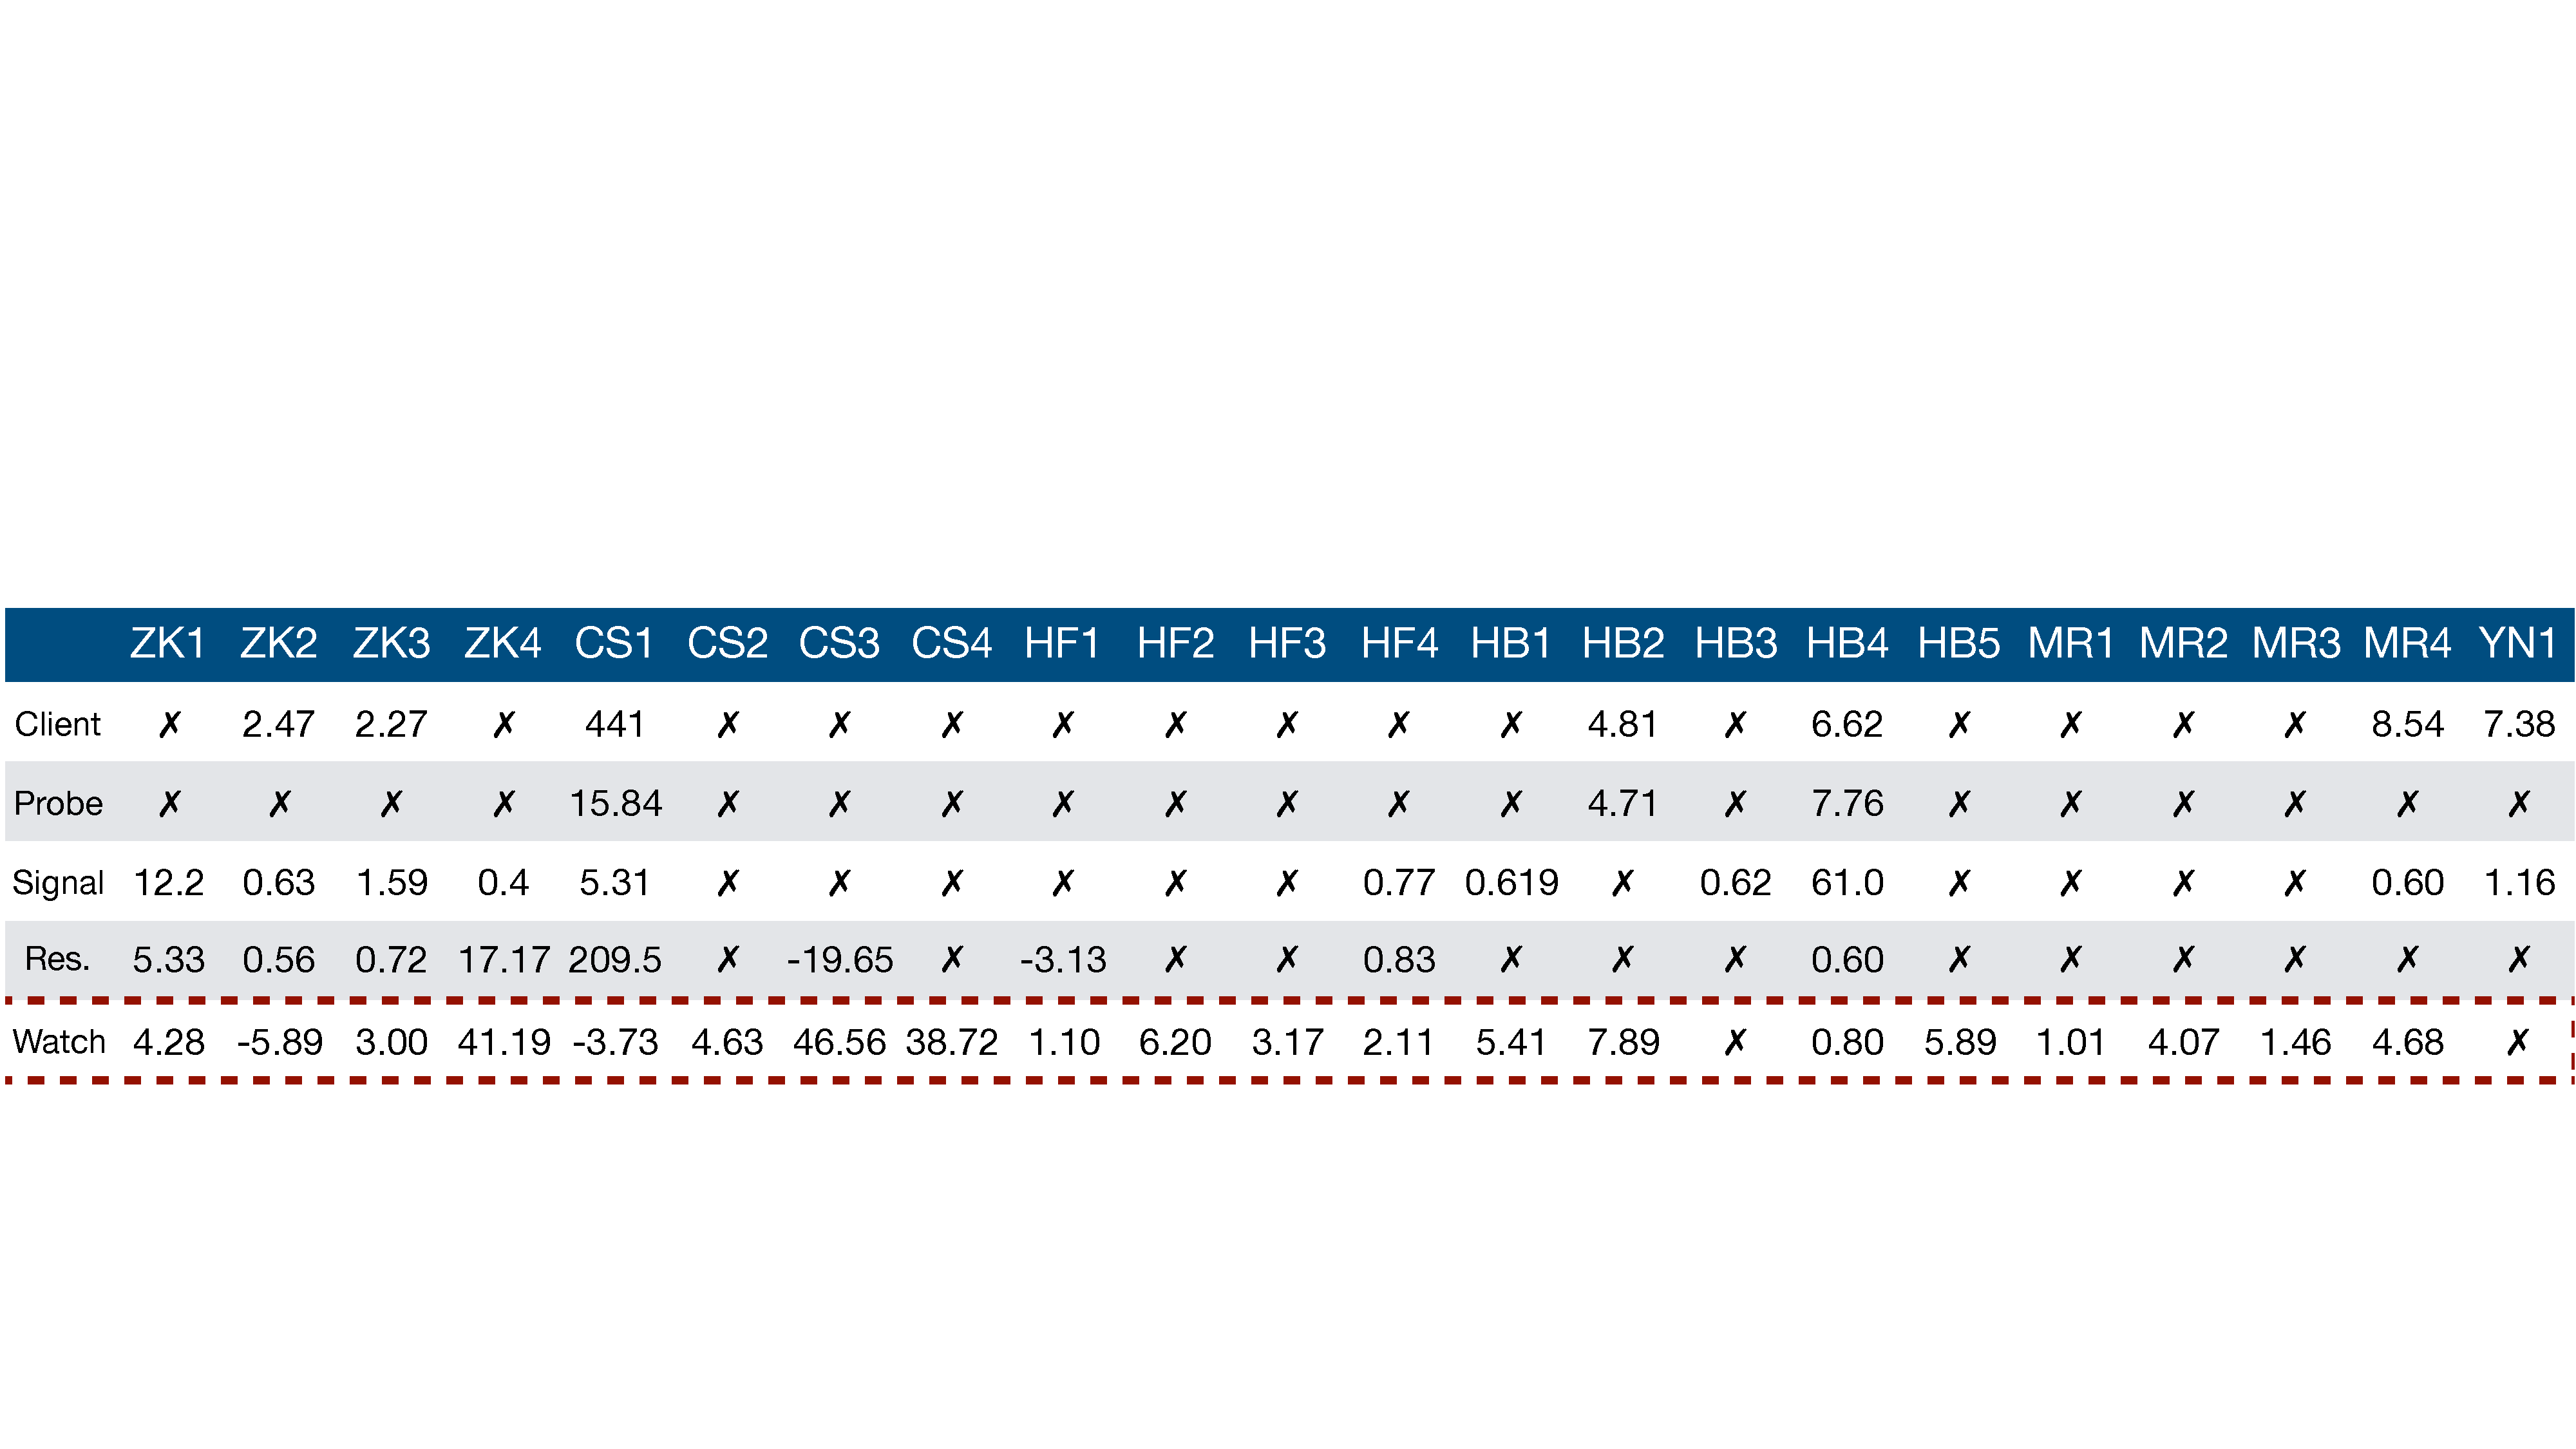
\includegraphics[width=1\textwidth]{fig/time}
    \end{center}
\end{frame}

\begin{frame}{Detection Localization}
    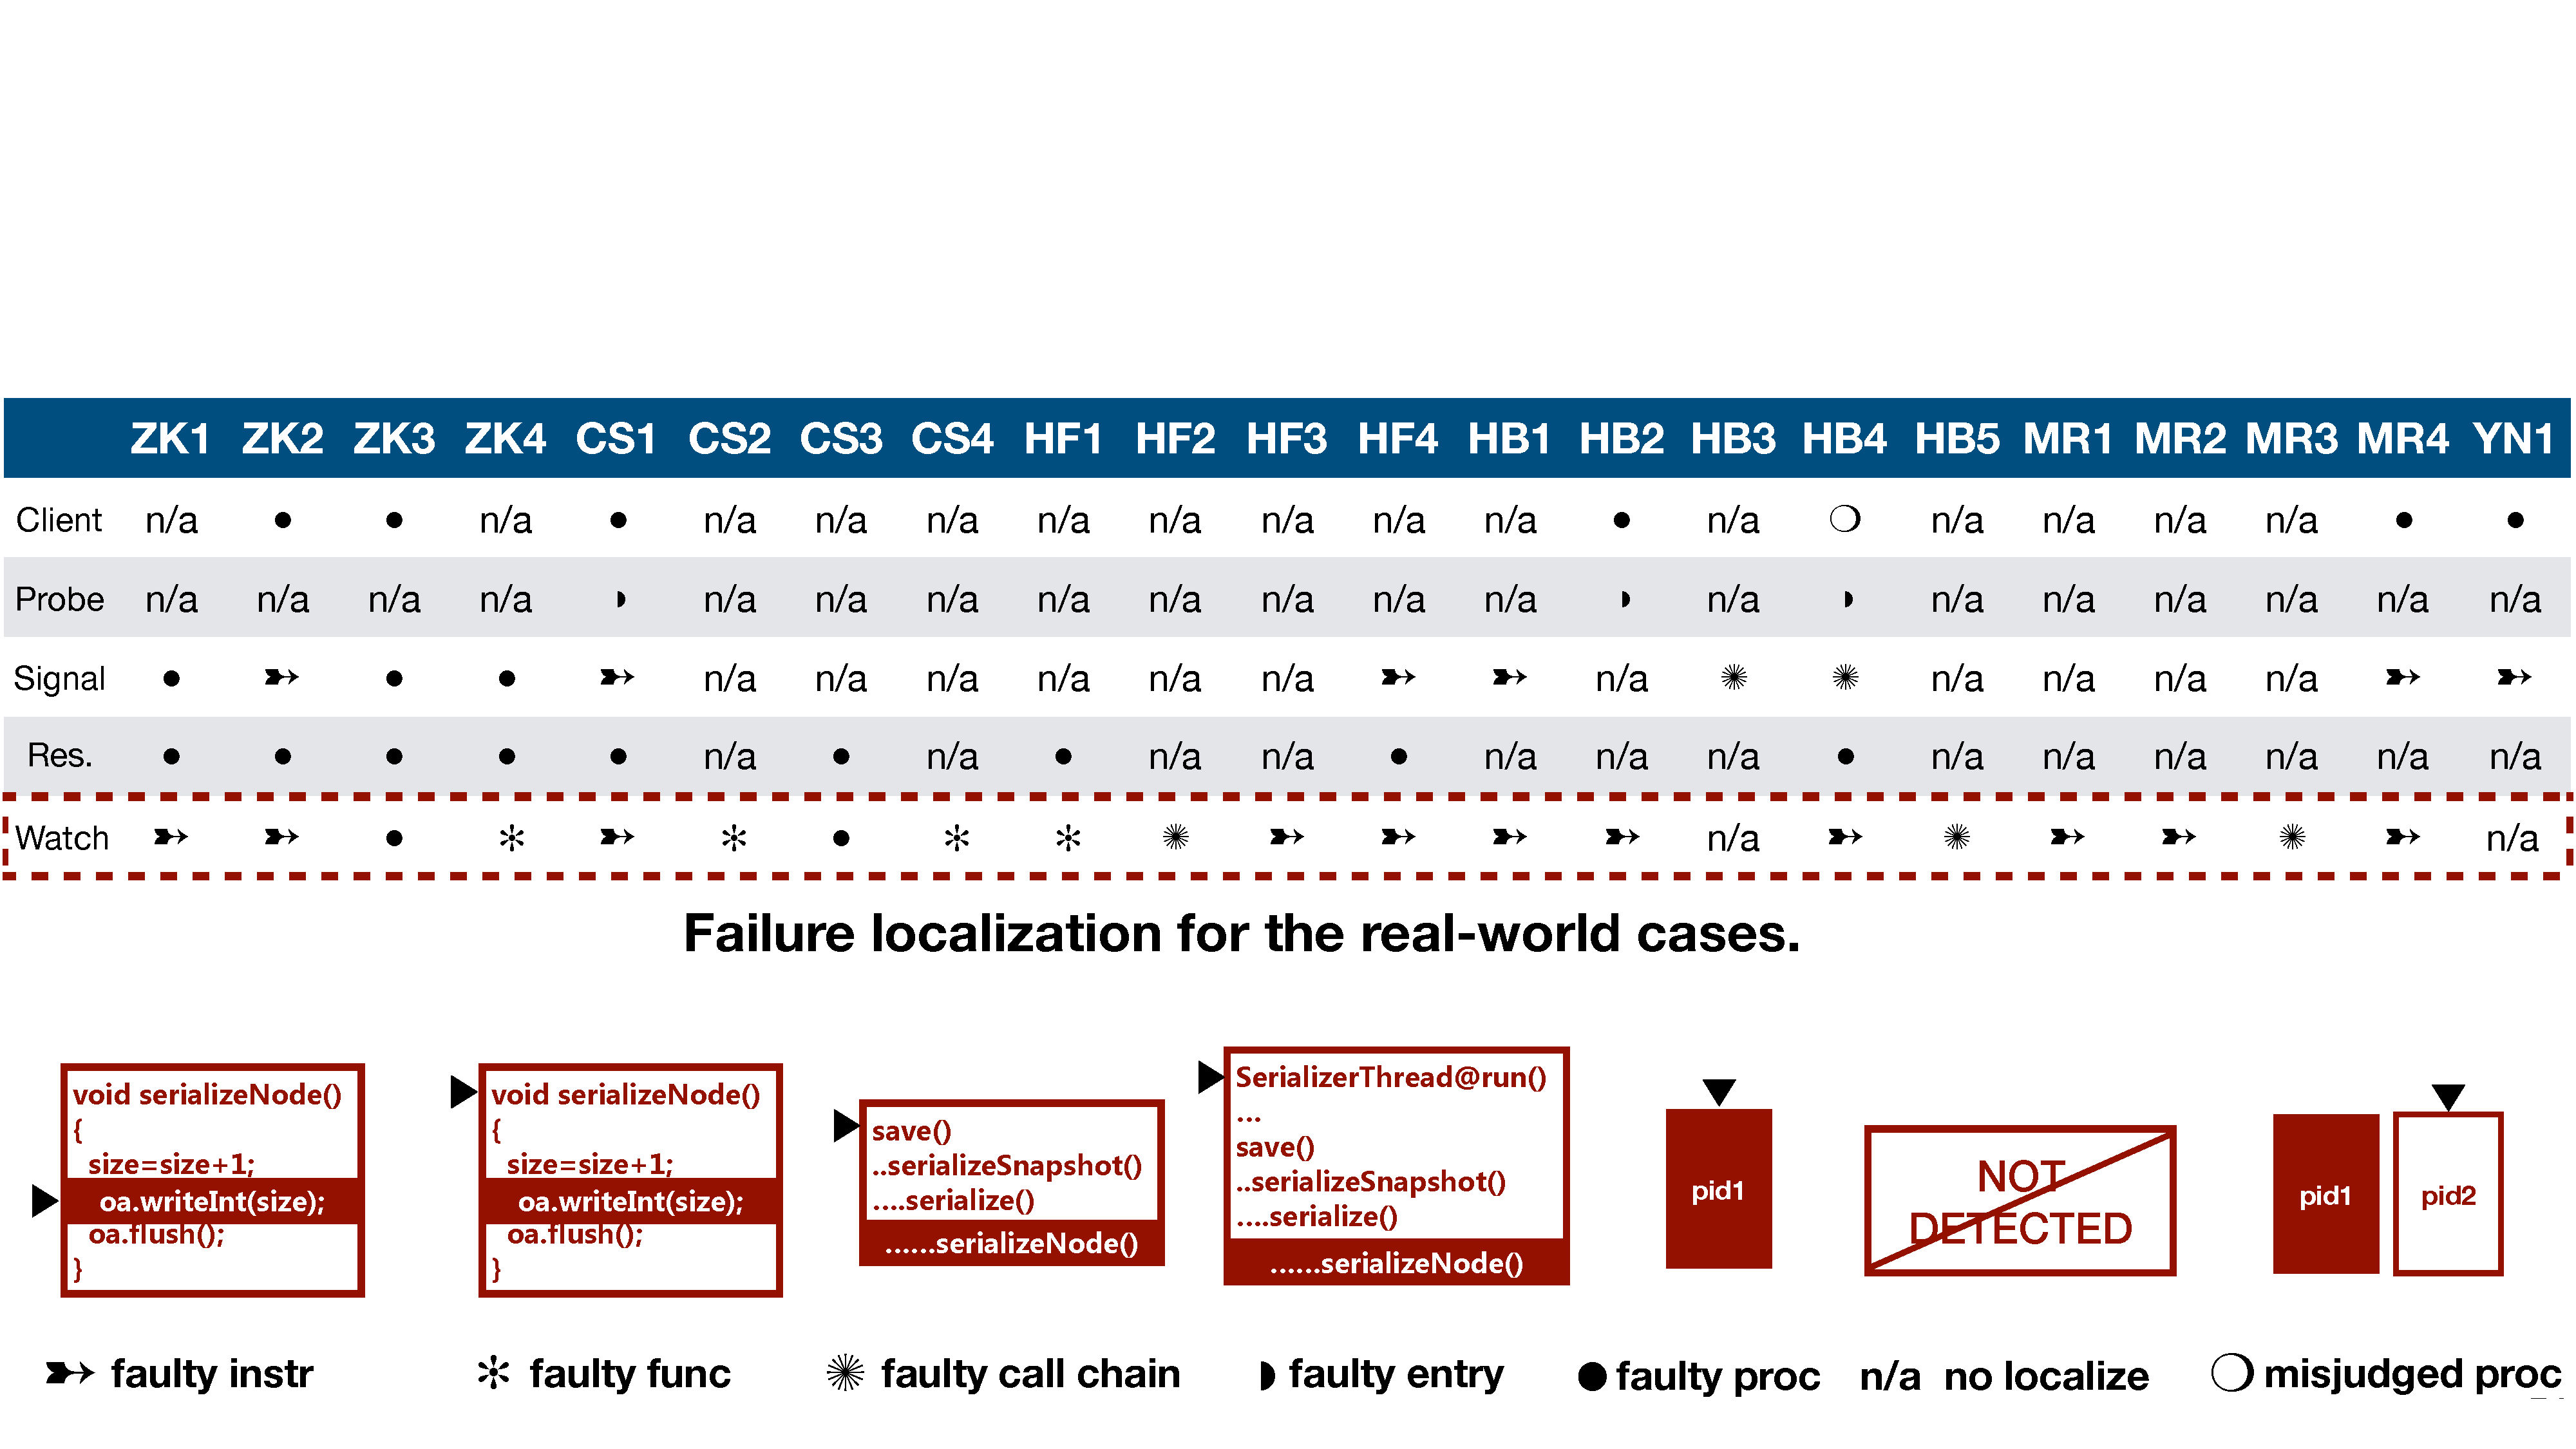
\includegraphics[width=\textwidth]{fig/localization}
\end{frame}

\begin{frame}{False Alarms}
    \framesubtitle{False alarm ratios of all detectors for six systems under various setups}
    \begin{itemize}
        \item validator $\to$ the watchdog false alarm ratios decrease
    \end{itemize}

    \begin{center}
        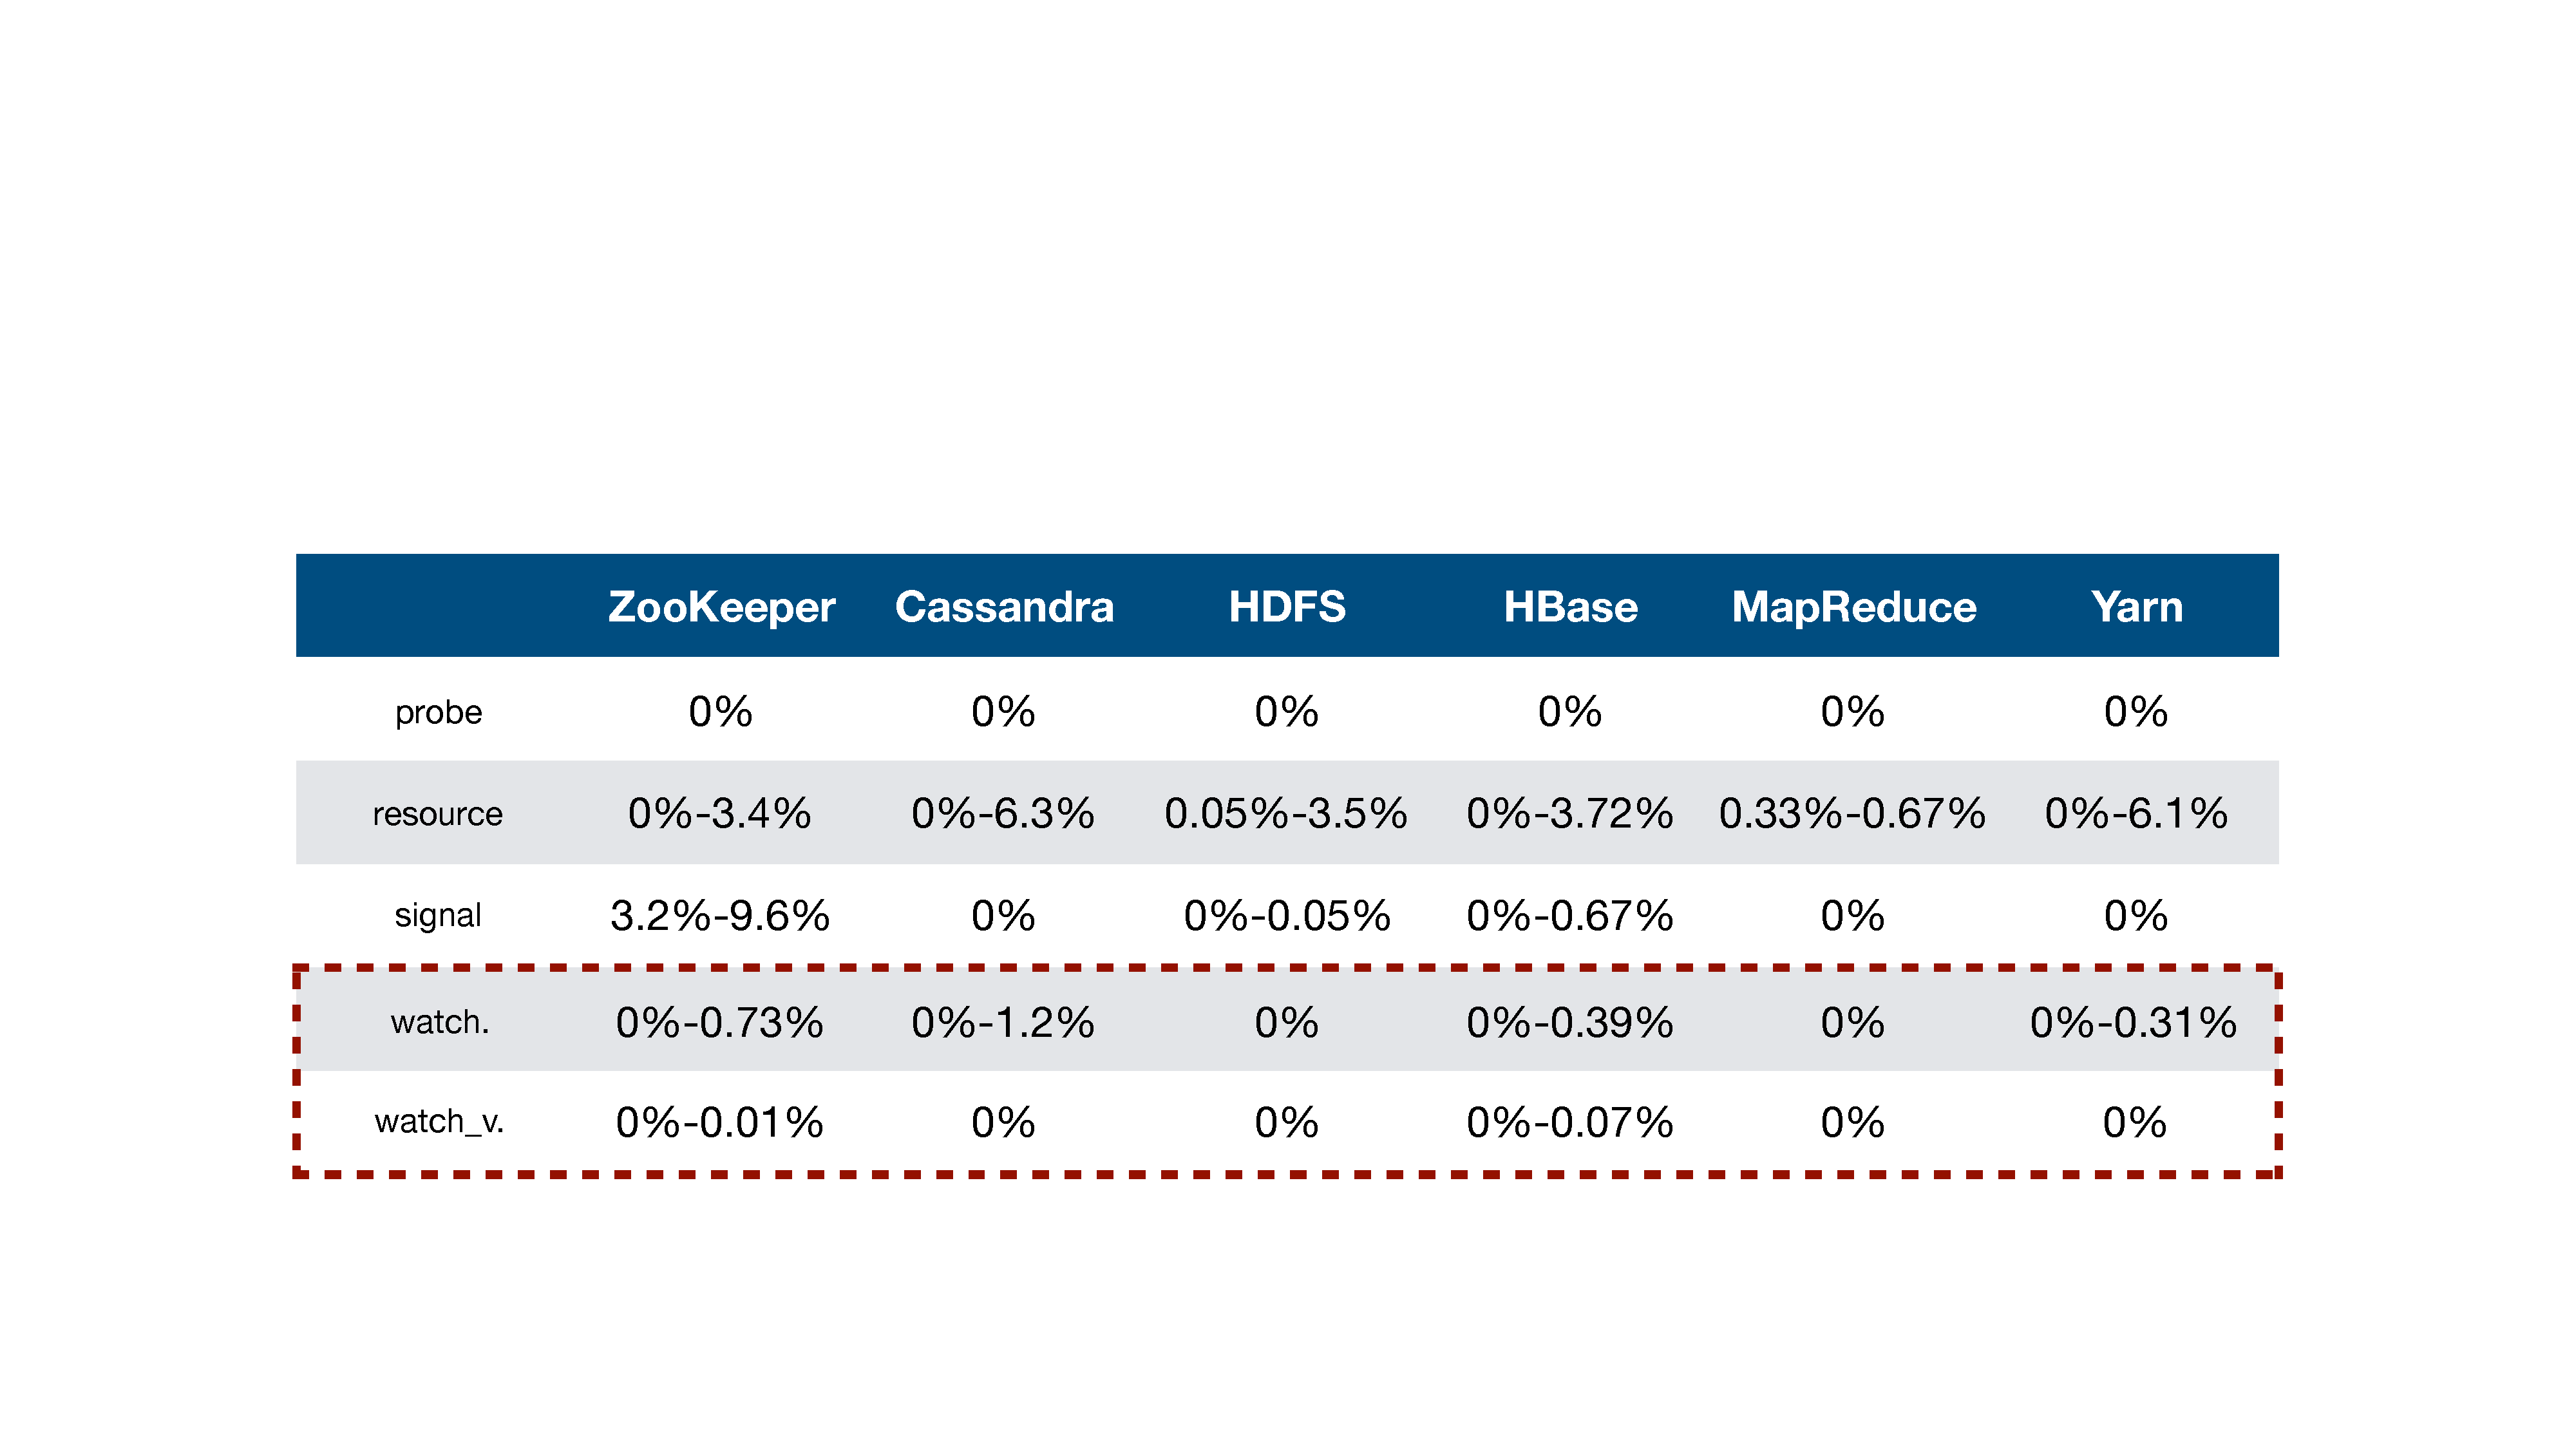
\includegraphics[width=\textwidth]{fig/false-alarm}
    \end{center}
\end{frame}

\begin{frame}{System Overhead}
    \begin{block}{}
        Time to generate watchdogs: 17 min for HBase, $<$ 5 min for the others
    \end{block}
    \begin{columns}
        \begin{column}{.5\textwidth}
            Throughput (op/s) w/ different checkers
            \vspace{1em}
            \begin{center}
                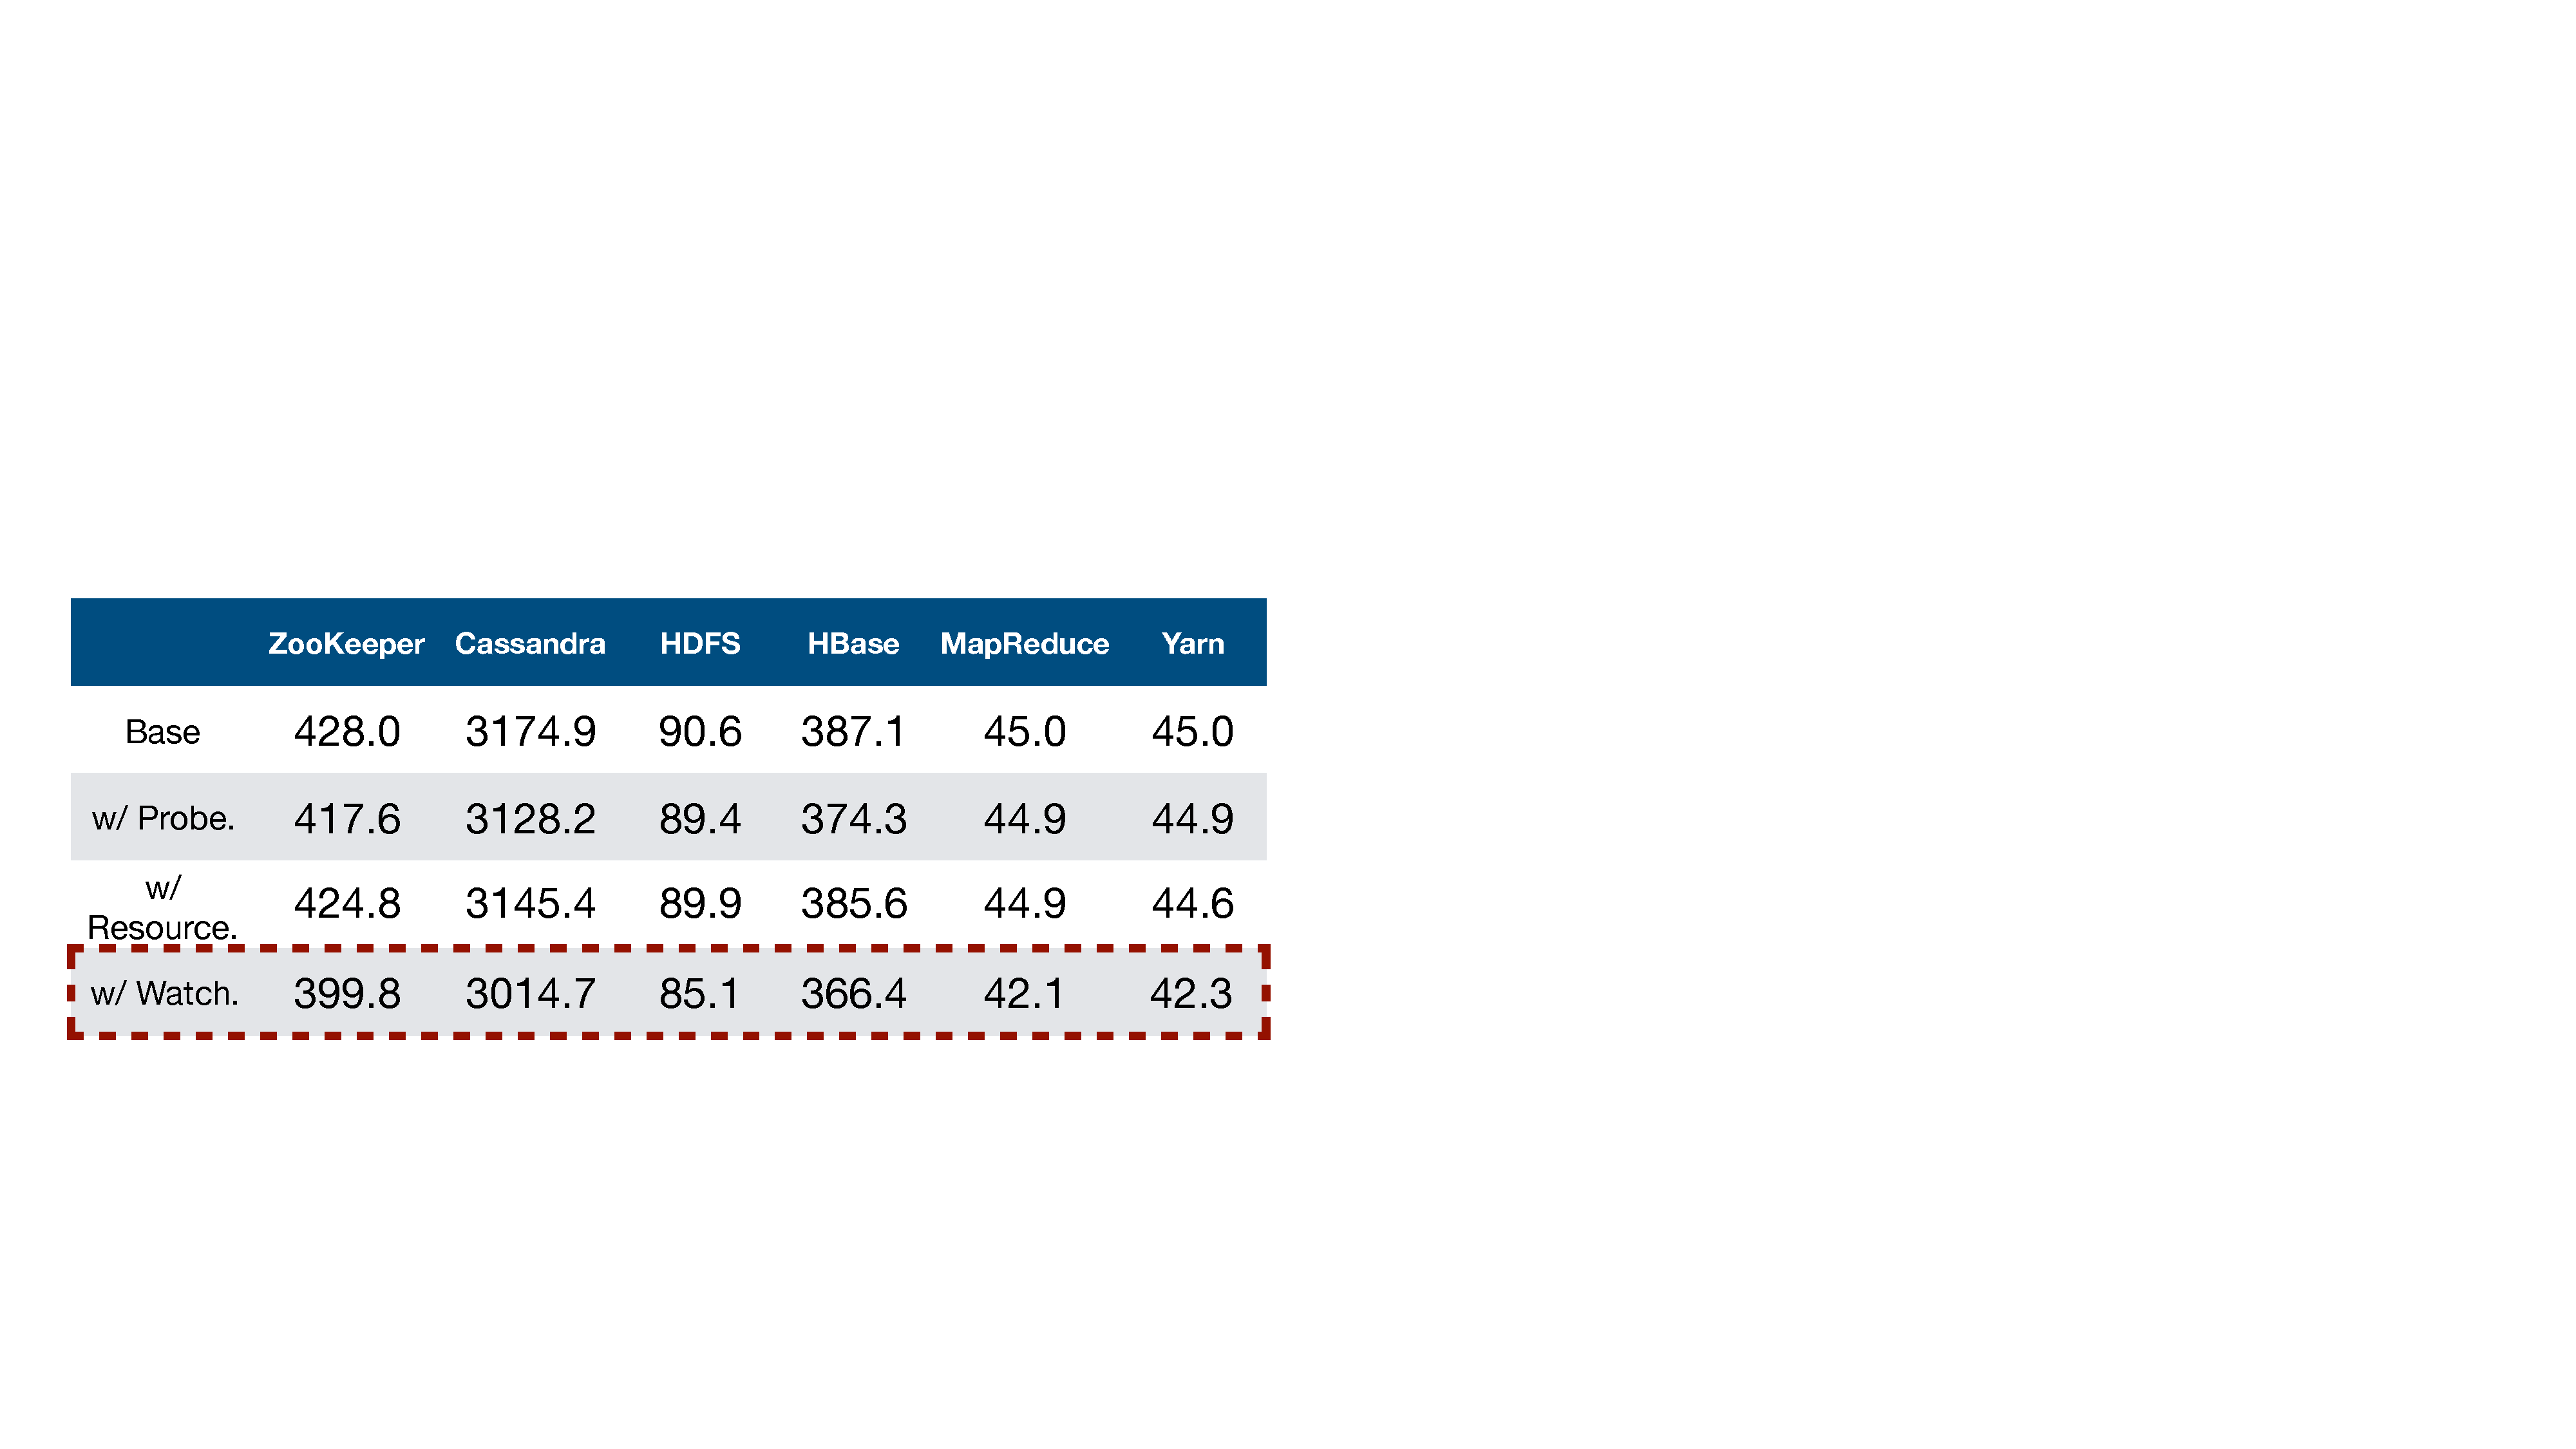
\includegraphics[width=\textwidth]{fig/throughput}

            \end{center}
            \vspace{1em}
            \begin{block}{}
                5.0\%-6.6\% throughput overhead  w/ watchdog
            \end{block}
        \end{column}

        \begin{column}{.55\textwidth}
            Heap memory usage w/ and w/o watchdogs
            \begin{center}
                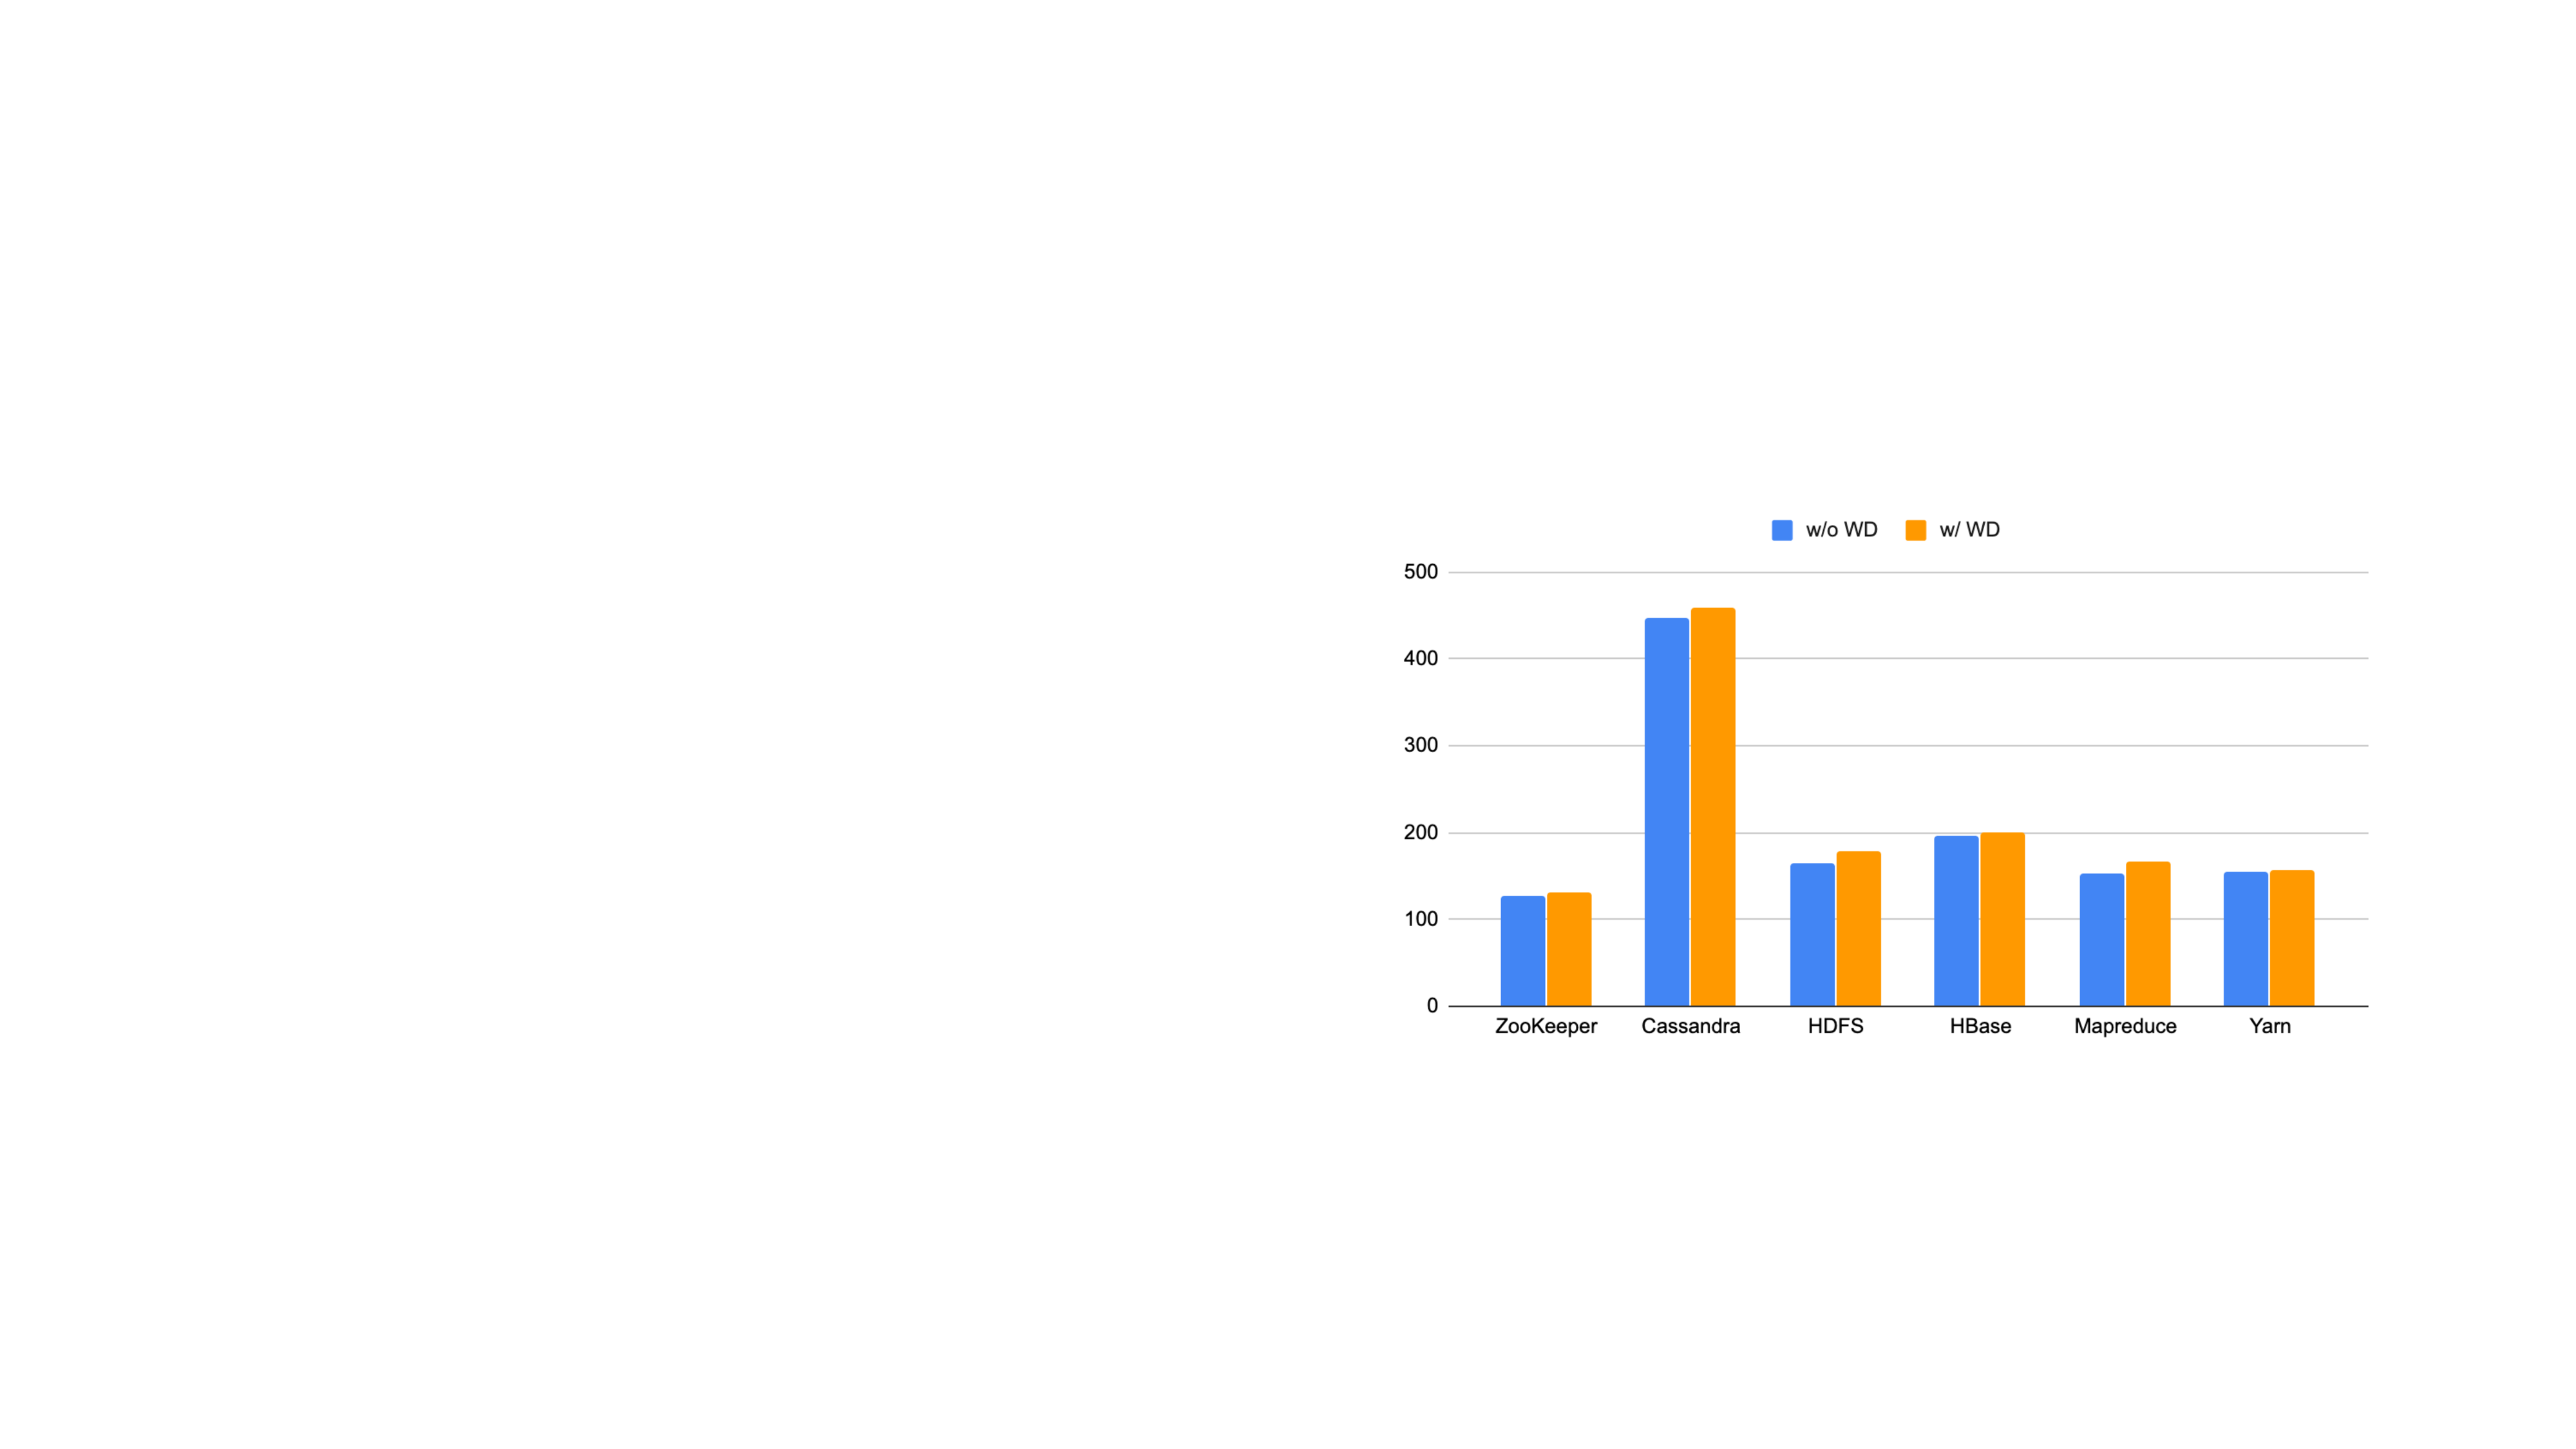
\includegraphics[width=\textwidth]{fig/heap}
            \end{center}
            \begin{block}{}
                4.3\% (avg) memory overhead  w/ watchdog
            \end{block}
        \end{column}
    \end{columns}
\end{frame}

\begin{frame}{By-product: Discovering A New Partial Failure Bug\footnote{Detailed report available at \url{https://issues.apache.org/jira/browse/ZOOKEEPER-3531}}}
    \framesubtitle{Watchdogs report the failure in 4.7 seconds occasionally during experiments}

    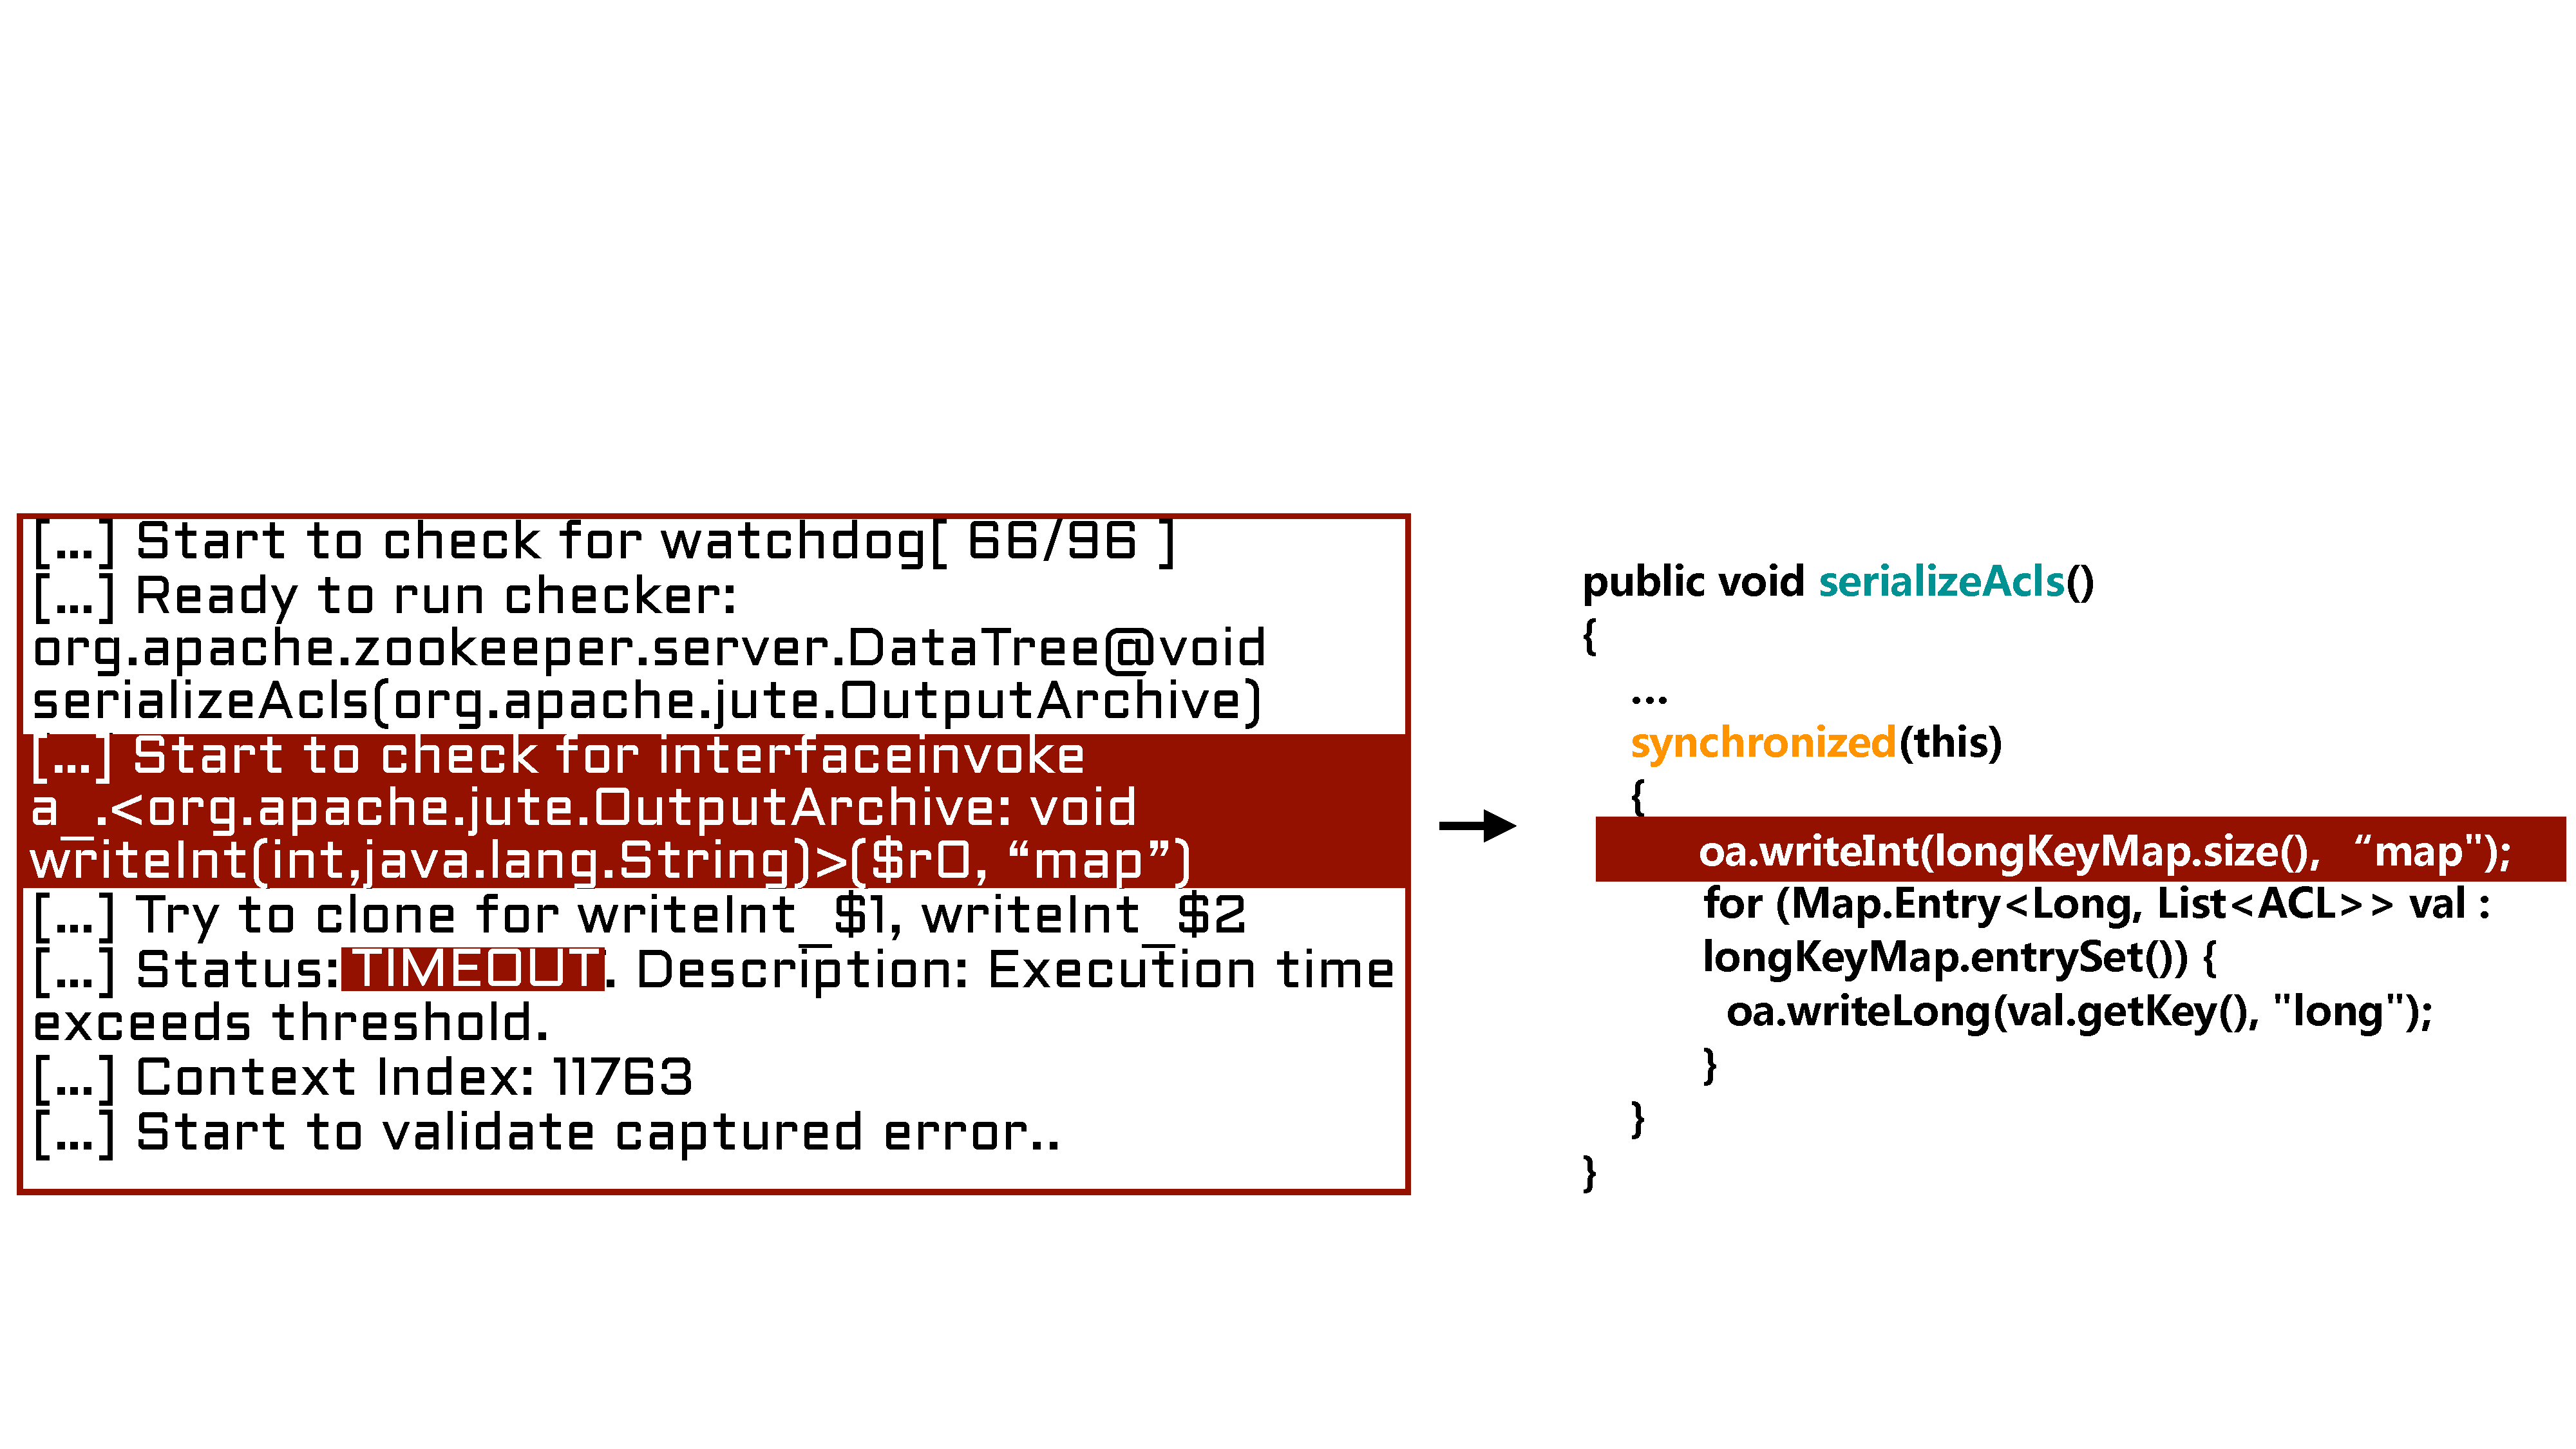
\includegraphics[width=\textwidth]{fig/log}

\end{frame}


\section{Summary}

\begin{frame}{Summary}
    \begin{itemize}
        \item \textbf{Motivation:} Modern software are increasingly complex and often fail
        partially
        \begin{itemize}
            \item these partial failures cannot be detected by process-level failure detectors
        \end{itemize}

        \vspace{1em}

        \item \textbf{Case study:} On 100 partial failure cases
        \begin{itemize}
            \item No main root causes, hard to detect with existing methods
        \end{itemize}

        \vspace{1em}

        \item \textbf{Proposed solution:} \texttt{OmegaGen}: a static analysis tool that automatically generates customized checkers
        \begin{itemize}
            \item successfully generate checkers for six systems and checkers can detect\& localize 18/22 real-world partial failures
            \item watchdog report helps to quickly discover a new bug in the latest zookeeper
        \end{itemize}
    \end{itemize}
\end{frame}

\begin{frame}
    \centering
    \Huge{Thanks}
\end{frame}
\end{document}